% +------- CÓDIGO FONTE TCC -------+
% 	Autor: Arllem Farias, 2017.
% 	E-mail: arllemfarias@ufam.edu.br
%   Revisor: João Victor Lima Lopes
%   E-mail: jvllopess@gmail.com
% +--------------------------------+

% Ítens como: Ficha Catalográfica, Folha de Aprovação Assinada e Lombada, devem ser adicionadas posteriormente
% e descomentar as linhas que as adicionam (Linhas 132,134 e 135).

% Classe do documento --> \documentclass[OPÇÕES]{CLASSE}
\documentclass[
			   a4paper, % Tipo de papel 
			   oneside, % Impressão em apenas um lado da folha
			   12pt     % Tamanho da fonte
			   ]{book}  % Classe do documento

% Pacotes --> \usepackage[OPÇÕES]{PACOTE}
\usepackage[utf8]{inputenc} % Codificação do documento (conversão automática dos acentos) 
\usepackage[brazil]{babel}  % Traduz palavras chaves para o PT-BR (ex.: abstract->resumo)
\usepackage{indentfirst}    % Indenta o primeiro parágrafo de cada seção
\usepackage{setspace}		% Possibilita a alteração do espaçamento entre linhas
\usepackage{graphicx}       % Possibilita a inserção de figuras
\usepackage{subcaption}     % Possibilita a inserção de subfiguras
\usepackage{pdfpages}       % Possibilita a inserção de páginas em pdf
\usepackage{amsmath}        % Inclui funções adicionais no ambiente matemático \eqref{•} \dfrac{•}{•}
\usepackage{amssymb} 		% Símbolos adicionais no documento \mathbb{R}
\usepackage{mathrsfs}       % Símbolos da transformadas de Laplace e Fourier \mathscr{•}
\usepackage{float}			% Possibila posicionar tabelas e figuras em uma posição específica [H]
\usepackage[numbers]{natbib}% Inclui mais possibilidades de citações \citep{•}
\usepackage{fancyhdr}       % Possibilita a alteração de cabeçalho e rodapé
\usepackage{longtable}      % Possiblita a quebra de tableas em duas páginas
\usepackage{multirow}		% Possibilita multiplas linhas em tabelas
\usepackage{array}			% Possibilita o uso do comando \newcolumntype{•}[•]
\usepackage{pdflscape}      % Possibilita a inserção de páginas em modo paisagem
\usepackage{listings}		% Possibilita inserir códigos fontes (C++, Java, ...)
\usepackage{slashbox}       % Adiciona o comando \backslashbox{•}{•} usado em tabelas
\usepackage{arydshln}       % Possibilita inserir linhas pontilhadas em tabelas 
\usepackage[portuguese, ruled]{algorithm2e}

%\usepackage[inline]{showlabels} % Mostra os labels das equações
%\usepackage[notcite,notref]{showkeys} % Mostra todo os labels
%\usepackage{lipsum} % preenchimento automático de textos

% Modifica os itens do sumário
\usepackage[nottoc,
			notlof,
			notlot]{tocbibind}

% Configura as margens das páginas
\usepackage[top    = 3cm,
			bottom = 2cm,
			left   = 3cm,
			right  = 2cm]{geometry}

% Possibilita hiperlinks no texto
\usepackage[pdftex,
			%backref,
			linktocpage = false,
			colorlinks  = true,
			linkcolor   = blue,
			anchorcolor = blue,
			citecolor   = blue,
			urlcolor    = blue]{hyperref}

% Comandos auxiliares --> \nomecomando{COMANDO}{•}
\newcolumntype{C}[1]{>{\centering\let\newline\\\arraybackslash\hspace{0pt}}m{#1}} % Tabelas: {|C{2cm}|C{5cm}|}
\newcolumntype{L}[1]{>{\let\newline\\\arraybackslash\hspace{0pt}}m{#1}} % Tabelas: {|L{2cm}|L{5cm}|}
\newcommand*{\doi}[1]{DOI: \href{http://dx.doi.org/#1}{#1}} % Usado nas referencias

\setcounter{secnumdepth}{3} % Inclui a numeração de \subsubsection{•} no documento
\setcounter{tocdepth}{3}    % Inclui a \subsubsection{•} no sumário
\setstretch{1.5}			% Configura o espaçamento entre linhas \usepackage{setspace}

\pagestyle{fancy} 			% Configura a página para incluir o cabeçalho e rodapé
\lhead{{\footnotesize\leftmark}} % Cabeçalho esquerdo
\chead{}				         % Cabeçalho central
\rhead{\thepage}				 % Cabeçalho direito
\fancyfoot{}					 % Rodapé vazio

% Definição de novas cores
\definecolor{mygreen}{RGB}{0, 115, 0}
\definecolor{mylilas}{RGB}{170,55,240}

\lstset{ % -> \usepackage{listings}
  language=Matlab,
  basicstyle=\ttfamily\small, 
  morekeywords={matlab2tikz},
  keywordstyle=\color{blue}, 
  stringstyle=\color{mylilas}, 
  commentstyle=\color{mygreen}, 
  extendedchars=true,
  showspaces=false,
  showstringspaces=false,
  numbers=left,
  numberstyle=\tiny,
  breaklines=true,
  breakautoindent=true,
  captionpos=b,
  xrightmargin=0pt,
  xleftmargin=15pt,
}


% Novos comandos --> \newcommand{COMANDO}{DEFINIÇÃO}
\newcommand{\instituicao}{
				UNIVERSIDADE FEDERAL DO AMAZONAS\\
				FACULDADE DE TECNOLOGIA\\
				ENGENHARIA DA COMPUTAÇÃO}
\newcommand{\titulo}{
				Identificação e Controle de um Levitador à Ar}
\newcommand{\apresentacao}{
				Monografia apresentada à Coordenação do Curso
				de Engenharia da Computação da Universidade Federal
				do Amazonas, como parte dos requisitos necessários
				à obtenção do título de Engenheiro de Computação.}
\newcommand{\autor}{
				Mateus Martínez de Lucena}
\newcommand{\local}{
				MANAUS-AM\\2018}
\newcommand{\orientador}{
				Iury Valente de Bessa}

%-----------------------------------------------------
\usepackage{ulem}
\newcommand{\commentib}[1]{{\color{red} [IB: #1]}}
\newcommand{\corrigir}[1]{{\color{violet}\uwave{#1}}}
\newcommand{\cortar}[1]{{\color{violet}\sout{#1}}}
\newcommand{\melhorar}[1]{{\color{green}\uwave{#1}}}
%-----------------------------------------------------

\begin{document}

\begin{titlepage}

\begin{center}

\begin{figure}[t]
	\centering
	\includegraphics[scale=0.7]{pasta1_figuras/logo_ufam.eps}
\end{figure}

\textbf {\instituicao}

\vfill
\textbf{\Large \titulo}

\vfill
\textbf{\autor}

\vfill
\textbf{\local}

\end{center}

\end{titlepage}

%\begin{titlepage}
	
\includepdf{parte1_pre-textuais/lombada_tcc.pdf}
		
\end{titlepage}



\thispagestyle{empty}

\begin{center}

\autor

\vfill {\Large \titulo}

\vfill{
\begin{flushright}
	\begin{minipage}{8cm} 
		\apresentacao
	\end{minipage}
\end{flushright}
}

\vfill Orientador: \orientador

\vfill	\local

\end{center}

%\thispagestyle{empty}

\includepdf{parte1_pre-textuais/ficha_catalografica_ufam.pdf}

%\thispagestyle{empty}

\includepdf{parte1_pre-textuais/folha_de_aprovacao_assinada.pdf}

\thispagestyle{empty}

\vspace*{\fill}
\begin{flushright}
	\begin{minipage}{8cm}
		\textit{
			\qquad DEDICATÓRIA AQUI
		}
	\end{minipage}
\end{flushright}

\chapter*{Agradecimentos}
\thispagestyle{empty}

Agradeço primeiramente à Deus por todas as bençãos presentes na minha vida e aos meus pais por me motivar a sempre fazer o melhor que podemos fazer em todas as situações. Agradeço ao meu orientador por me guiar durante as dificuldades do projeto. E agradeço finalmente a todos os professores que participaram na minha formação acadêmica.
\thispagestyle{empty}

\vspace*{\fill}
\begin{flushright}
	\begin{minipage}{8cm}
		\textit{
			“Se você cumprir suas obrigações todo dia você não tem que se preocupar com o futuro.”
			{(Dr. Jordan B. Peterson)}
		}
	\end{minipage}
\end{flushright}



\chapter*{Resumo}
\thispagestyle{empty}

No estudo do controle de sistemas nos deparamos com variados sistemas clássicos 

\vspace{50pt}

\paragraph{Palavras-chave:} PALAVRAS CHAVES AQUI.

\chapter*{Abstract}
\thispagestyle{empty}

ABSTRACT AQUI

\vspace{50pt}

\paragraph{Keywords:} KEYWORDS HERE.



\pagenumbering{roman}

\listoffigures

%\thispagestyle{empty}

\listoftables

%\thispagestyle{empty}

\markboth{\MakeUppercase{Lista de Abreviaturas e Siglas}}{\MakeUppercase{Lista de Abreviaturas e Siglas}}

\chapter*{Lista de Abreviaturas e Siglas}

\begin{longtable}{lL{14cm}L{\textwidth}}

\textbf{PRBS}  & Sinal Binário Pseudo Aleatório -- do inglês Pseudo Random Binary Signal & \\

\textbf{E.D.O.}  & Equação Diferencial Ordinária & \\

\textbf{ARX}  & Auto regressivo com termos exógenos -- do inglês Autoregressive with exogenous terms & \\

\textbf{SISO}  & Entrada única saída única -- do inglês Single Input Single Output & \\

\textbf{BIBO}  & Entrada limitada saída limitada -- do inglês Bounded Input Bounded Output & \\

\textbf{PE Condition}  & Condição de excitação permanente -- do inglês Permanent Excitement Condition & \\

\textbf{PVC}  & Policloreto de polivinila& \\

\textbf{RC}  & Controle remoto -- do inglês Remote Control & \\
\textbf{MPC} & do inglês Model Predictive Control &\\

\textbf{PWM} & Modulação em largura de pulsa -- do inglês Pulse Width Modulation & \\

\end{longtable}

\markboth{\MakeUppercase{Lista de Símbolos}}{\MakeUppercase{Lista de Símbolos}}

\chapter*{Lista de Símbolos}

\begin{spacing}{1.45}

\noindent \textbf{Símbolos Matemáticos}

\begin{longtable}{L{1.5cm}L{14cm}L{\textwidth}}

$\mathbb{R}$ & conjunto dos números reais & \\
$\varphi$ & matriz de regressores dos mínimos quadrados &\\
${\{ \cdot \}}^\dagger$ & pseudo inversa &\\





\end{longtable}

\end{spacing}

\tableofcontents

%\thispagestyle{empty}


\pagenumbering{arabic}

\chapter{Introdução} %Contextualização, motivação e justificativa.

\section{Levitação a ar}

O túnel de vento é uma instalação utilizada para estudar o desempenho aerodinâmico de objetos. Ele é feito de um duto de tamanho adequado para o objeto testado pelo qual o ar flui ao ser empurrado por uma turbina. Os testes feitos variam de velocidade de acordo com o que se deseja estudar, os ventos podem ser subsônicos, supersônicos ou hipersônicos.


Para que os testes sobre objetos tenham resultados precisos e replicáveis a velocidade dos ventos sobre eles deve ser controlável e atinja o objeto sem turbulência, apesar de haver testes onde isso é proposital. O túnel é construído com estabilizadores que possibilitam reduzir a turbulência do vento.


Os testes geralmente são feitos em modelos em escala de aviões, carros, naves espaciais, e para  estudo da aerodinâmica de objetos na física. Os túneis podem ser verticais ou horizontais, apesar de os túneis horizontais existirem em maior quantidade. Um teste comum é feito em modelos de aviões onde se medem as propriedades das asas como envergadura ao ser submetida a velocidades específicas do vento, força de elevação para diferentes velocidades e em geral sua aerodinâmica. Em Dayton, Ohio\cite{vertical1946}, foi construído um túnel de vento vertical que possibilita que sejam feitos testes específicos para aeronaves. Um objeto é posto em queda livre virtual devido a velocidade do vento impulsionado por uma turbina e se observa o seu movimento na situação. Este teste foi essencial para a prototipagem de aviões militares e comerciais desde os anos 50.


Hoje os testes ainda são responsáveis por economizar milhões de reais na fase de prototipagem em testes aerodinâmicos, no desenvolvimento de trens de alta velocidade\cite{KWON2001}. Em objetos que se movem em alta velocidade o vento se torna um fator preocupante, uma rajada de vento pode ser o fator determinante em um descarrilhamento de um trem, os testes possibilitam que os cientistas analisem  comportamento de suas criações em situações previsíveis e os ajuda a antecipar possíveis problemas.

No entanto, existe um problema no teste aerodinâmico utilizando túneis de vento. Para os testes de queda livre como o de aeronaves, o controle de altitude do objeto é complexo. É possível obter o número de Reynolds, uma variável sem dimensão que possibilita predizer o padrão de fluxo de fluídos, e é possível medir a velocidade do vento atuando em cima do objeto, porém, a real dificuldade se encontra no fato de que quando o a força do vento atua em cima de um objeto ele se comporta de maneria quase imprevisível. Uma bola gira em várias direções, por exemplo.


Tendo em vista que o controle de altura de um objeto tendo como único atuador o vento, e que um modelo de atuação da força do vento sobre um objeto é complexo e de baixa fidelidade, e que precisamos de um modelo que possibilite um controle de altitude preciso e robusto, temos como opção a modelagem caixa-preta, conhecida como identificação de sistemas.


\section{Objetivos}

\subsection{Objetivos Gerais}
O objetivo principal deste trabalho é fazer uma comparação qualitativa entre dois tipos de identificação de sistemas, uma por mínimos quadrados que resulta em um modelo ARX do sistema, e uma por subespaços que resulta em um modelo em espaço de estados, e controle do sistema.

\subsection{Objetivos Específicos}
\begin{itemize}
	\item Construir uma plataforma de experimento no formato de túnel de vento.
	\item Medir a velocidade do vento em alturas variadas dentro do túnel de vento.
	\item Criar um simulador para o túnel de vento.
	\item Executar testes para identificação usando como sinal de controle um sinal binário pseudo aleatório (PRBS).
	\item Identificar o sistema por mínimos quadrados.
	\item Identificar o sistema por subespaços.
	\item Validar os modelos obtidos.
	\item Obter um controlador para os dois modelos usando alocação de polos.
\end{itemize}

\section{Organização do trabalho}
Este trabalho se encontra organizado em sete capítulos com várias subseções. O primeiro é a introdução onde o trabalho é contextualizado e apresentado, os objetivos são explicitados e a organização do trabalho é explicada. O segundo capítulo é a revisão bibliográfica com as seções fundamentação teórica onde conceitos fundamentais ao entendimento do trabalho são explicados, e trabalhos relacionados onde o trabalho de outros autores é relacionado a este. O terceiro capítulo fala sobre a modelagem e simulação do túnel de vento. O quarto capítulo trata da identificação do túnel usando mínimos quadrados e subespaços. O quinto é projeto de controladores. O sexto capítulo trata da avaliação experimental do sistema de controle. O sétimo e último capítulo é a conclusão do trabalho onde as considerações finais e trabalhos futuros serão discutidos.

% Fim Capítulo
\chapter{Revisão Bibliográfica} \label{cap2}
Nesta seção serão apresentadas duas subseções importantes para o entendimento deste trabalho, a revisão bibliográfica que trata de conceitos fundamentais ao entendimento do trabalho, e trabalhos relacionados que trata de outros trabalhos que são pertinentes à este.
	
\section{Fundamentação Teórica}
Nesta subseção tratamos de conceitos essenciais para o entendimento deste trabalho. Falaremos sobre alguns modelos matemáticos, critérios de estabilidade de sistemas discretos, e métodos de identificação de sistemas e estimação de parâmetros, em especial identificação por mínimos quadrados e por subespaços.


\subsection{Modelos de Sistemas Dinâmicos}\label{capA}
O modelo matemático de um sistema dinâmico é uma forma de descrever uma parte do fenômeno físico que queremos controlar. Nesta seção serão apresentados alguns dos vários modelos matemáticos relacionados ao projeto.
\subsubsection{Equação Diferencial Ordinária}
Um sistema dinâmico pode ser modelado usando somente a descrição matemática do fenômeno desejado. Usamos como exemplo a modelagem do amortecimento em uma roda de um carro, visto na figura \ref{fig:modeloamortecimento}.

\begin{figure}
	\centering
	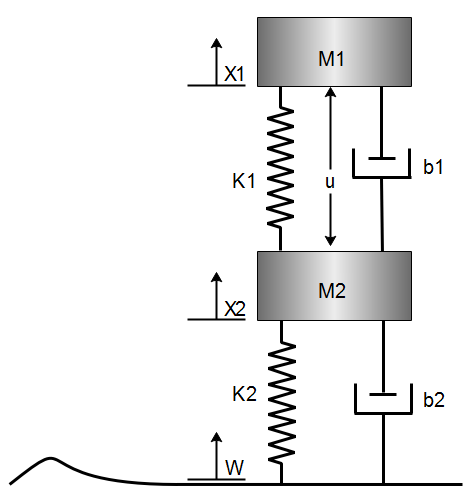
\includegraphics[width=0.5\linewidth]{modelo_amortecimento}
	\caption{Esquema do amortecedor da roda de um carro}
	\label{fig:modeloamortecimento}
\end{figure}

Onde $X_1$ e $X_2$ são a altura das massas $M_1$ e $M_2$, massa do carro e massa da roda, respectivamente. $K_1$ é o efeito elástico do amortecedor e $K_2$ é o efeito elástico da roda. $b_1$ é o efeito amortecedor da suspensão e $b_2$ é o efeito amortecedor da roda.
Esse sistema pode ser modelo em uma E.D.O. (Equação Diferencial Ordinária) usando as leis de Newton, visto nas equações \eqref{eq:edo1} e \eqref{eq:edo2}.

\begin{equation} \label{eq:edo1}
M_1 \ddot{X}_1=-b_1(\dot{X}_1-\dot{X}_2) -K_1(X_1-X_2)+U
\end{equation}
\begin{equation} \label{eq:edo2}
M_2 \ddot{X}_2=b_1 (\dot{X}_1 -\dot{X}_2) +K_1(X_1-X_2) +b_2(\dot{W} -\dot{X}_2)+K_1(W-X_2) -U
\end{equation}

\subsubsection{Funções de Transferência}
A função de transferência é uma equação que descreve o comportamento dinâmico de um sistema relacionando uma entrada com uma saída. Ela é a transformada de Laplace da resposta ao impulso do sistema.

Usando o mesmo sistema da figura \ref{fig:modeloamortecimento} e aproveitando as equações \eqref{eq:edo1} e \eqref{eq:edo2} podemos encontrar as equações de transferência referentes às saídas $X_1$ e $X_2$.

Aplicamos a transformada de Laplace nas equações $X_1$ e $X_2$ para obter:
\begin{equation} \label{eq:e2121}
(M_1s^2+b_1s+K_1) X_1(s) -(b_1s+K_1) X_2(s)=U(s)
\end{equation}
\begin{equation} \label{eq:e2122}
-(b_1s+ K_1) X_1(s) +(M_2s^2 + (b_1 + b_2)s +(K_1 + K_2))X_2(s)=(b_2s +K_2) W(s)-U(s)
\end{equation}
Fazendo as devidas manipulações matemáticas chegamos à função de transferência.
\begin{equation}\label{eq:e2123}
\begin{array}{c}
G_1(s)=\dfrac{X_1(s)-X_2(s)}{W(s)}= \dfrac{(M_1+M_2)s^2+b_2s+K_2} {\Delta}
\\
G_2(s)=\dfrac{X_1(s)-X_2(s)}{W(s)}= \dfrac{-M_1b_2s^3-M_1K_2s^2}{\Delta}
\\
\Delta=(M_1s^2+b_1s+K_1)\cdot (M_2s^2+ (b_1+b_2)s+(K_1+K_2))-(b_1s+K_1)\cdot (b_1s+K_1)
\end{array}
\end{equation}

Com as equações descritas em \eqref{eq:e2123} temos uma equação representando a transferência da entrada para a saída.
\subsubsection{Espaço de Estados}
A representação em espaço de estados é uma forma mais conveniente para representar sistemas no domínio do tempo quando existe mais de uma entrada ou saída do que a função de transferência. Um modelo linear é representado tipicamente no seguinte formato:
\begin{equation}\label{eq:ss}
\begin{array}{c}
\dot{x}=Ax+Bu\\
y=Cx+Du
\end{array}
\end{equation}
Onde $x \in \Re^n$ é o vetor de estado n-dimensional. $\dot{x}=dx/dt$, $u(t) \in \Re^p$ é o vetor de entradas formado por r funções temporais, $y(t) \in \Re^q$ é o vetor m-dimensional de saídas e $A \in \Re^{n\times n}$, $B \in \Re^{n \times p}$, $C \in \Re^{q \times n}$ e $D \in \Re ^{q \times p}$ são as matrizes do sistema constantes.


Podemos gerar uma representação de espaço de estados a partir da E.D.O. do sistema. Vamos utilizar novamente o sistema da figura \ref{fig:modeloamortecimento}. Definimos primeiramente os estados do vetor x, $x_1=X_1$, $x_2=\dot{X}_1$, $x_3=Y_1$ e $x_4=\dot{Y}_1$. Onde $Y_1=X_1-X_2$, geramos então as matrizes do espaço de estados usando as equações \eqref{eq:edo1} e \eqref{eq:edo2}:
\begin{equation}
\begin{bmatrix}
\dot{X}_1\\
\ddot{X}_1\\
\dot{Y}_1\\
\ddot{Y}_1
\end{bmatrix}
=
\begin{bmatrix}
0 & 1 & 0 & 0\\
\dfrac{-b_1b_2}{M_1M_2} & 0 &\left[ \dfrac {b_1} {M_1} \left( \dfrac {b_1} {M_1} + \dfrac{b_1}{M_2} +\dfrac{b_2}{M_2} \right)- \dfrac{K_1}{M_1}\right] & \dfrac{-b_1}{M_1}\\
\dfrac{b_2}{M_2} & 0 & -\left( \dfrac{b_1}{M_1}+ \dfrac{b_1}{M_2}+ \dfrac{b_2}{M_2} \right) & 1\\
\dfrac{K_2}{M_2} & 0 & -\left( \dfrac{K_1}{M_1} +\dfrac{K_1}{M_2}+ \dfrac{K_2}{M_2} \right) & 0
\end{bmatrix}
\begin{bmatrix}
X_1\\\dot{X}_1 \\Y_1 \\ \dot{Y}_1
\end{bmatrix}
+
\begin{bmatrix}
0 & 0 \\
\dfrac{1}{M_1} & \dfrac{b_1b_2}{M_1M_2}\\
0 & \dfrac{-b_2}{M_2} \\
\left( \dfrac{1}{M_1}+ \dfrac{1}{M_2} \right) & \dfrac{-K_2}{M_2}
\end{bmatrix}
\begin{bmatrix}
U\\W
\end{bmatrix}
\end{equation}
\begin{equation}
Y=
\begin{bmatrix}
0 & 0 & 1 & 0
\end{bmatrix}
\begin{bmatrix}
X_1\\\dot{X}_1\\Y_1\\\dot{Y}_1
\end{bmatrix}
+
\begin{bmatrix}
0 & 0
\end{bmatrix}
\begin{bmatrix}
U \\W
\end{bmatrix}
\end{equation}

\subsubsection{Modelo ARX}
O modelo ARX SISO linear tem o seguinte formato:
\begin{equation}\label{eq:ARXModel}
	y(t)+a_iy(t-1)+a_2y(t-2)+\dots+a_{na}y(t-na)=
	b_1u(t)+b_2u(t-1)+\dots+b_{nb}u(t-nb+1)+e(t)
\end{equation}

Onde y é a entrada, u é a saída e $e$ é o ruído. Isso implica que a saída $y(t)$ é uma predição a partir de uma média ponderada de entradas e saídas passadas. Os parâmetros $a_{na}$ e $b_{nb}$ podem ser estimados utilizando mínimos quadrados numa coleção de dados entrada-saída.

\subsection{Critérios de Estabilidade de sistemas discretos}

O conceito de estabilidade é extremamente importante para a análise de sistemas dinâmicos. Primeiramente definimos  estabilidade de acordo com mudanças nas condições iniciais. Consideremos a equação \eqref{eq:e22}.

\begin{equation} \label{eq:e22}
x(k+1)=f(x(k),k)
\end{equation}
Sejam $x_0(k)$ e $x(k)$ suas soluções quando as condições inicias são $x_0(k_0)$ e $x(k_0)$. Definimos:


$\bullet$ Estabilidade: A solução $x_0(k)$ é estável se para um dado $\epsilon>0$ existe um $\delta(\epsilon,k_0)$ tal que para todas as soluções com $||x(k_0)-x_0(k_0)||<\delta$ são tais que $||x(k)-x_0(k)||<\delta$ para todos os $k \geqslant k_0$.


$\bullet$ Estabilidade Assintótica: A solução $x_0(k)$ é assintoticamente estável se é estável e um $\delta$ pode ser escolhido tal que  $||x(k_0)-x_0(k_0)||<\delta$ que implica que $||x(k)-x_0(k)||\to\delta$ quando $k \to \infty$.


Existem outros tipos de estabilidade que são de interesse:


$\bullet$Estabilidade BIBO (Bounded-Input Bounded-Output): Um sistema linear invariante no tempo é definido BIBO estável se dado um sinal de entrada limitado ele produz uma saída limitada para cada valor inicial.


Dado que a estabilidade de um sistema é importante para o seu estudo, os métodos para determinar a sua estabilidade são de grande interesse. Os seguintes são alguns dos métodos utilizados para determinar a estabilidade de um sistema:
\begin{itemize}
	\item Cálculo dos autovalores da matriz A da representação de espaços de estado.
	\item Métodos baseados nas propriedades dos polinômios característicos.
	\item O método do lugar das raízes
	\item O método de Lyapunov
\end{itemize}

O cálculo dos autovalores de uma matriz de ordem maior que 2 à mão não é conveniente e em alguns casos é mais fácil calcular a equação característica da forma:
\begin{equation}
A(z)=a_0z^n+a_1z^{n-1}\dots+a_n=0
\end{equation}

E investigar suas raízes utilizando o método do lugar das raízes onde o critério de estabilidade muda para sistemas discretos determinando que para o sistema ser estável todas as raízes devem estar dentro do círculo unitário.

Outro método para determinar a estabilidade de um sistema é o critério de Jury, versão discreta do critério de Routh-Hourwitz. A tabela de Jury é formada da seguinte forma:
\begin{equation}
H(z)=\dfrac{b(z)}{a(z)}=\dfrac{b(z)}{a_0 z^n+a_1 z^{n-1}+\dots+a_n}
\end{equation}
\begin{equation}
\left|
\begin{matrix}
a_0 & a_1& \dots & a_n\\
a_n & a_{n-1}& \dots & a_0\\
b_0 & b_1 & \dots \\
b_{n-1} & b_{n-2} & \dots \\
c_0 & c_1 & \dots \\
\vdots & \vdots
\end{matrix}
\right.
\end{equation}
onde
\begin{equation}
\begin{matrix}
b_0=a_0- \dfrac{a_n}{a_0}a_n\\
b_1=a_1- \dfrac{a_n}{a_0}a_{n-1}\\
\vdots \\
b_k=a_k- \dfrac{a_n}{a_0}a_{n-k}\\
\vdots \\
c_k=b_k- \dfrac{b_{n-1}}{b_0}b_{n-1-k}\\
\end{matrix}
\end{equation}

Com a tabela formada aplicamos o critério de Jury que diz: se $a_0>0$, então todas as raízes estarão dentro do círculo unitário se e somente se todos os termos da primeira coluna das linhas impares forem positivos. Se nenhum elemento da primeira coluna das linhas impares for nulo, o número  de raízes fora do círculo unitário é igual ao número de elementos negativos.

O segundo método de Lyapunov é outra ferramenta útil para determinar a estabilidade de sistemas dinâmicos não lineares. A ideia é introduzir uma função de energia generalizada chamada função de Lyapunov que é zero no ponto de equilíbrio e positiva em outras posições. O equilíbrio será estável se pudermos mostrar que a função de Lyapunov diminui ao longo das trajetórias do sistema.


O primeiro passo é encontrar a função de Lyapunov definida como segue:


V(x) é uma função de Lyapunov do sistema
\begin{equation}\label{eq:lyap}
x(k+1)=f(x(k)) \qquad f(0)=0
\end{equation}

se:
\begin{enumerate}
	\item V(x) é contínuo em x e V(0)=0
	\item V(x) é definida positiva
	\item $\Delta V(x)=V(f(x))-V(x)$ é definida negativa
\end{enumerate}

Definimos:


$\bullet$Teorema de estabilidade de Lyapunov: A solução $x(k)=0$ é assintoticamente estável se existir uma função de Lyapunov para o sistema da equação \eqref{eq:lyap}. Se:
\begin{equation}
0<\varphi(||x||)<V(x)
\end{equation}
onde $\varphi(||x||)\to \infty$ quando $||x|| \to \infty$, então a solução é assintoticamente estável para todas as condições iniciais.


A grande dificuldade do teorema de Lyapunov é encontrar uma função de Lyapunov adequada. No entanto, para sistemas lineares como o da equação \eqref{eq:sis}, é fácil determinar uma função de Lyapunov quadrática.

\begin{equation} \label{eq:sis}
x_0(k+1)=\Phi x_0(k) \qquad x_0(0)=a_0
\end{equation}

Tomemos $V(x)=x^TP_x$ como candidato para a função de Lyapunov. O incremento de V é dado por:
\begin{equation}
\begin{array}{c}
\Delta V(x)=V(\Phi x)-V(x)=x^T\Phi ^T P \Phi x-x^TPx\\
=x^T(\Phi ^T P \Phi -P)x=-x^TQx
\end{array}
\end{equation}
Para que V seja uma função de Lyapunov é necessário e suficiente que exista uma matriz definida positiva P que satisfaça a equação \eqref{eq:lyapunov}.
\begin{equation}\label{eq:lyapunov}
\Phi ^T P \Phi - P= -Q
\end{equation}






\subsection{Identificação de Sistemas e Estimação de Parâmetros}
A maior parte das técnicas de controle aplicadas na indústria dependem do conhecimento de um modelo matemático do sistema a ser controlado. Apresentamos alguns dos modelos na seção \ref{capA} e nesta seção apresentaremos alguns dos métodos para obtermos os modelos matemáticos utilizados neste trabalho.


\subsubsection{Visão Geral}
A identificação de sistemas e estimação de parâmetros trata de métodos e práticas que permitem construir modelos dinâmicos de um sistema real a partir de experimentos . Muitas vezes um sistema construído que precisa ser controlado não pode ser modelado devido à limitações matemáticas ou imprecisão na interação dos componentes. Nestes casos utilizamos um método de identificação de sistemas para obter um modelo matemático. A identificação de sistemas se baseia em testar a resposta do sistema à certas entradas e a partir das respostas aproximar o modelo matemático de forma satisfatória.


\subsubsection{Identificação por Mínimos Quadrados}
O método de mínimos quadrados é um dos mais conhecidos e utilizados em várias áreas da ciência e tecnologia. A partir de uma coleção de dados experimentais é possível encontrar um modelo matemático ARX.


Para um sistema SISO em que não conhecemos o seu modelo matemático podemos descrever o seu comportamento durante o teste como um conjunto de funções entrada-saída como na equação \eqref{eq:ARXModel}, pois à partir do conhecimento que temos da modelagem física do sistema podemos deduzir aproximadamente de quantos valores passados de y e de u o nosso sistema estudado depende.


Com os vetores entrada e saída em mão montamos uma matriz de regressores y e u no seguinte formato:

\begin{equation}\label{eq:regressores}
\psi=
\begin{bmatrix}
y(n) & y(n-1) & \dots & y(n-i) & u(n) & u(n-1) & \dots & u(n-j)\\
y(n+1) & y(n) & \dots & y(n-i+1) & u(n+1) & u(n) & \dots & u(n-j+1)\\
\vdots & \vdots & \vdots & \vdots & \vdots & \vdots & \vdots  & \vdots\\
y(n+k) & y(n+k-1) & \dots & y(n+k-i) & u(n+k) & u(n+k-1) & \dots & u(n+k-j)\\
\end{bmatrix}
\end{equation}

Onde $y(n-i)$ é o primeiro valor do vetor de saídas y e $u(n-i)$ é o primeiro valor do vetor de entradas u, i é a quantidade de regressores y que influenciam na saída y e j é a quantidade de regressores u que influenciam na saída y, $n+k$ é o número de valores do vetor de entrada.



Podemos então relacionar o vetor de saídas com a matriz de regressores A da seguinte forma:

\begin{equation}
\begin{array}{c}
\begin{bmatrix}
y_1 \\ y_2 \\ y_3\\ \vdots \\ y_n
\end{bmatrix}
=
\psi
\begin{bmatrix}
\theta_1 \\ \theta_2 \\ \vdots \\ \theta_n
\end{bmatrix}
\\
\hat{y}=\psi \hat{\theta}
\end{array}
\end{equation}
Onde $\hat{y}$ é um vetor que depende da matriz de regressores A e do vetor $\hat{\theta}$. Conhecemos $\hat{y}$ e A, queremos determinar $\hat{\theta}$. Desde que X seja não singular é possível determinar o vetor de parâmetros invertendo a matriz:
\begin{equation}\label{eq:MQ}
\theta=\psi^{-1}y
\end{equation}

A matriz $\psi$, no entanto, não é invertível e para realizarmos $\psi^{-1}$ utilizamos a pseudo inversa, que será utilizada em diversas partes desse trabalho, representada por $\{ \cdot\}^\dagger$, onde $\{\cdot\}$ é a matriz que receberá a operação pseudo inversa.
\begin{equation}
A^\dagger=[A^TA]^{-1}A^T
\end{equation}

E a equação \eqref{eq:MQ} se torna:
\begin{equation}\label{eq:MQ2}
\theta=\psi^\dagger y
\end{equation}


A equação \eqref{eq:MQ} é a única equação que satisfaz todos os regressores do sistema de equações formado a partir da equação \eqref{eq:ARXModel}. Assumindo que conhecemos $\hat{\theta}$ e que existe um resíduo $\xi$ entre o valor observado y e o valor obtido a partir do vetor de regressores $\psi$ da forma:
\begin{equation}\label{eq:eMQxi}
y=\psi^T\hat{\theta}+\xi
\end{equation} 

Este resíduo é o menor possível devido ao fato de que a equação \eqref{eq:MQ2} ser demonstravelmente minimizada.


Apresentamos aqui um pseudo algoritmo para a identificação por mínimos quadrados:

\IncMargin{1em}
\begin{algorithm}[H]

	\Entrada{Vetor de entradas $U[N]$, vetor de saídas $Y[N]$, quantidade de regressores de $Y$ $n$, quantidade de regressores de $U$ $m$}
	\Saida{Vetor $\hat{\theta}$}
	\Inicio{
		Faça a matriz de regressores $psi$ da equação \eqref{eq:regressores}\\
		Calcule $\theta$ com a equação \eqref{eq:MQ2}
	}
	\Retorna{$\theta$}
	\label{alg:mq}
	\caption{\textsc{Identificação por Mínimos Quadrados}}
\end{algorithm}
\DecMargin{1em}


\subsubsection {Filtro de Kalman}
O filtro de Kalman, também conhecido como estimador linear quadrático, é um algoritmo que utiliza uma série de medidas tomadas ao longo do tempo, que contém ruídos e outros tipos de erros, e produz um estimador capaz de estimar com maior confiança um certo valor. Ele é utilizado em uma grande variedade de aplicações de engenharia, como localização GPS e navegação, sua aplicação mais famosa foi no programa espacial Apollo, e é um tópico especialmente importante para a teoria de sistemas de controle, devido a sua capacidade de estimação de sistemas não lineares.
\paragraph{Visão Geral}
O filtro de Kalman utiliza um modelo dinâmico de um sistema, suas entradas de controle, e medidas de sensores para gerar uma estimativa das grandezas medidas do sistema. Usando um modelo recursivo para obter as estimativas, medidas passadas, ele consegue obter uma estimativa mais fiel ao sistema real do que utilizando somente uma medida. O filtro funciona em duas etapas, uma de propagação, onde se utiliza a estimativa do estado anterior para se obter uma estimativa do estado atual, e uma de assimilação, onde a estimativa do estado atual é combinada com a observação do estado real para se obter um modelo de estimativa mais preciso. 


Usaremos a nomenclatura de Aguirre, onde $t_1$ é substituído pela iteração atual indicada por k, e o $t_2$ é substituído pela próxima iteração k+1. A notação ($t_1$|$t_1$) é substituída por um sinal '+' para indicar o instante $t_i$ após ter sido incluída a informação em $t_i$. Da mesma forma será utilizado um sinal '-' para indicar a grandeza que se refere ao instante $t_i$ antes de ter sido incluída a informação referente àquele instante. A equação que rege a propagação é a seguinte:
\begin{equation} \label{eq:prop}
\hat{x}^{-}_{k+1}=\Phi_k \hat{x}^+_k+\Gamma_ku_k
\end{equation}

\paragraph{Etapa de propagação}
Conhecendo a função de densidade de probabilidade de $x_k^+$, indicada por $f_k\sim \mathcal{N}(\bar{x}^+_k, P^+_k)$, deseja-se encontrar a função de densidade de probabilidade de $x^-_{k+1}$. Ou seja, na etapa de propagação deseja-se saber o que acontece à $f_k$ ao ser propagado pela equação \eqref{eq:prop}. Assumimos que $f_k$ é gaussiana e portanto $f_-$ também será, deste modo basta determinar $\bar{x}^-_{k+1}$ e $P_-^{k+1}$ contidos em $f_- \sim \mathcal{N}(\bar{x}^-_{k+1},P^-_{k+1})$ para caracterizar $f_-$.


Segundo Aguirre \cite{aguirre2015} encontramos:
\begin{equation}
\bar{x}^-_{k+1}=\Phi_k\bar{x}^+_k+\Gamma_ku_k
\end{equation}
\begin{equation}
P^-_{k+1}=\Phi_kP^+_k\Phi^T_k+\Upsilon_kQ_k\Upsilon^T_k
\end{equation}

A equação mostra que ao longo da etapa de propagação a incerteza aumenta devido à presença de ruído no modelo dinâmico usado.

\paragraph{Etapa de assimilação}
Vimos que na etapa de propagação o vetor de estado $x^+_k$ é propagado para a próxima iteração resultando em $x^-_{k+1}$. A segunda etapa, a de assimilação, ocorre com a chegada de nova informação na iteração k+1. O objetivo é a determinação de $f_+ \sim \mathcal{N} (\bar{x}^+_{k+1},P^+_{k+1})$ a partir de $f_-$ e da medição na iteração $y_{k+1}$. De forma semelhante à etapa de propagação, devemos encontrar $\bar{x}^+_{k+1}$ e $P^+_{k+1}$. Após os devidos passos encontramos:
\begin{equation}
\bar{\mathbf{x}}^+_{k+1}=\bar{\mathbf{x}}^-_{k+1}+K_{k+1}[\mathbf{y}_{k+1}-H_{k+1} \bar{\mathbf{x}} ^-_{k+1}]
\end{equation}
\begin{equation}
P^+_{k+1}=P^-_{k+1}-K_{k+1} H_{k+1} P^-_{k+1}
\end{equation}
\begin{equation}
K_{k+1}=P^-_{k+1} H^T_{k+1}[H_{k+1} P^-_{k+1} H^T_{k+1}+R_{k+1}]^-1
\end{equation}

Com estas equações completamos o conjunto de equações necessárias para entender o filtro de Kalman.

\subsubsection {Identificação por Subespaços}
\paragraph{Algoritmos}\label{s:subalgoritmos}

\IncMargin{1em}
\begin{algorithm}[H]
	\KwData{Vetor de entradas $U[N]$, vetor de saídas Y[N], ordem determinada do sistema n}
	\KwResult{Matrizes do espaço de estados do sistema A, B, C e D, Vetor de estados X}
	\nl Gerar as matrizes de bloco de Hankel $Y_p$, $Y_f$, $U_p$ e $U_f$\\
	\nl Calcular $O_i$ \\
	$O_i=Y_{f/U_f} W_p$\\
	$O_i=[Y_f/U_f^\perp][W_p/U_f^\perp]^\dagger W_p$\\
	\nl Decomposição SVD de $O_i$ \\
	$W=O_i  O_i^T$\\
	U=Autovetores de $(W-\lambda I)x=0$\\
	$V=O_i^T O_i$\\
	S é a raiz quadrada dos autovalores\\
	$O_i=USV^T$\\
	\nl Calcular $\Gamma_i$\\
	$\Gamma_i=U_1 S_1 ^{1/2}$\\
	$S_1=(VD^{1/2}V^{-1})^2$\\
	$S_1^{1/2}=VD^{1/2}V^{-1}$\\
	\nl Obter A e C \\
	C é  primeira linha de $\Gamma_i$\\
	$A=\underline{\Gamma_i^\dagger}\overline{\Gamma_i}$\\
	\nl Obter B e D\\
	$\Gamma_i ^\perp Y_f U_f ^\dagger=\Gamma_i ^\perp H^d_i$
	
	
\end{algorithm}
\DecMargin{1em}

\section{Trabalhos Relacionados}



% Fim Capítulo
















\chapter{Modelagem e Simulação} \label{cap3}

Neste capítulo será descrito a modelagem do sistema, o processo de estimação de velocidade do vento, e a simulação do túnel de vento no Simulink Matlab.

\section{Descrição da Planta}
O sistema em questão, figura \ref{fig:tuneldevento}, se trata de um tubo PVC de 40 mm de 120 cm, ele é afixado em uma plataforma plástica através de uma base e de elásticos para estabilização. Na ponta inferior do tubo se encontra uma turbina de avião RC que empurra o ar para dentro do tubo elevando uma bola de tênis de mesa, na ponta superior do tubo se encontra um sensor infravermelho de distância. A turbina é controlado por um Arduino Mega 2560.

\begin{figure}
	\centering
	\includegraphics[width=0.5\linewidth, height=0.3\textheight]{pasta1_figuras/tuneldevento}
	\caption[Túnel de vento construído]{Túnel de vento construído}
	\label{fig:tuneldevento}
\end{figure}


\section{Modelo Matemático}


\begin{figure}[htb]
	\centering
	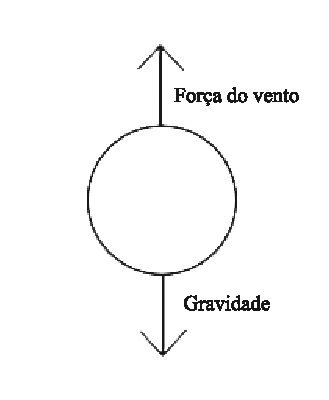
\includegraphics[width=0.3\linewidth, height=0.3\textheight]{pasta1_figuras/forcasatuantes}
	\caption[Forças atuantes na bola]{Forças atuantes na bola}
	\label{fig:forcasatuantes}
\end{figure}



Na figura \ref{fig:forcasatuantes} vemos que há duas forças atuantes na esfera, a gravidade que a puxa para baixo e a força de empuxo gerada pelo vento. Obtemos a seguinte equação do movimento:
\begin{equation}
m \ddot{h}=F=\dfrac{1}{2} \cdot C_a \cdot\rho \cdot A \cdot (v_{ar}- \dot{h})^2-m\cdot g
\end{equation}

onde $m$ é a massa da esfera, $h$ é a posição vertical da esfera no tubo, $\rho$ é a densidade do ar, $A$ é a área da esfera em contato com o fluxo de ar, $v_{ar}$ é a velocidade do ar dentro do tubo e $C_a$ é o coeficiente aerodinâmico da esfera. O coeficiente aerodinâmico depende da velocidade relativa entre a esfera e o vento, mas para as velocidades baixas de vento que estamos utilizando esse valor pode ser considerado constante. Consideramos $\alpha= \dfrac{1}{2} \cdot C_a \cdot \rho \cdot A$:
\begin{equation} \label{eq:modelo}
\ddot{h}=\dfrac{\alpha}{m}\cdot (v_{ar}-\dot{h})^2-g
\end{equation}

\section{Estimação da Velocidade do Vento}

Para criarmos um simulador do sistema descrito anteriormente precisamos saber o valor de $v_{ar}$. Ele determina a velocidade do vento para diferentes valores de tensão e altura da bola. Não foi possível adquirir um sensor de velocidade do ar devido a problemas de localização geológica, portanto, foi necessário usar de engenhosidade para adquirir a velocidade do ar em diversas alturas.


Foram adquiridas diversas bolas de tênis de mesa e se injetou uma mistura de cola e água nelas para aumentar o seu peso. Foram escolhidos 6 pesos diferentes e medidos em balança com precisão de duas casas decimais. Então para cada peso foi medida a tensão necessária para que se alcance as 6 alturas dentro da região de funcionamento do sensor, 10, 20, 30, 40, 50, 60 cm. Tendo medido a altura e a tensão necessária para alcançar as alturas, bastou utilizar a equação \eqref{eq:modelo} fazendo $\ddot{h}=\dot(h)=0$, obtemos a equação \ref{eq:varx} para obter a velocidade do vento relacionada com uma altura e uma tensão.

\begin{equation}\label{eq:varx}
v_{ar}=\sqrt{\dfrac{gm}{\alpha}}
\end{equation}

Na figura \ref{fig:curvavar} vemos a superfície gerada com os dados medidos. E a partir da função dessa superfície geramos a figura \ref{fig:graficovairaltura1}.

\begin{figure}[htb]
	\centering
	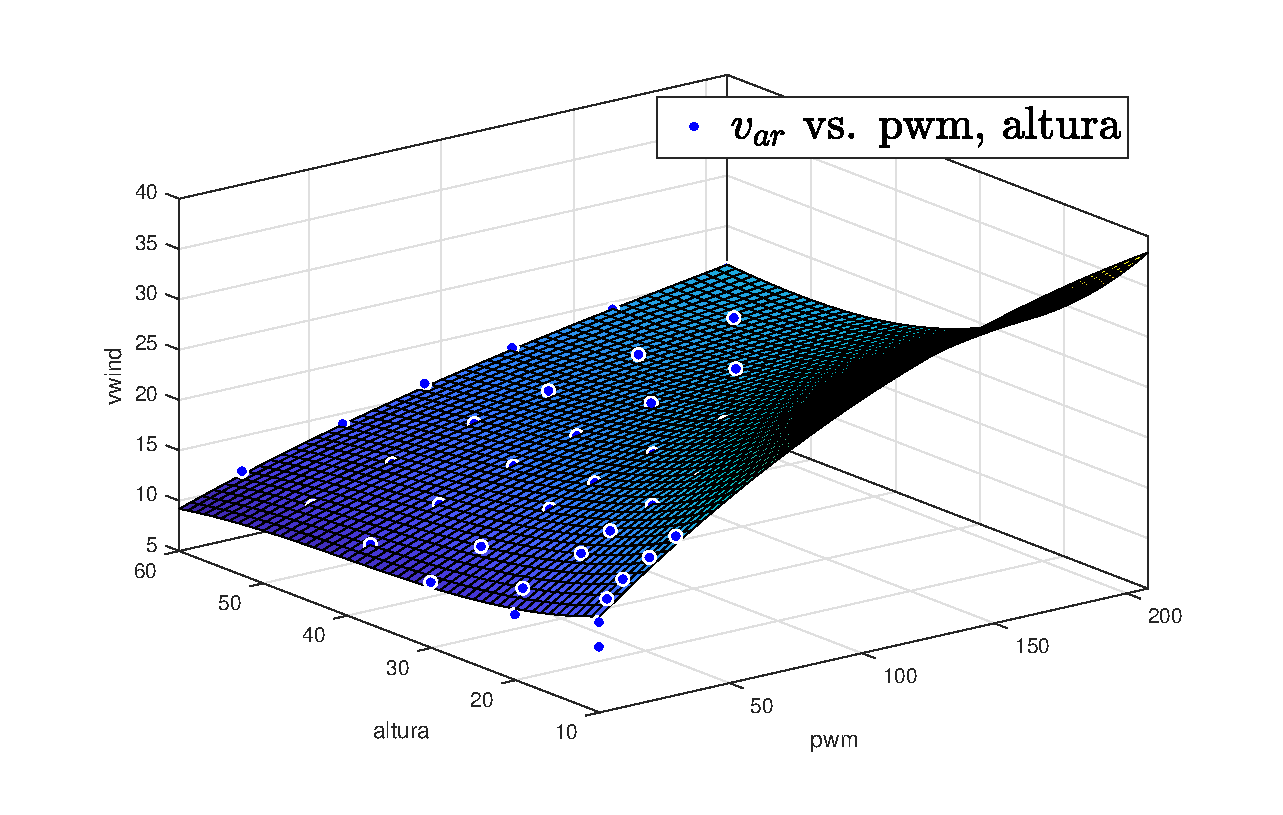
\includegraphics[width=1\linewidth]{pasta1_figuras/curvavar}
	\caption[Superfície de $v_{ar}$ em função de altura e pwm]{Superfície de $v_{ar}$ em função de altura e pwm}
	\label{fig:curvavar}
\end{figure}


\begin{figure}[htb]
	\centering
	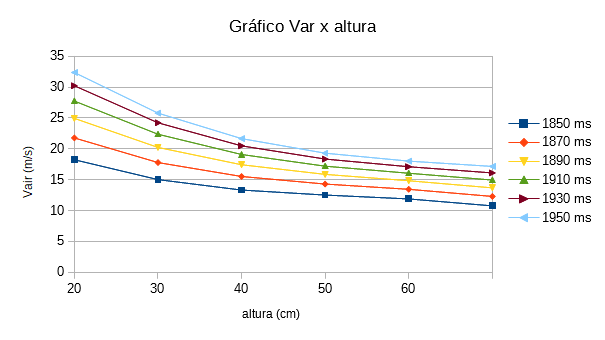
\includegraphics[width=1\linewidth]{grafico_vair_altura}
	\caption[Gráfico $v_{ar}$ x altura]{Gráfico de $v_{ar}$ x altura}
	\label{fig:graficovairaltura1}
\end{figure}

Podemos ver que a figura \ref{fig:graficovairaltura1} lembra um gráfico similar encontrado em \cite{jernigan2009} onde o autor utiliza um sensor de velocidade de vento e mostra uma curva similar, para uma mesma tensão aplicada na turbina quanto mais elevada se encontra a bola menor vai ser a velocidade do ar que se choca com ela.

\section{Simulação do Túnel de Vento no Simulink}

Criamos um modelo de simulação, figura \ref{fig:simulador}, à partir da equação \ref{eq:modelo} e utilizamos os dados adquiridos em \ref{fig:graficovairaltura1} para fazer um ajuste de curva que alimenta o modelo com os valores da velocidade do vento para determinada altura e tensão no motor.

\begin{figure}[htb]
	\centering
	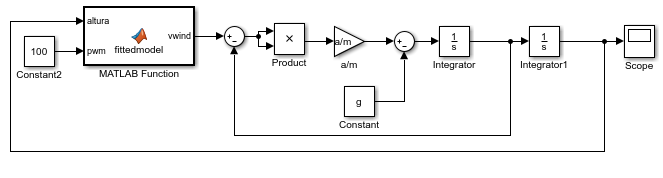
\includegraphics[width=1\linewidth]{simulador}
	\caption[Simulador do túnel de vento]{Simulador do túnel de vento}
	\label{fig:simulador}
\end{figure}

\begin{figure}[htb]
	\centering
	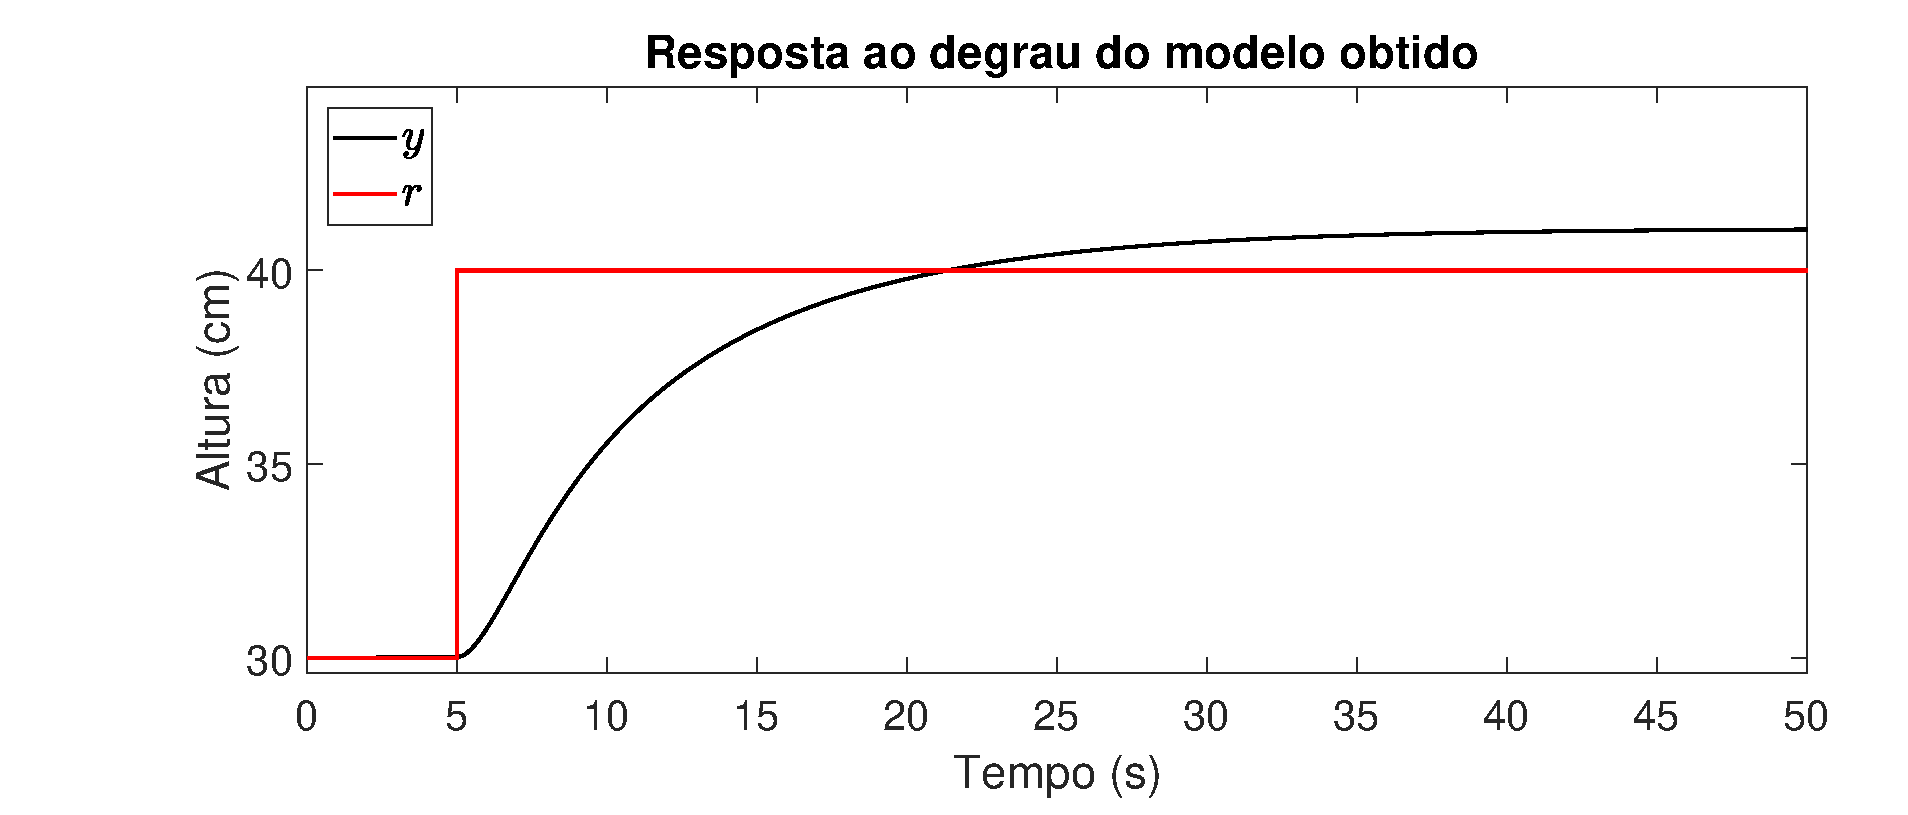
\includegraphics[width=1\linewidth]{pasta1_figuras/step_simul}
	\caption[Resposta ao degrau do simulador]{Resposta ao degrau do simulador}
	\label{fig:stepsimul}
\end{figure}

Na figura \ref{fig:stepsimul} vemos como a resposta do simulador não representa o sistema real. O tempo de estabilização é 10 vezes maior que o tempo do sistema, mas o sobrevalor está condizente com o medido.



% Fim Capítulo

\chapter{Identificação do Túnel de Ar} \label{cap4}
Neste capítulo será explicada a identificação do sistema do túnel de ar. Para fazer a identificação caixa-preta de um sistema é necessário fazer um estudo prévio do funcionamento dele, conhecer entradas e saídas, obter um modelo matemático se possível, mesmo sem ter todos os parâmetros.
\section{Escolha de estrutura}
A escolha da estrutura para identificar um sistema pode ser feita a partir de um modelagem prévia do sistema, mas, em alguns casos a modelagem não é suficiente para obter um modelo adequado. O sistema estudado apresenta certos fenômenos físicos, como o giro da bola devido ao fluxo do ar, que não pudemos modelar.
\subsection{Mínimos Quadrados}\label{s:4mq}
A identificação por Mínimos Quadrados gera um sistema do típo ARX como visto na equação \ref{ARXModel}. A escolha da estrutura neste caso se dá escolhendo uma quantidade de regressores da saída e uma quantidade de regressores da entrada. Tendo em vista que o modelo matemático encontrado em \ref{eq:modelo} não é capaz de prever completamente o funcionamento do sistema foi necessário escolher um método diferente da análise do modelo.


Para a escolha da estrutura do modelo do sistema foi feito o seguinte procedimento:
\begin{enumerate}
	\item Escolher uma quantidade de regressores de $y$
	\item Escolher uma quantidade de regressores de $u$
	\item Fazer a identificação por Mínimos Quadrados com os regressores de $y$ e $u$
	\item Analisar a autocorrelação dos resíduos $\xi=y-\Psi \hat{\theta}$
\end{enumerate}

Este procedimento foi repetido para valores de 1 a 10 para ambos os regressores e ao final se identificou que a melhor ordem para os regressores foi com 9 polos e 8 zeros. Na figura \ref{fig:autocorrelacao98} a auto correlação dos resíduos do sistema identificado.

\begin{figure}[H]
	\centering
	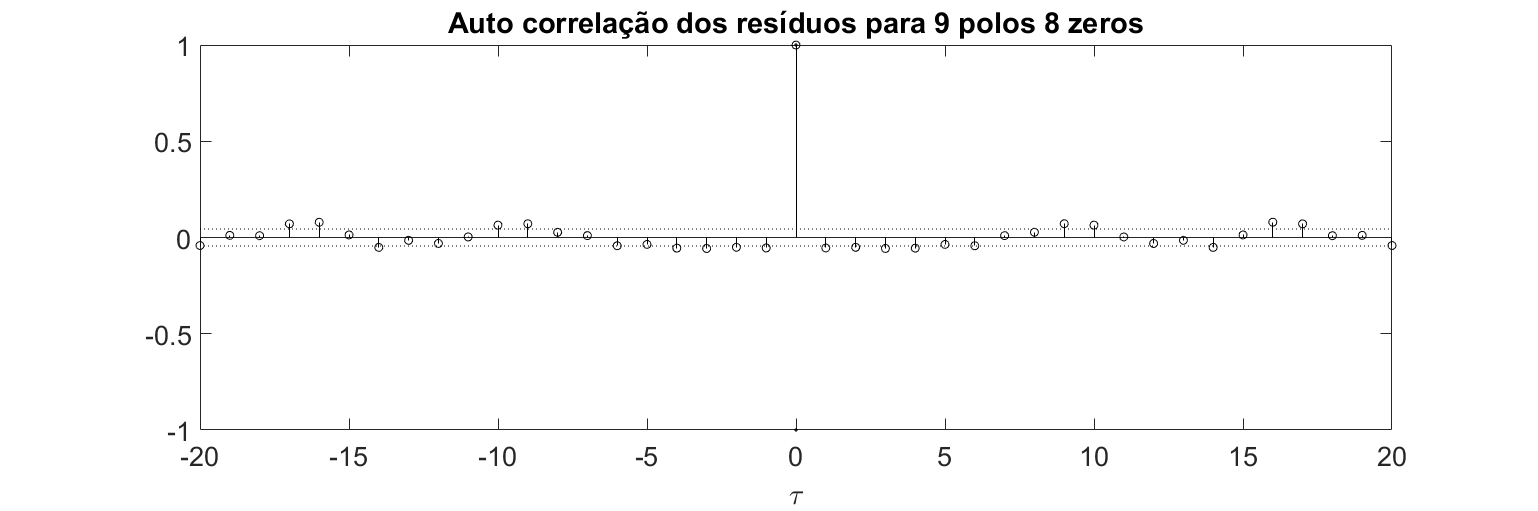
\includegraphics[width=1.1\linewidth]{autocorrelacao98}
	\caption[Autocorrelação dos resíduos para sistema com 9 polos e 8 zeros]{Autocorrelação dos resíduos para sistema com 9 polos e 8 zeros}
	\label{fig:autocorrelacao98}
\end{figure}

\subsection{Subespaços}\label{s:4subespacos}
A identificação por Subespaços gera um sistema em espaço de estados como visto na equação \ref{eq:ss}. Neste tipo de identificação a escolha da estrutura é feita decidindo a ordem do sistema e a ordem da matriz em blocos de Hankel. E similarmente ao procedimento feito na seção \ref{s:4mq} foram variadas as ordens do sistema e da matriz em blocos de Hankel.
Foi escolhida ordem 3 para o sistema e ordem 15 para a matriz em blocos de Hankel usada para identificar o sistema. Vemos na figura \ref{fig:autocorrelacao315} a auto correlação dos resíduos do sistema identificado.

\begin{figure}[H]
	\centering
	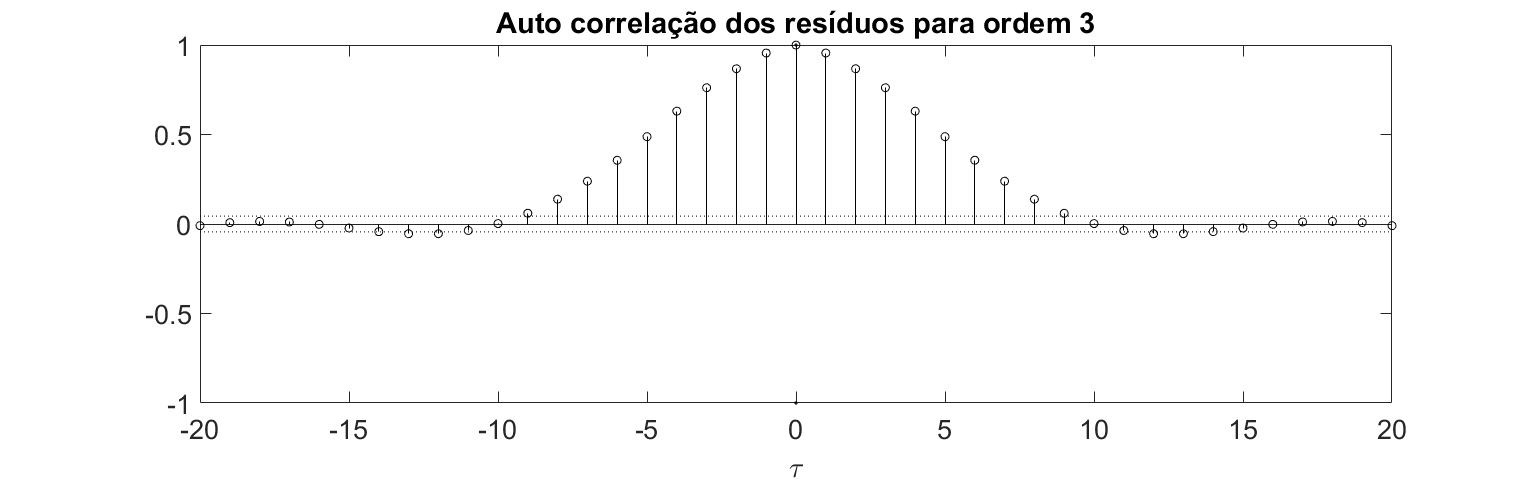
\includegraphics[width=1.1\linewidth]{autocorrelacao315}
	\caption[Autocorrelação dos resíduos para sistema de ordem 3]{Autocorrelação dos resíduos para sistema de ordem 3 identificado com matriz em blocos de Hankel ordem 15}
	\label{fig:autocorrelacao315}
\end{figure}

\section{Experimento}\label{s:4experimento}
O experimento para identificação precisa de um sinal adequado para que a resposta à ele consiga mostrar a dinâmica do sistema. Para tanto foi gerado um sinal PRBS (sinal binário pseudo aleatório) que é suficientemente adequado para extrair a dinâmica do sistema. O sinal é aplicado ao sistema através do Arduino e os sinais são medidos com um tempo de amostragem de 50 ms.
\begin{figure}[H]
	\centering
	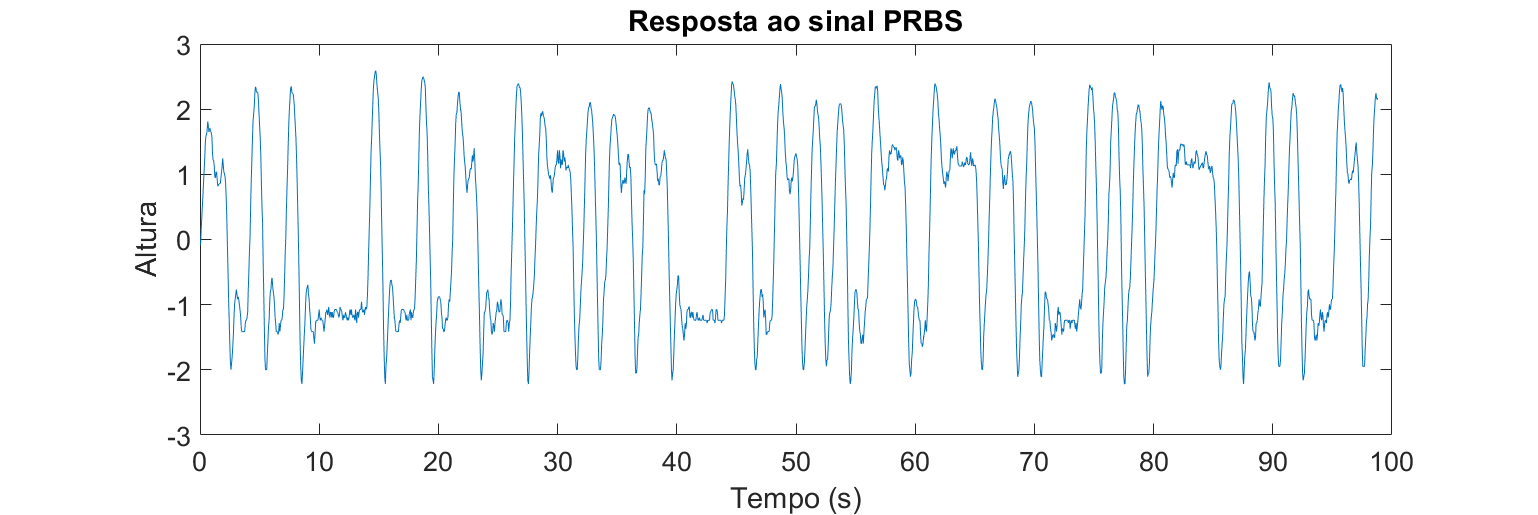
\includegraphics[width=1.1\linewidth]{sinalprbsid}
	\caption[Gráfico da saída PRBS]{Gráfico da saída ao aplicar o sinal PRBS com tempo de amostragem de 50ms}
	\label{fig:sinalprbsid}
\end{figure}

A figura \ref{fig:sinalprbsid} mostra a resposta do sistema ao sinal PRBS que foi aplicado ao sistema, podemos ver seções do teste onde o sinal possibilitou que o sistema tivesse algum tempo para estabilizar como em torno dos 10 e 80 segundos,e em outros o sistema é posto em movimento.

\section{Estimação}\label{s:4estimacao}

Com a resposta do sistema e o sinal de entrada podemos então identificar o sistema.
\subsection{Mínimos Quadrados}\label{s:4estmq}
Para fazer a identificação por mínimos quadrados geramos a matriz de regressores $\psi$ da equação \ref{eq:regressores} e usamos a equação \ref{eq:MQ} para obter os coeficientes dos regressores. Obtemos um sistema com o seguinte modelo ARX:


\commentib{tentei alinhar essas equações mas não enconrei como}
\begin{equation}
y[k]= A[k]+ B[k] 
\end{equation}
\begin{equation}
\begin{aligned}
A[k]=- 1.463\cdot U[k-1] + 0.6593 \cdot U[k-2] - 0.4703\cdot U[k-3] + 0.3195\cdot U[k-4] + 0.1436\cdot U[k-5]\\- 0.1106\cdot U[k-6] + 0.07184 \cdot U[k-7] - 0.0766\cdot U[k-8] + 0.02136 \cdot U[k-9]
\end{aligned}
\end{equation}
\begin{equation}
\begin{aligned}
B[k]=-0.004773\cdot U[k-1] - 0.002941\cdot U[k-2] + 0.01512\cdot U[k-3] + 0.01026\cdot U[k-4]\\ + 0.04134\cdot U[k-5] + 0.01709\cdot U[k-6] + 0.003757\cdot U[k-7]   + 0.0386 U[k-8]
\end{aligned}
\end{equation}

A resposta ao degrau do sistema identificado é visto na figura \ref{fig:respostadegrauarx}.

\begin{figure}[H]
	\centering
	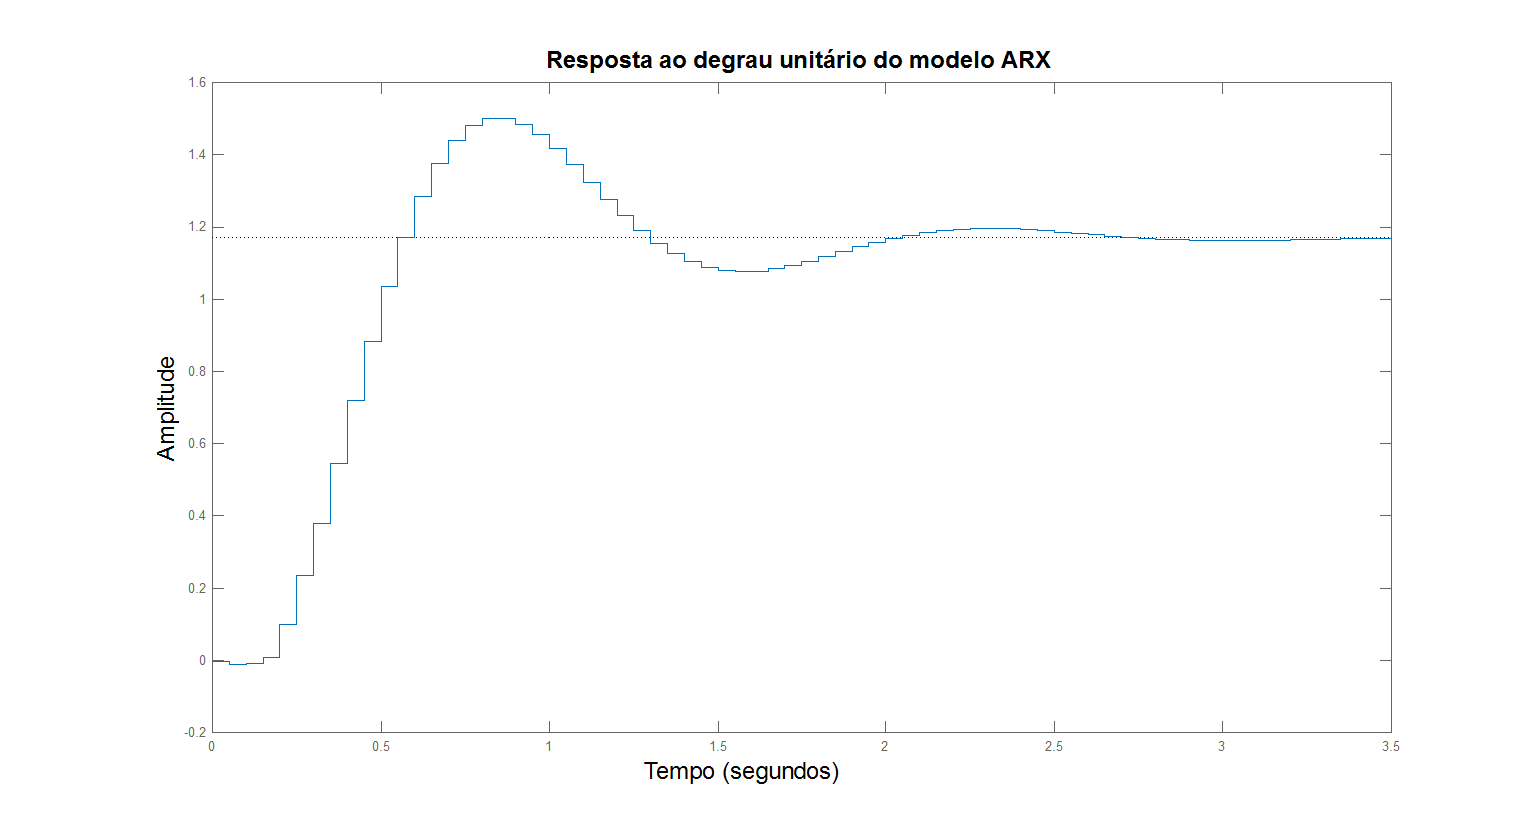
\includegraphics[width=1\linewidth]{respostadegrauarx}
	\caption[Resposta ao degrau do modelo ARX]{Resposta ao degrau unitário do modelo ARX identificado}
	\label{fig:respostadegrauarx}
\end{figure}

\subsection{Subespaços}\label{s:4estsub}

Para identificar o sistema usando subespaços utilizamos o algoritmo mostrado na seção \ref{s:subalgoritmos} com uma matriz em blocos de Hankel de ordem 15 para encontrar um sistema de ordem 3. Identificamos o seguinte modelo com o formato da equação \ref{eq:ss}:

\begin{equation}
A=\begin{bmatrix}
0.9761  &  0.1933 &  -0.0438\\
-0.1817  &  0.9841  & -0.1489\\
0.0840  &  0.3107  &  0.6994
\end{bmatrix}
\end{equation}

\begin{equation}
B=\begin{bmatrix}
0.1466\\
0.2515\\
0.8460
\end{bmatrix}
\end{equation}
\begin{equation}
C=\begin{bmatrix}
-1.0104 &  -0.3354 &   0.2496
\end{bmatrix}
\end{equation}
\begin{equation}
D=\begin{bmatrix}
0.0010
\end{bmatrix}
\end{equation}
Na figura \ref{fig:respostadegrausub} vemos a resposta ao degrau do sistema identificado, e, ao comparar com a resposta ao degrau do sistema ARX identificado, figura \ref{fig:respostadegrauarx}, podemos ver que ambos são sistemas estáveis e subamortecidos, apesar de apresentarem um tempo de assentamento diferente.

\begin{figure}[H]
	\centering
	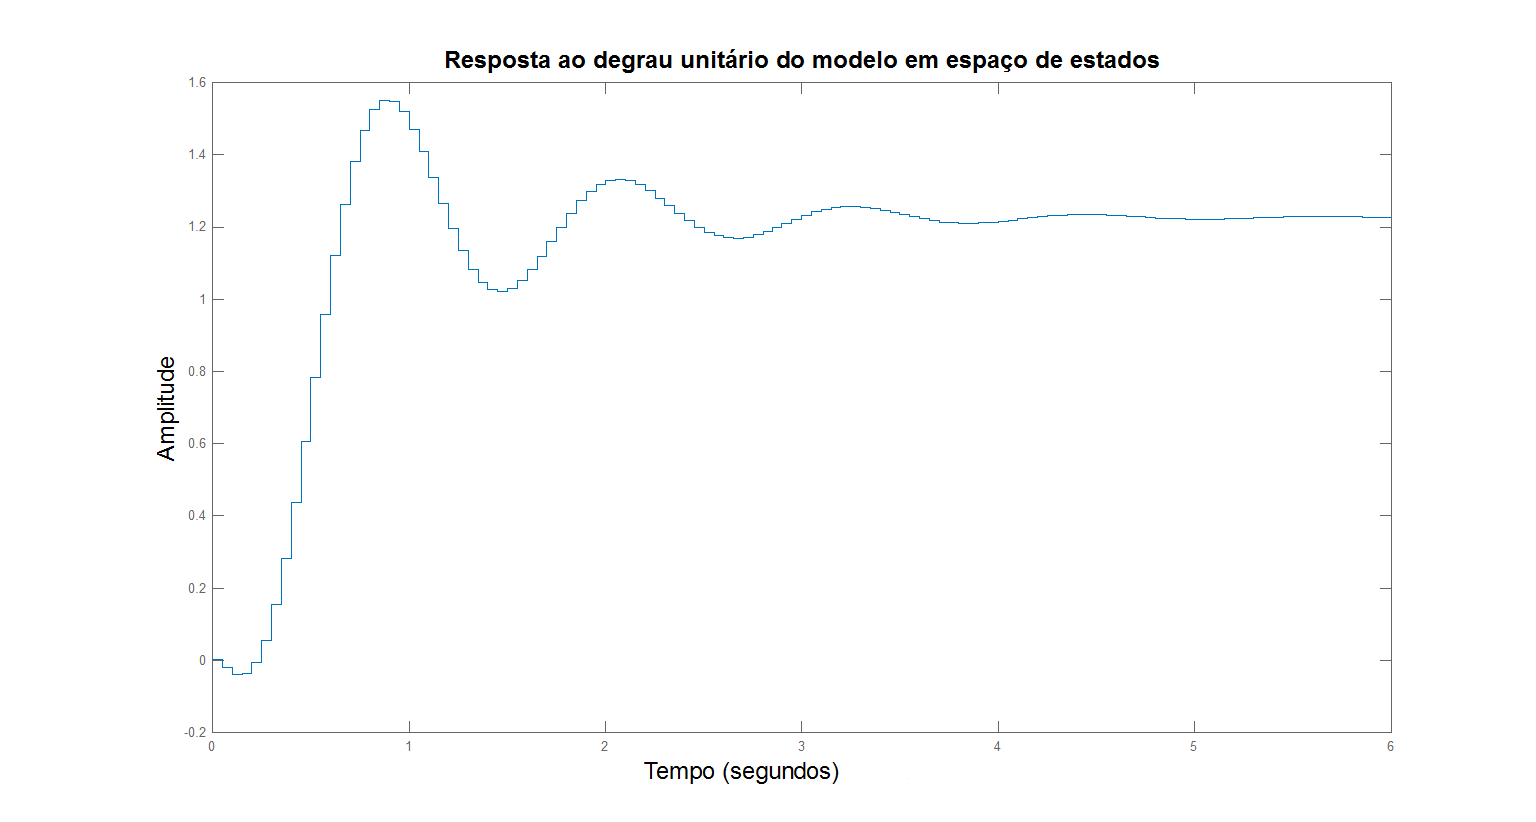
\includegraphics[width=1\linewidth]{respostadegrausub}
	\caption[Resposta ao degrau do modelo em espaço de estados]{Resposta ao degrau unitário do modelo em espaço de estados identificado}
	\label{fig:respostadegrausub}
\end{figure}

\section{Validação}\label{s4:val}
Ao identificar um sistema precisamos validar o modelo obtido para garantir que ele é adequado para representar o sistema real. Para isso fazemos uma análise da auto correlação dos resíduos $\xi=y-\Psi \hat{\theta}$ para o ARX e $\xi=y-y_{sim}$ para o espaço de estados. Como vemos nas figuras \ref{fig:autocorrelacao98} e \ref{fig:autocorrelacao315} os resíduos do modelo ARX são muito menos correlacionados do que os do modelo em espaço de estados. Isso acontece porque para o modelo ARX estamos analisando os seus regressores com a matriz $\Psi$ que os gera, o que retorna uma resposta muito mais próxima do sistema. Já para o espaço de estados estamos analisando a simulação do sistema, que apresenta pequenas diferenças em relação ao sistema real, como a ausência de ruído.


Ambos os sistemas, no entanto, apresentam uma análise de ruídos satisfatória e uma resposta ao sinal PRBS muito próxima do sistema real.



% Fim Capítulo
\chapter{Projeto de Controlador com Alocação de Polos Baseado nos Modelos Identificados} \label{cap5}
Com o sistema identificado, podemos finalmente controlá-lo, faremos isso através de realimentação de estados para os quatro modelos identificados.

\section{Alocação de Polos com Realimentação de Estados}
Para fazer o controle por realimentação de estados precisamos passar os 3 modelos ARX obtidos para modelos em espaço de estados Fazemos isso usando a função do Matlab tf2ss, onde entramos com o nominador e denominador do modelo ARX e a função nos retorna as matrizes A, B, C e D do sistema em espaço de estados. 


Queremos controlar os 4 modelos fazendo alocação de polos através da realimentação de estados. Projetamos os controladores para que atendam como requisitos um sobrevalor menor que 4\% do valor final e tempo de assentamento menor que 2 segundos quando recebe um entrada do tipo degrau unitário.

\subsection{Modelo $SUB1$}

Para atender os requisitos de tempo de assentamento $t_s<2 ~s$ e sobrevalor máximo de $ovs<4\%$ calculamos os valores de $\zeta$ e $\omega_n$ usados na equação característica de um sistema de segunda ordem \eqref{eq:mso}, usando as equações \eqref{eq:ovs} e \eqref{eq:ts}.

\begin{equation}\label{eq:mso}
G(s)=\dfrac{\omega_n^2}{s^2+2 \zeta \omega_n  s+ \omega_n^2}
\end{equation}

\begin{equation}\label{eq:ovs}
ovs=e^{\dfrac{\zeta \pi}{\sqrt{1-\zeta^2}}}<4\%
\end{equation}

\begin{equation}\label{eq:ts}
t_s=\dfrac{4}{\zeta \omega_n}<2~s
\end{equation}

Encontramos $\zeta>0.7157$ e $\omega_n>2.7945$, e escolhemos os valores de $\zeta=0.9$ e $\omega_n=4$. Ao aplicar esses valores na equação \eqref{eq:mso} obtemos os polos que precisamos alocar no domínio s, $s_1=-3.6000 + 1.7436i$ e $s_2=-3.6000 - 1.7436i$. Como o modelo $SUB'$ tem ordem 3 precisamos de um terceiro polo distante da parte real dos anteriores, escolhemos $s_3=-8$. Passamos os três polos para o domínio z e obtemos $z_1=0.8321 + 0.0727i$, $z_2=0.8321 - 0.0727i$ e $z_3=0.6703$. 


Para fazer a alocação de polos usamos a equação de Lyapunov
\eqref{eq:lyapeq}:
\begin{equation}\label{eq:lyapeq}
(A-B\bar{k})T=TF
\end{equation}

Onde $A$ e $B$ são matrizes do sistema, $\bar{k}$ é um vetor arbitrário escolhido de forma que o par $F$ e $\bar{k}$ seja observável, $F$ é uma matriz em blocos diagonais com os polos que se deseja alocar e $k=\bar{k}*T^{-1}$ nos retorna o vetor de realimentação de estados $k$. Obtemos $k=[0.7552,~0.2637,~0.1750]$ Com essa realimentação de estados obtemos a seguinte resposta ao degrau:

\begin{figure}[H]
	\centering
	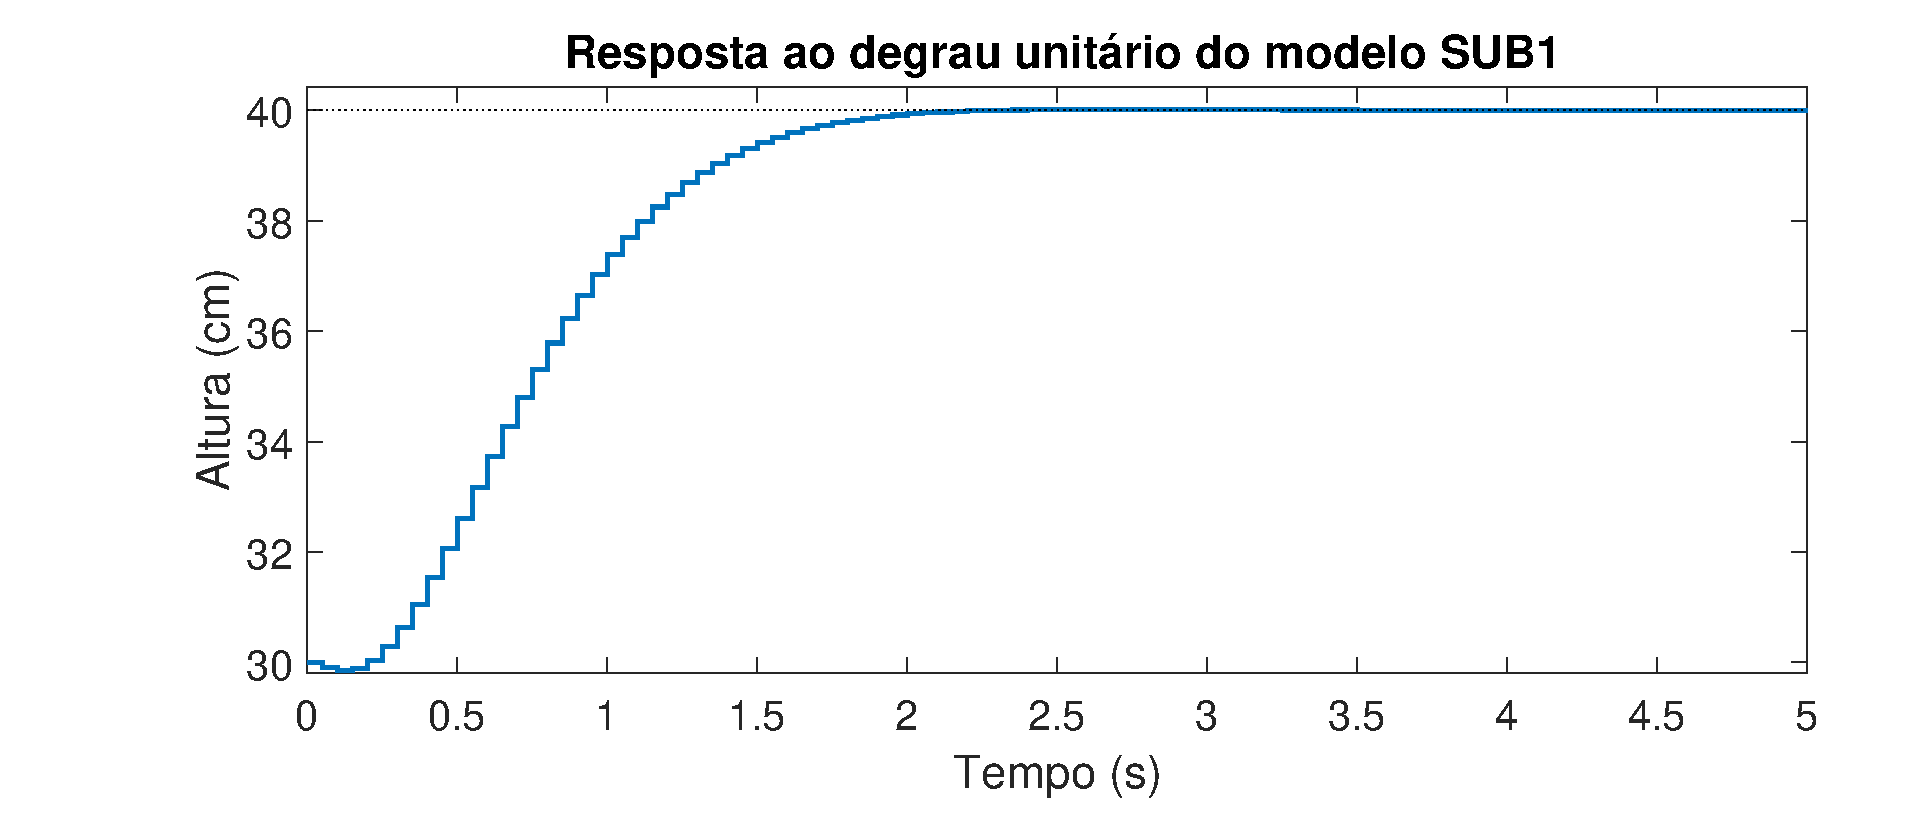
\includegraphics[width=1\linewidth]{respostadegrausub1c}
	\caption[Resposta ao degrau unitário do modelo $SUB1$ controlado]{Resposta ao degrau unitário do modelo simulado $SUB1$ controlado}
	\label{fig:respostadegrausub1c}
\end{figure}


A resposta ao degrau do sistema como vista na figura \ref{fig:respostadegrausub1c} apresenta um tempo de assentamento de 1.8 segundos e um sobrevalor de 0.14\%.

\subsection{Modelo $ARX1$}

Para o modelo $ARX1$ escolhemos os valores de $\zeta=0.9$ e $\omega_n=7$. Ao aplicar esses valores na equação \eqref{eq:mso} obtemos os polos que precisamos alocar no domínio s, $s_1=-6.3000 + 3.0512i$ e $s_2=-6.3000 - 3.0512i$, para o polo distante alocamos $s_3=-15$. Que no domínio z são $z_1=0.7213 + 0.1109i$, $z_2=0.7213 - 0.1109i$ e $z_3=0.4966$. Repetimos o mesmo procedimento de alocação de polos usado no modelo $SUB1$ e obtemos $k=[-0.2840,~0.6313,~-0.3481]$.


O sistema realimentado tem a seguinte resposta ao degrau:

\begin{figure}[H]
	\centering
	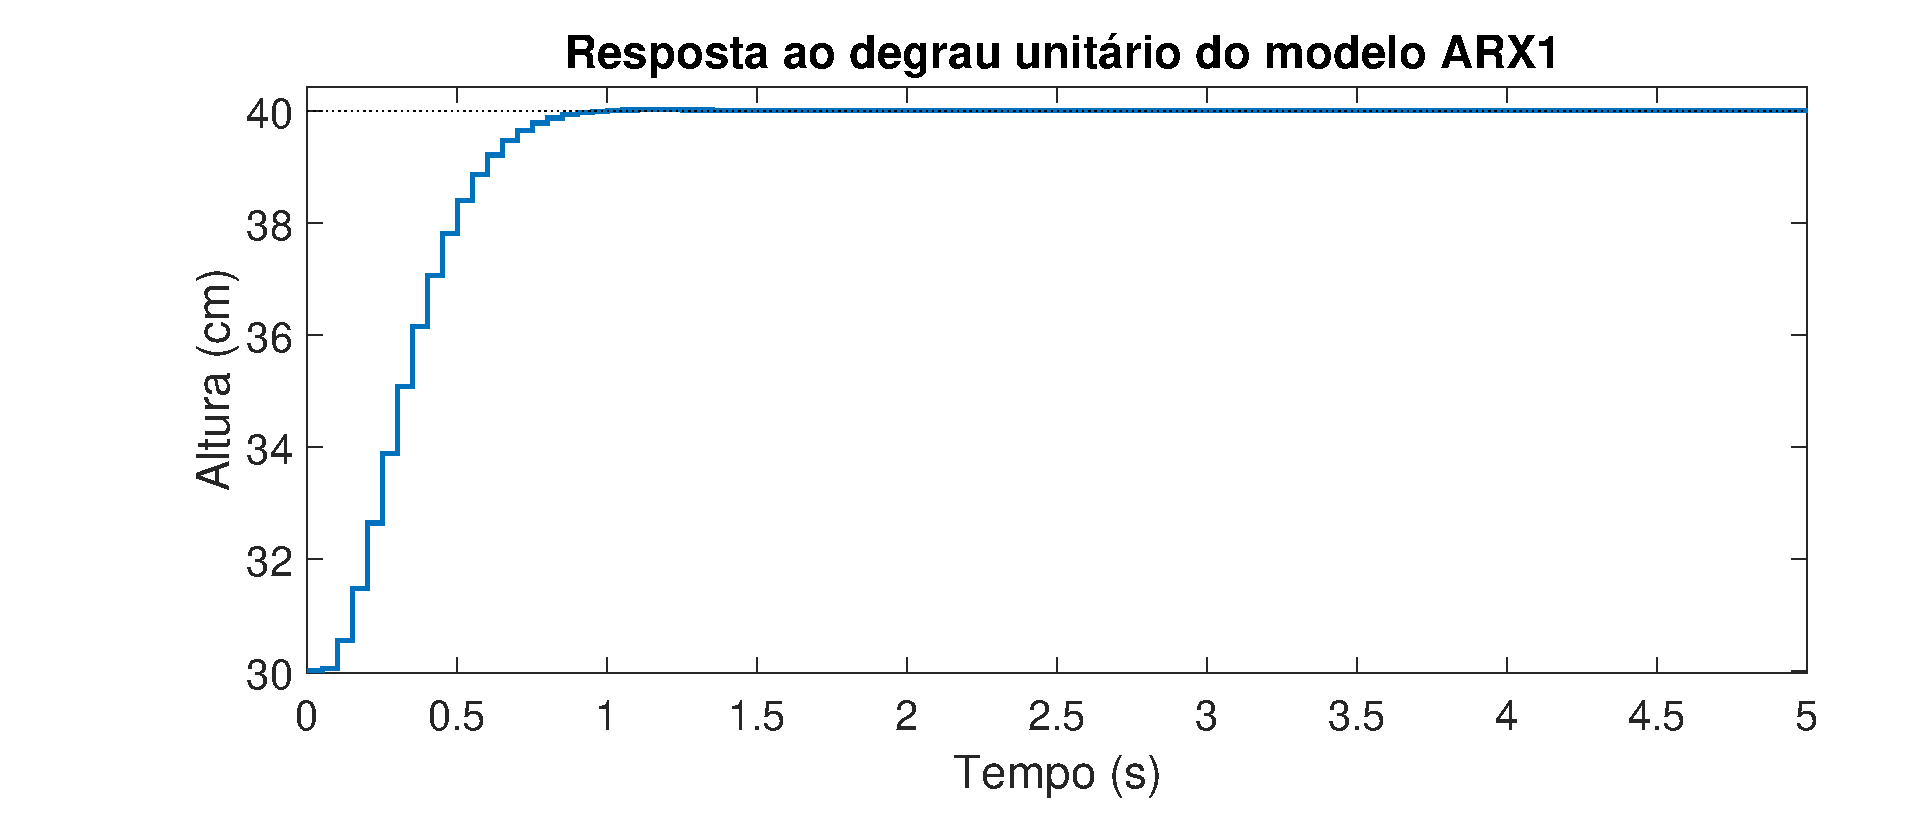
\includegraphics[width=1\linewidth]{respostadegrauarx1c}
	\caption[Resposta ao degrau do modelo simulado $ARX1$ controlado]{Resposta ao degrau do modelo simulado $ARX1$ controlado}
	\label{fig:respostadegrauarx1c}
\end{figure}


A resposta ao degrau da figura \ref{fig:respostadegrauarx1c} apresenta um tempo de assentamento de 0.8 segundos e um sobrevalor de 0,125\%.

\subsection{Modelo $ARX2$}
Para o modelo $ARX2$ escolhemos $\zeta=0.9$ e $\omega_n=9$. Aplicando na equação \eqref{eq:mso} obtemos os polos para alocar no domínio s, $s_1=-8.1000 + 3.9230i$ e $s_2=-8.1000 - 3.9230i$. Este modelo ainda tem 3 polos extras que devem ser alocados distantes dos polos $s_1$ e $s_2$, escolhemos $s_3=-14$, $s4=-14.1$ e $s_5=-14.2$. Que no domínio z são $z_1=0.6542 + 0.1300i$, $z_2=0.6542 - 0.1300i$, $z_3=0.4966$, $z_4=0.4941$ e $z_5=0.4916$. Fazemos a alocaçao de polos da mesma forma que foi feita para o modelo $SUB1$ obtemos $k=[-1.2401,~2.3566,~-1.2062,~-0.0018,~0.0360]$.

O sistema controlado tem a seguinte resposta ao degrau unitário:

\begin{figure}[H]
	\centering
	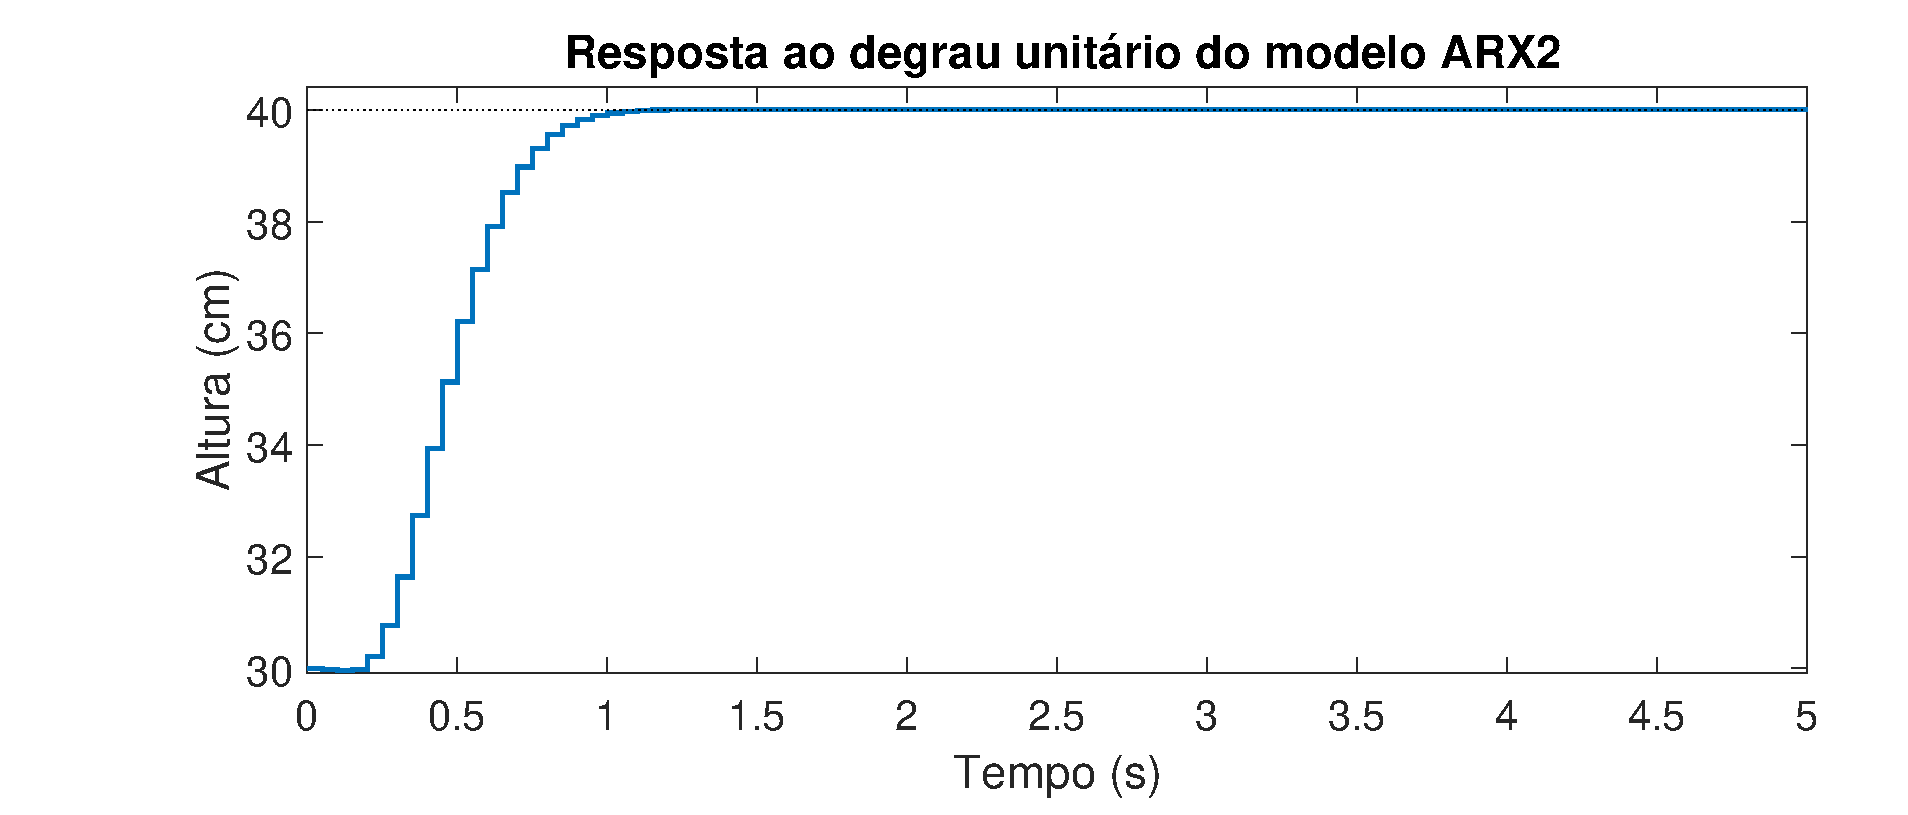
\includegraphics[width=1\linewidth]{respostadegrauarx2c}
	\caption[Resposta ao degrau do modelo $ARX2$]{Resposta ao degrau do modelo simulado $ARX2$ controlado}
	\label{fig:respostadegrauarx2c}
\end{figure}

Vemos na figura \ref{fig:respostadegrauarx2c} que a resposta ao degrau unitário do sistema controlado tem tempo de assentamento de 0.9 segundos e sobrevalor de 0.0326\%


\subsection{Modelo $ARXsim$}

Para o modelo $ARXsim$ escolhemos $\zeta=0.9$ e $\omega_n=9$. Aplicados na equação\eqref{eq:mso} obtemos os polos no domínio s, $s_1=-3.6000 + 1.7436i$ e $s_2=-3.6000 - 1.7436i$, e escolhemos o polo distante $s_3=-8$. No domínio z os polos são $z_1=0.8321 + 0.0727i$, $z_2=0.8321 - 0.0727i$ e $z_3=0.4966$. Fazemos a alocação de polos como foi feito para o modelo $SUB1$ e obtemos $k=[-1.1499,~1.0710,~0.0876]$.
O sistema controlado tem a seguinte resposta ao degrau unitário:

\begin{figure}[H]
	\centering
	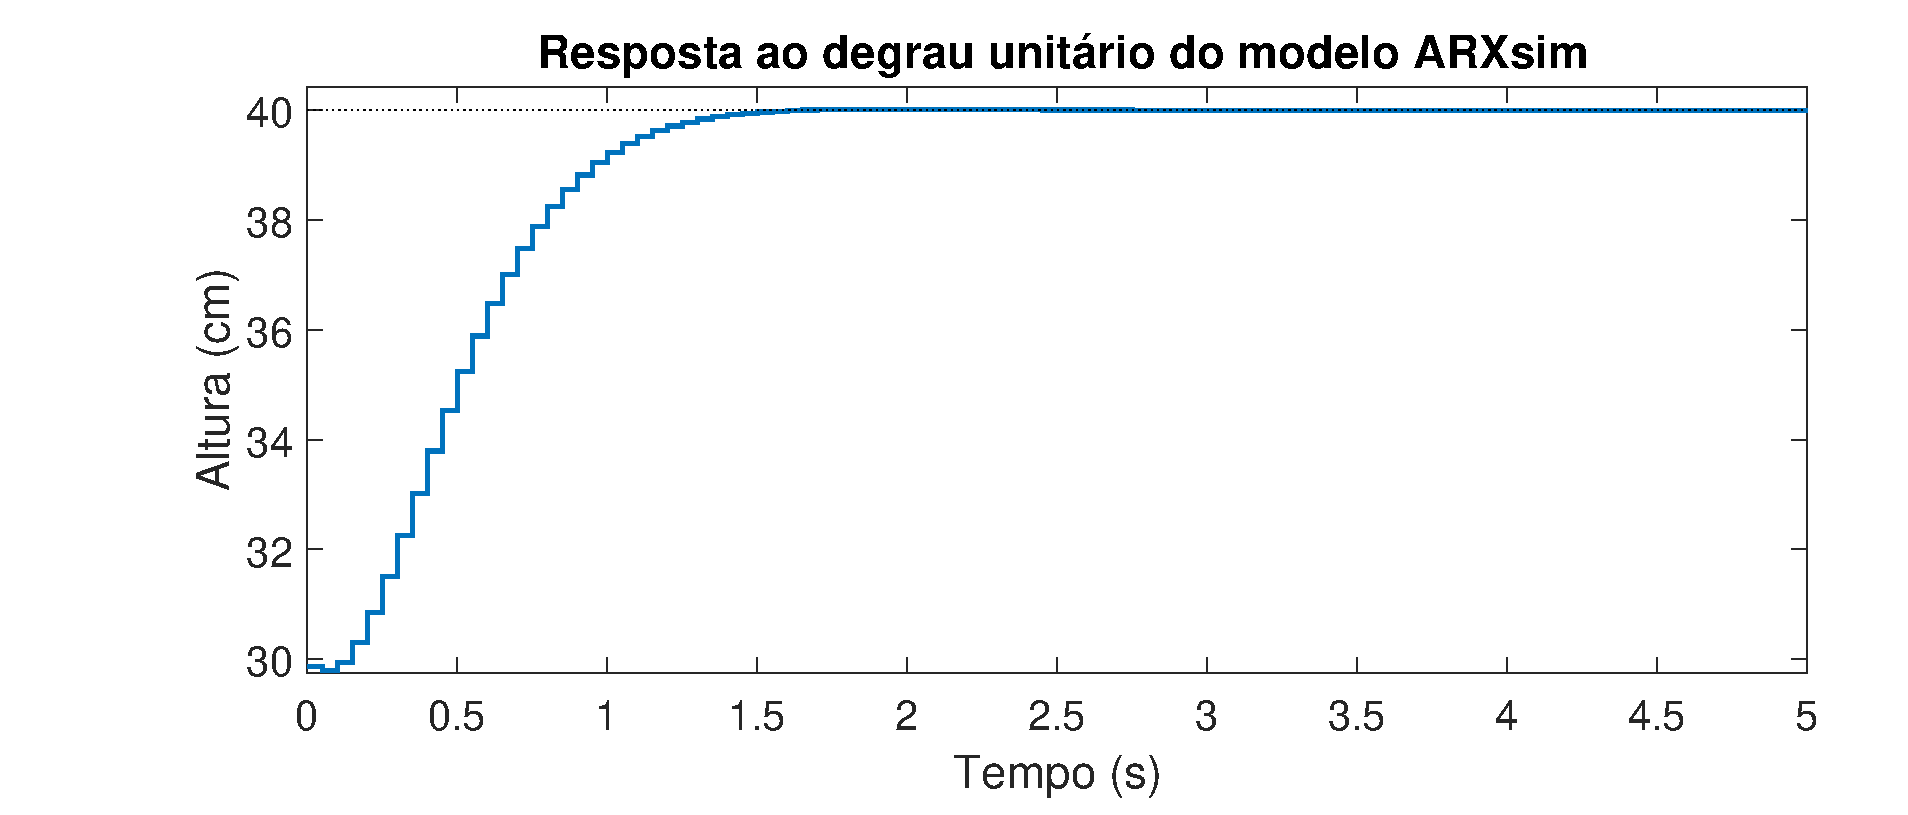
\includegraphics[width=1\linewidth]{respostadegrauarxsimc}
	\caption[Resposta ao degrau do modelo simulado $ARXsim$]{Resposta ao degrau do modelo simulado $ARXsim$ controlado}
	\label{fig:respostadegrauarxsimc}
\end{figure}

Vemos na figura \ref{fig:respostadegrauarxsimc} que a resposta ao degrau unitário do sistema controlado tem tempo de assentamento de 1.3 segundos e máximo sobrevalor de 0.1487\%.


\section{Projeto do Estimador de Estados}
Para realizar um controlador por realimentação de estados precisamos ser capazes de medir todos os estados do nosso modelo a cada tempo de amostragem. O nosso sistema, no entanto, não tem sensores para medir cada um dos estados necessários, a única medida disponível é a saída do sistema na forma da altura da bola. Portanto, precisamos implementar um estimador de estados para cada um dos controladores projetados na subseção anterior.

\subsection{Modelo $SUB1$}
Um estimador de estados é projetado de forma similar ao controlador por realimentação de estados, precisamos escolher polos adequados para que o estimador funcione da forma correta. A forma mais simples de escolher esses polos é fazer com que eles reajam mais rápido que o sistema à entrada recebida, conseguimos isso multiplicando a parte real dos polos no domínio s por um número para que sejam mais rápidos. 


Projetamos o estimador de estados com os seguintes polos $z_1=0.1647 + 0.0144i$, $z_2=0.1647 - 0.0144i$ e $z_3=0.0183$ e obtemos o ganho do estimador $L=[3.5436,~-7.2192,~13.9077]^T$. Nas figuras \ref{fig:estimadorsub1} e \ref{fig:stepestsub1} vemos como uma simulação do sistema se comporta.

\begin{figure}[H]
	\centering
	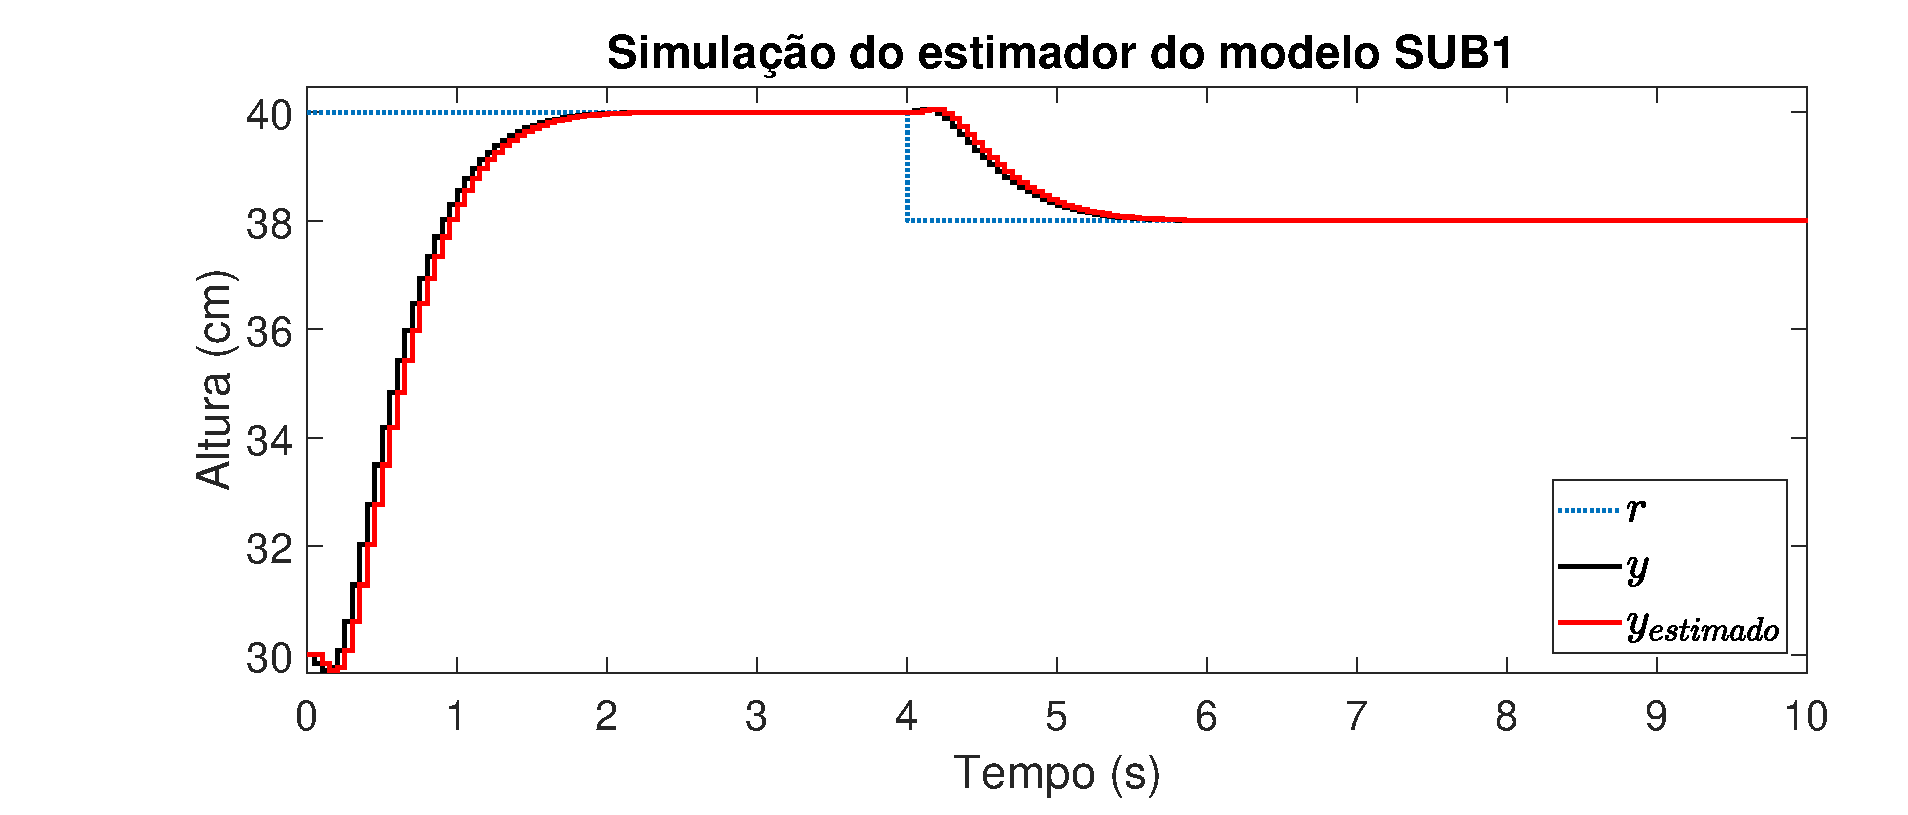
\includegraphics[width=1\linewidth]{estimadorsub1}
	\caption[Simulação do estimador do modelo $SUB1$]{Simulação do estimador do modelo $SUB1$}
	\label{fig:estimadorsub1}
\end{figure}

\begin{figure}[H]
	\centering
	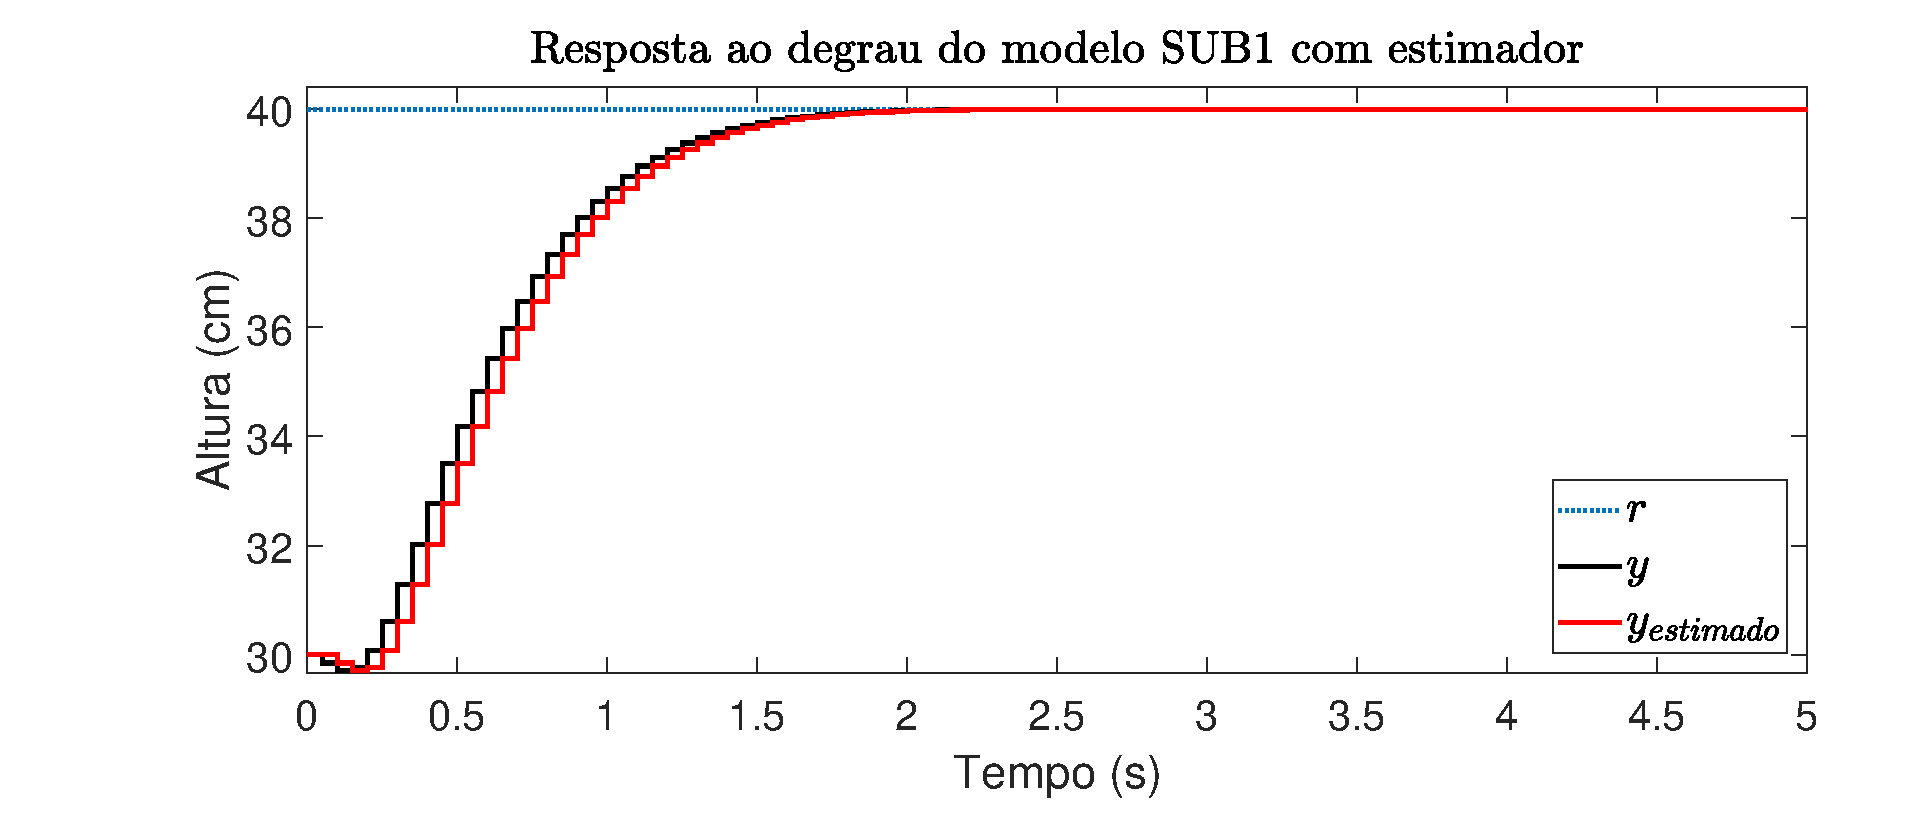
\includegraphics[width=1\linewidth]{stepestsub1}
	\caption[Resposta ao degrau do modelo $SUB1$ controlado com observador]{Resposta ao degrau do modelo $SUB1$ controlado com observador}
	\label{fig:stepestsub1}
\end{figure}



\subsection{Modelo $ARX1$}
Para o estimador do modelo $ARX1$ alocamos os polos em $z_1=0.0309 + 0.0048i$, $z_2=0.0309 - 0.0048i$ e $z_3=0.0003$. Obtemos o ganho do estimador $L=[33.9534,~26.6709,~16.6024]^T$. Nas figuras \ref{fig:estimadorarx1} e \ref{fig:stepestarx1} vemos como uma simulação do sistema se comporta.

\begin{figure}[H]
	\centering
	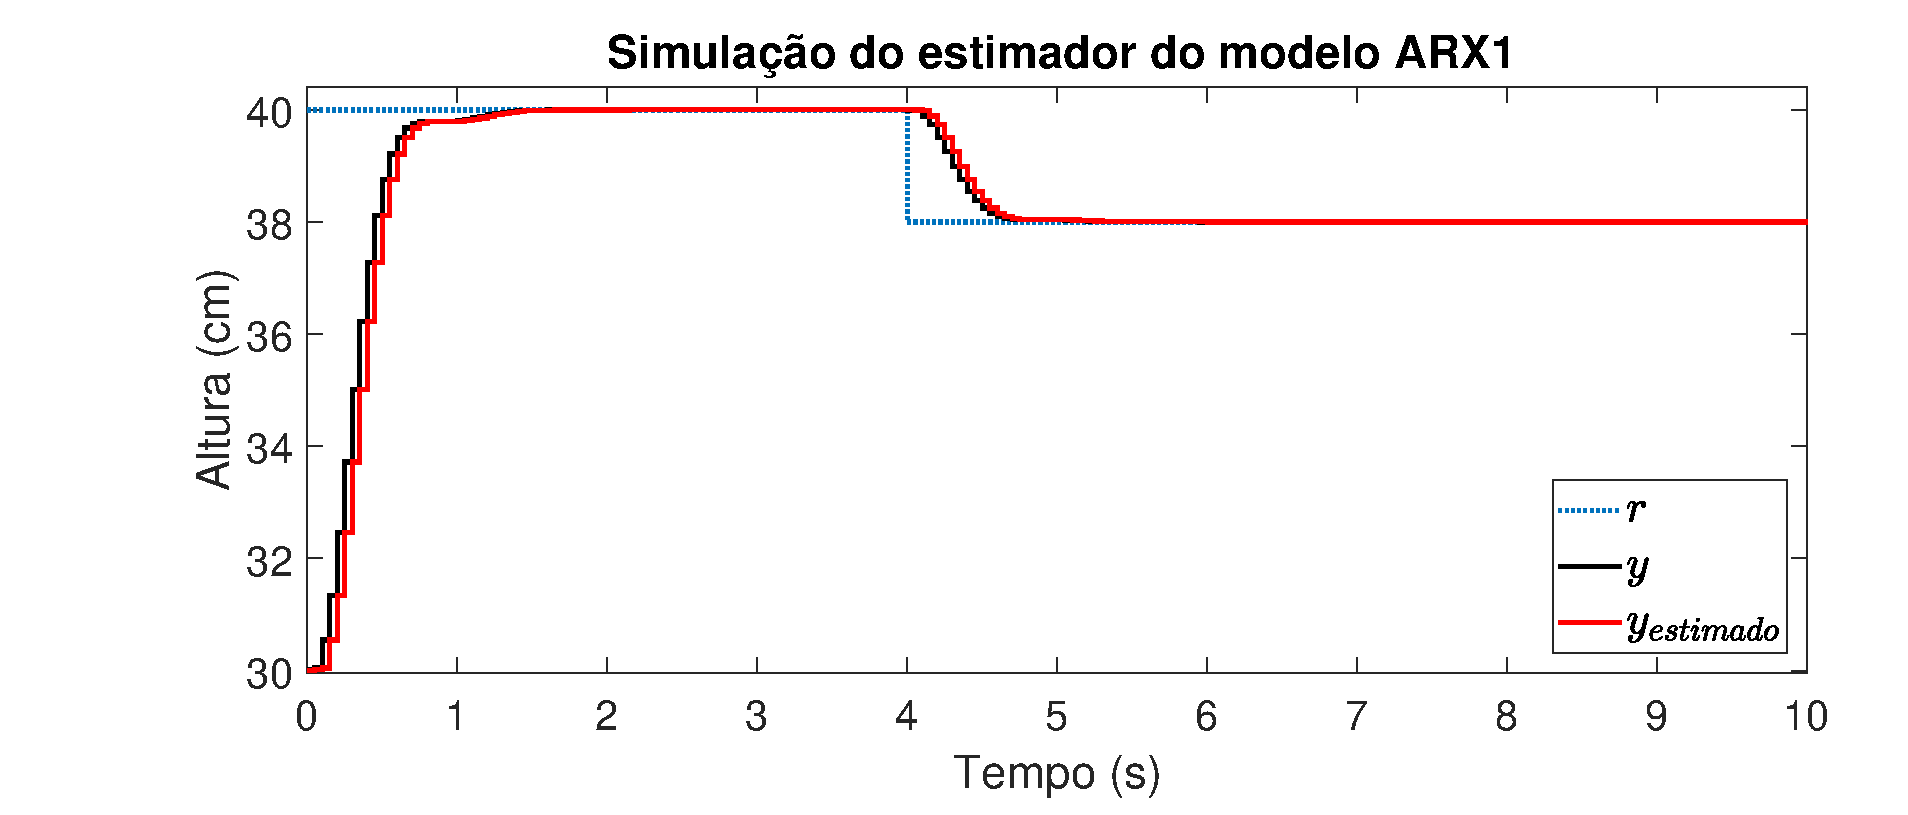
\includegraphics[width=1\linewidth]{estimadorarx1}
	\caption[Simulação do estimador do modelo $ARX1$]{Simulação do estimador do modelo $ARX1$}
	\label{fig:estimadorarx1}
\end{figure}

\begin{figure}[H]
	\centering
	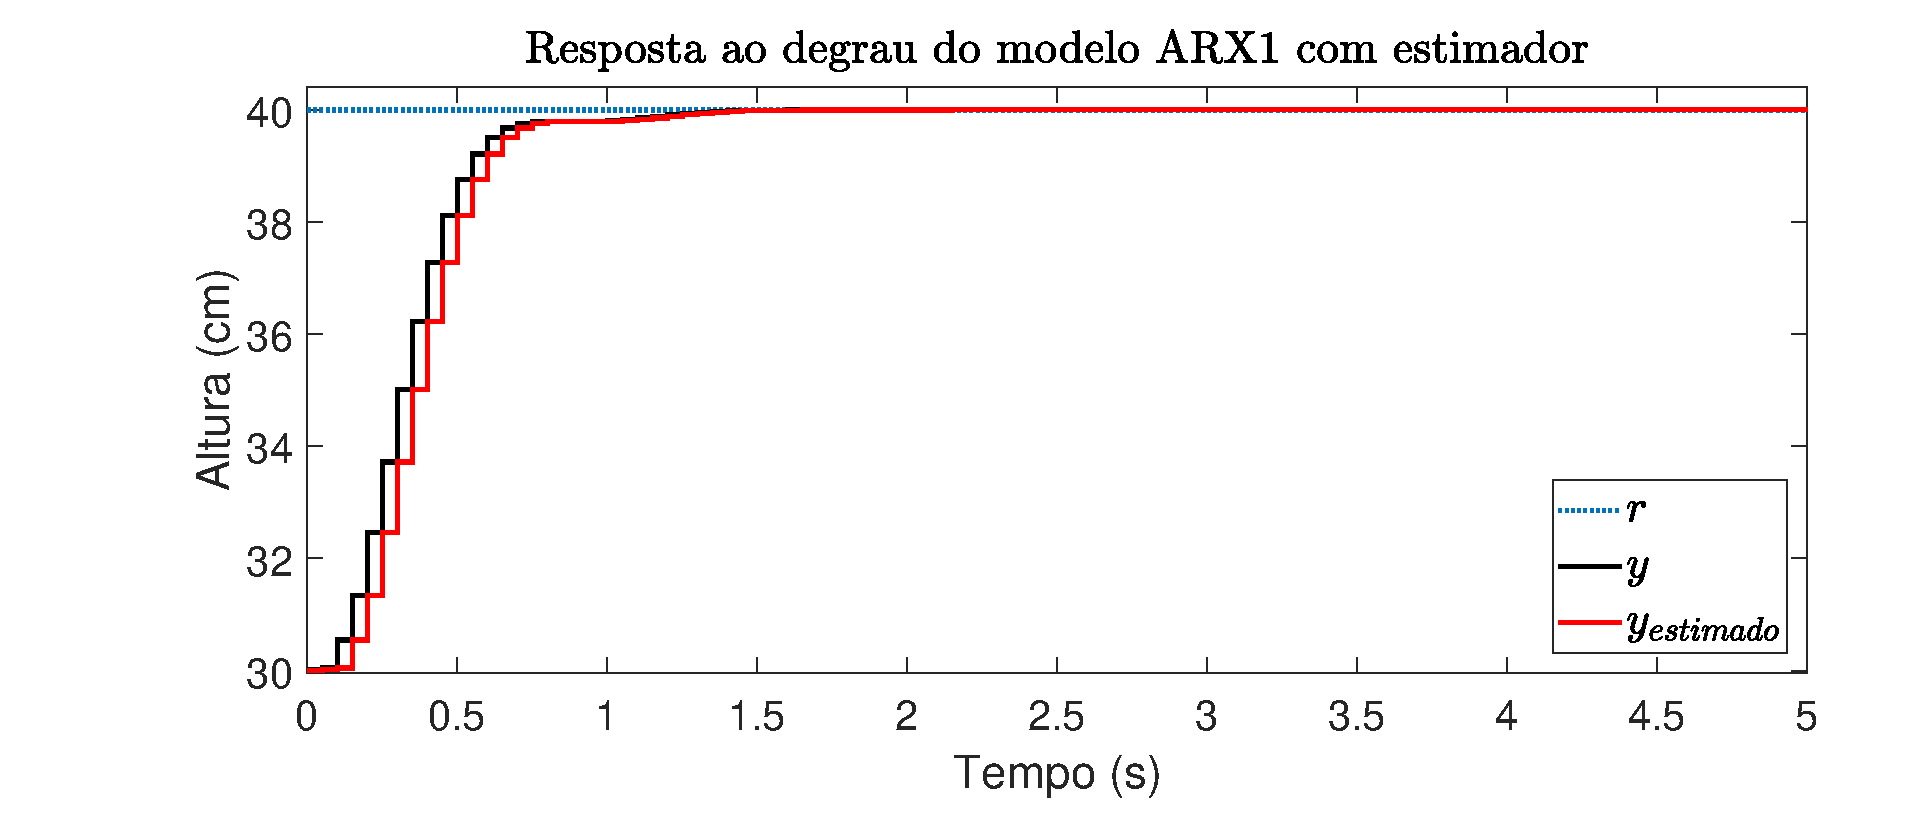
\includegraphics[width=1\linewidth]{stepestarx1}
	\caption[Resposta ao degrau do modelo $ARX1$ controlado com observador]{Resposta ao degrau do modelo $ARX1$ controlado com observador}
	\label{fig:stepestarx1}
\end{figure}

\subsection{Modelo $ARX2$}
Para o estimador do modelo $ARX2$ alocamos os polos em $z_1=0.0304 + 0.0074i$, $z_2=0.0304 - 0.0074i$, $z_3=0.0074$, $z_4=0.0072$ e $z_5=0.0069$. Obtemos o ganho do estimador $L=[22.1925,~20.4118,~ 16.9038,~16.9671,~11.1584]^T$. Nas figuras \ref{fig:estimadorarx2} e \ref{fig:stepestarx2} vemos como uma simulação do sistema se comporta.

\begin{figure}[H]
	\centering
	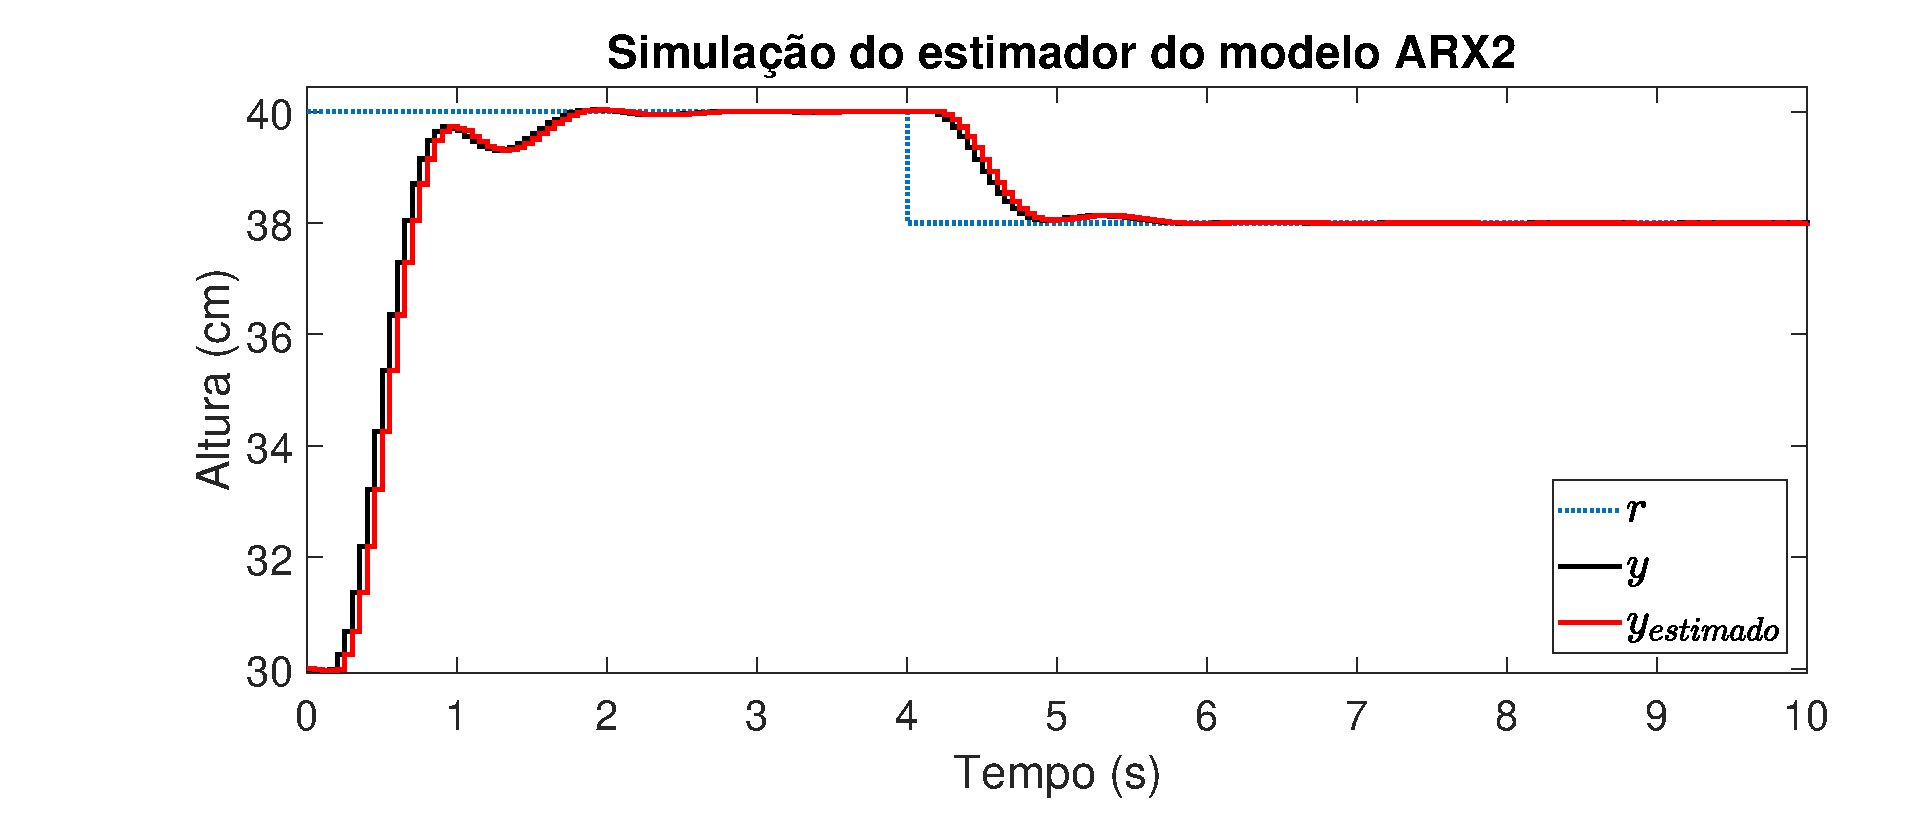
\includegraphics[width=1\linewidth]{estimadorarx2}
	\caption[Simulação do estimador do modelo $ARX2$]{Simulação do estimador do modelo $ARX2$}
	\label{fig:estimadorarx2}
\end{figure}

\begin{figure}[H]
	\centering
	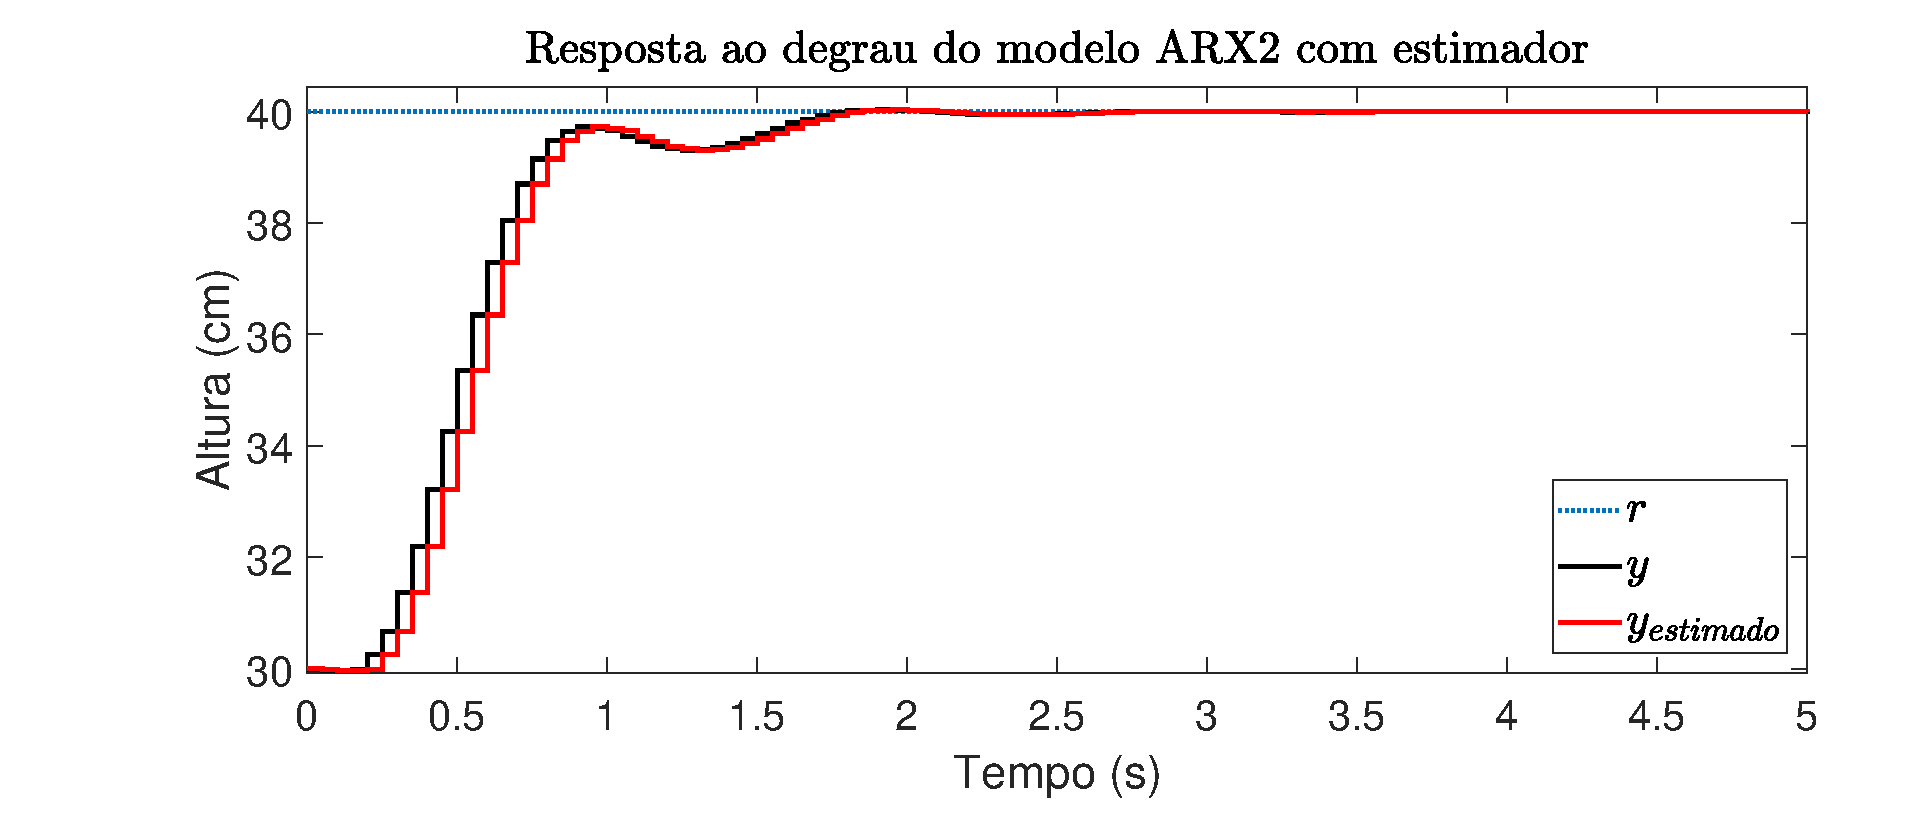
\includegraphics[width=1\linewidth]{stepestarx2}
	\caption[Resposta ao degrau do modelo $ARX2$ controlado com observador]{Resposta ao degrau do modelo $ARX2$ controlado com observador}
	\label{fig:stepestarx2}
\end{figure}

\subsection{Modelo $ARXsim$}
Para o estimador do modelo $ARX2$ alocamos os polos em $z_1=0.3383 + 0.0296i$, $z_2=0.3383 - 0.0296i$ e $z_3=0.0150$. Obtemos o ganho do estimador $L=[27.5247,~ 73.1490,~ 146.4144]^T$. Nas figuras \ref{fig:estimadorarxsim} e \ref{fig:stepestarxsim} vemos como uma simulação do sistema se comporta.

\begin{figure}[H]
	\centering
	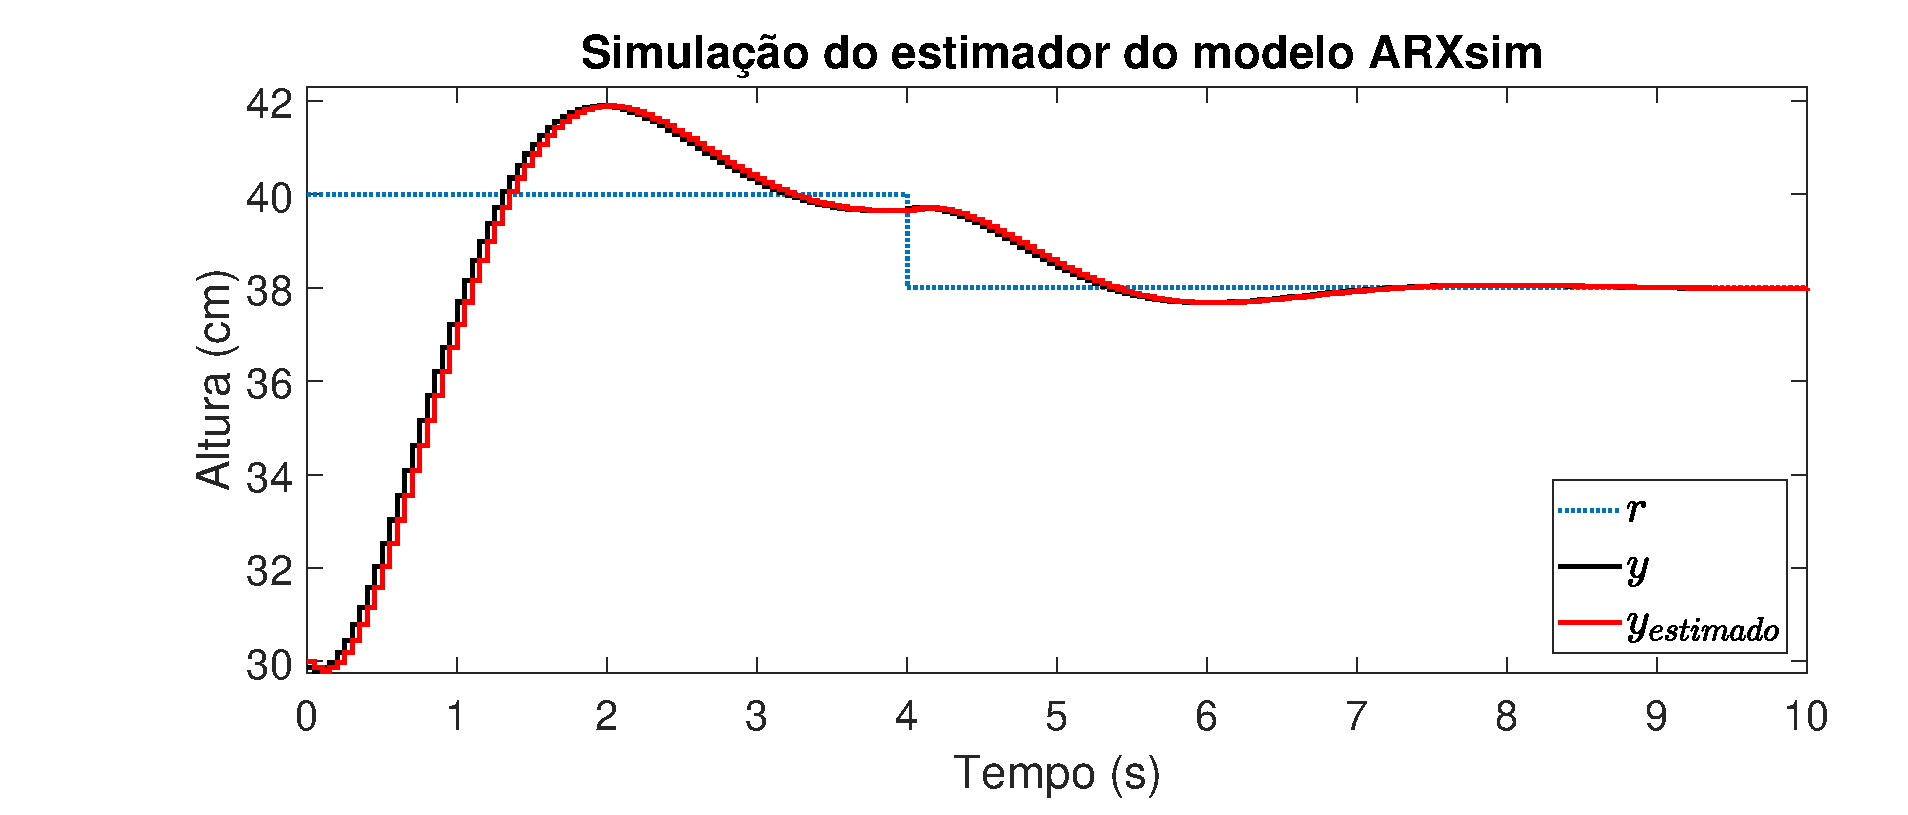
\includegraphics[width=1\linewidth]{estimadorarxsim}
	\caption[Simulação do estimador do modelo $ARXsim$]{Simulação do estimador do modelo $ARXsim$}
	\label{fig:estimadorarxsim}
\end{figure}

\begin{figure}[H]
	\centering
	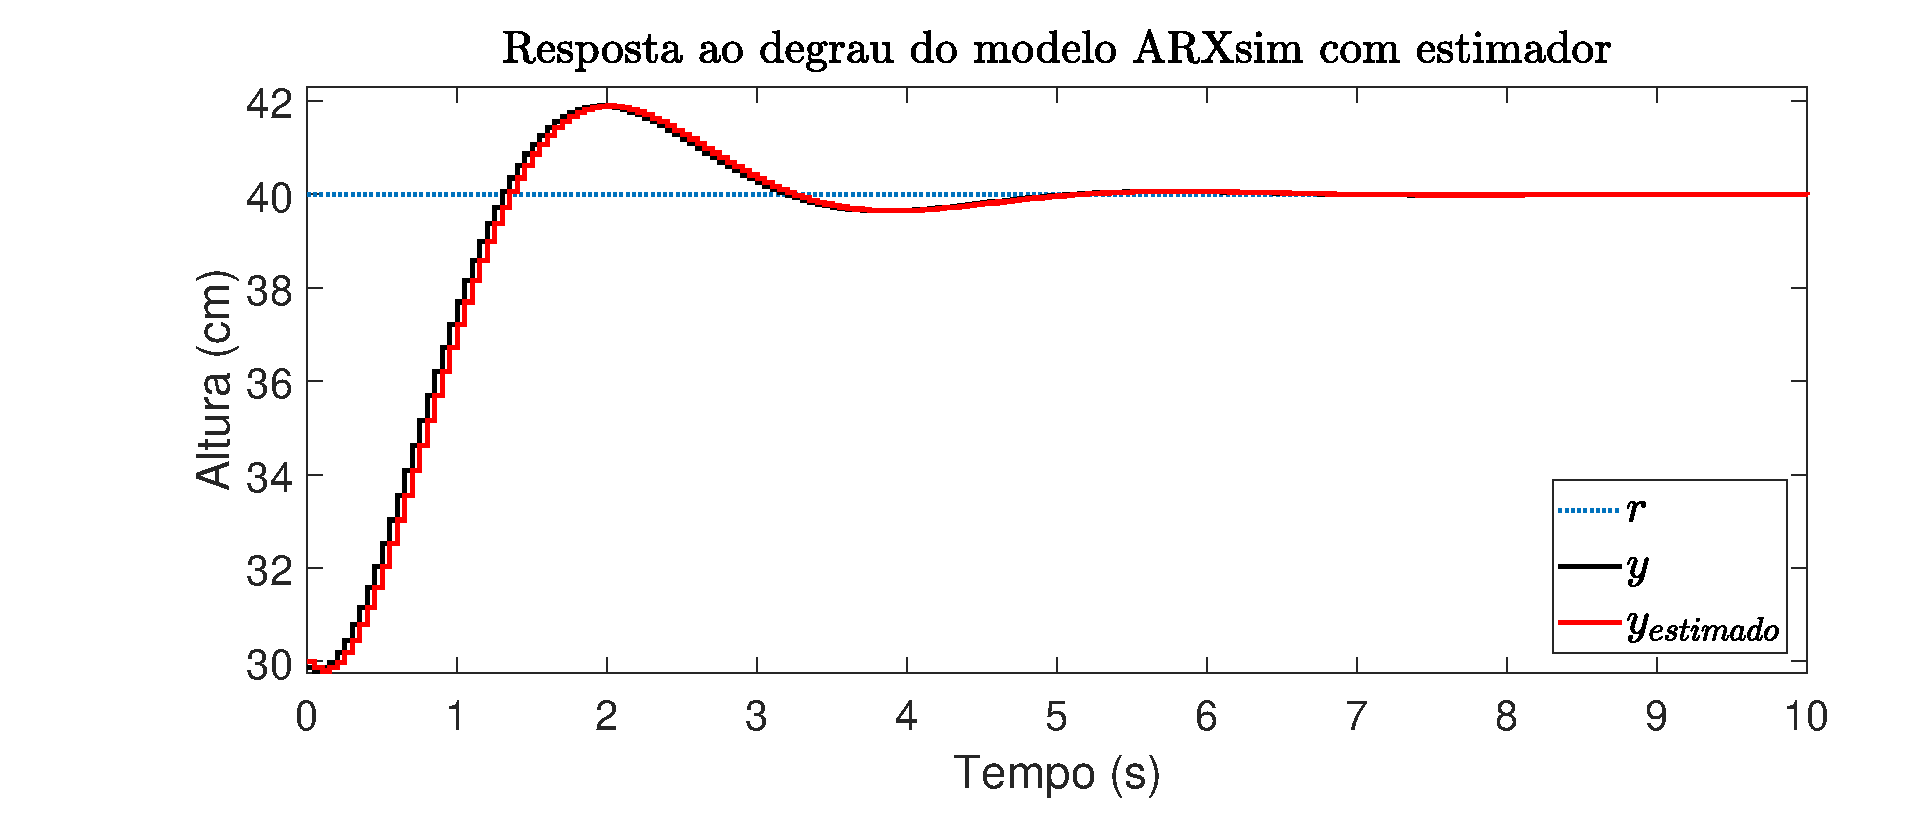
\includegraphics[width=1\linewidth]{stepestarxsim}
	\caption[Resposta ao degrau do modelo $ARXsim$ controlado com observador]{Resposta ao degrau do modelo $ARXsim$ controlado com observador}
	\label{fig:stepestarxsim}
\end{figure}














% Fim Capítulo

\chapter{Avaliação Experimental do Sistema de Controle}\label{cap6}
Após projetar os controladores faremos uma avaliação do seu funcionamento aplicando cada um no sistema real.
\section{Descrição e objetivos experimentais}
Os experimentos descritos neste capítulo tem como objetivo verificar e avaliar o funcionamento do sistema ao ser controlado pelos controladores projetados no capítulo \ref{cap5}, iremos aplicar os controladores $SUB1$, $ARX1$ e $ARX2$ no sistema real. Serão executados 4 experimentos que funcionam da seguinte forma:
\paragraph{Resposta ao Degrau Unitário} A resposta ao degrau unitário é um experimento onde o sistema recebe uma referência unitária e reage à ela. Com este experimento iremos verificar se o sistema se mantém estável ao ser controlado e se ele atende aos requisitos definidos quando o controlador foi projetado.
\paragraph{Resposta à escadaria} A resposta à escadaria é um experimento onde o sistema recebe alguns níveis de referência ao longo do tempo e medimos sua resposta para ver como reage à mudança de referência.

\paragraph{Teste de Robustez à Mudança de Parâmetros}

O teste de robustez à mudança de parâmetros serve para determinar se o controlador é capaz de reagir quando algum parâmetro é alterado. Neste experimento alteramos o peso da bola e verificamos se o sistema mantém a referência.

\paragraph{Teste de Robustez à Perturbação Externa}
  O teste de robustez à perturbação externa mostra se o sistema controlado é capaz de rejeitar perturbações externas ao sistema. Para executar este teste iremos medir a resposta do sistema enquanto obstruímos a saída de ar através dos buracos inferiores do duto do túnel de vento, efetivamente aumentando o fluxo de ar que eleva a bola.

\section{Resultados Experimentais}
Nesta seção serão apresentados os resultados dos experimentos descritos anteriormente.
\subsection{Resultados da Resposta ao degrau unitário}\label{rstep}

\subsubsection{Modelo $SUB1$}
Testamos a resposta ao degrau do modelo $SUB1$ com o sistema real e com o modelo simulado e obtemos os seguintes gráficos:

\begin{figure}[htb]
	\centering
	\begin{subfigure}[t]{0.47\textwidth}
		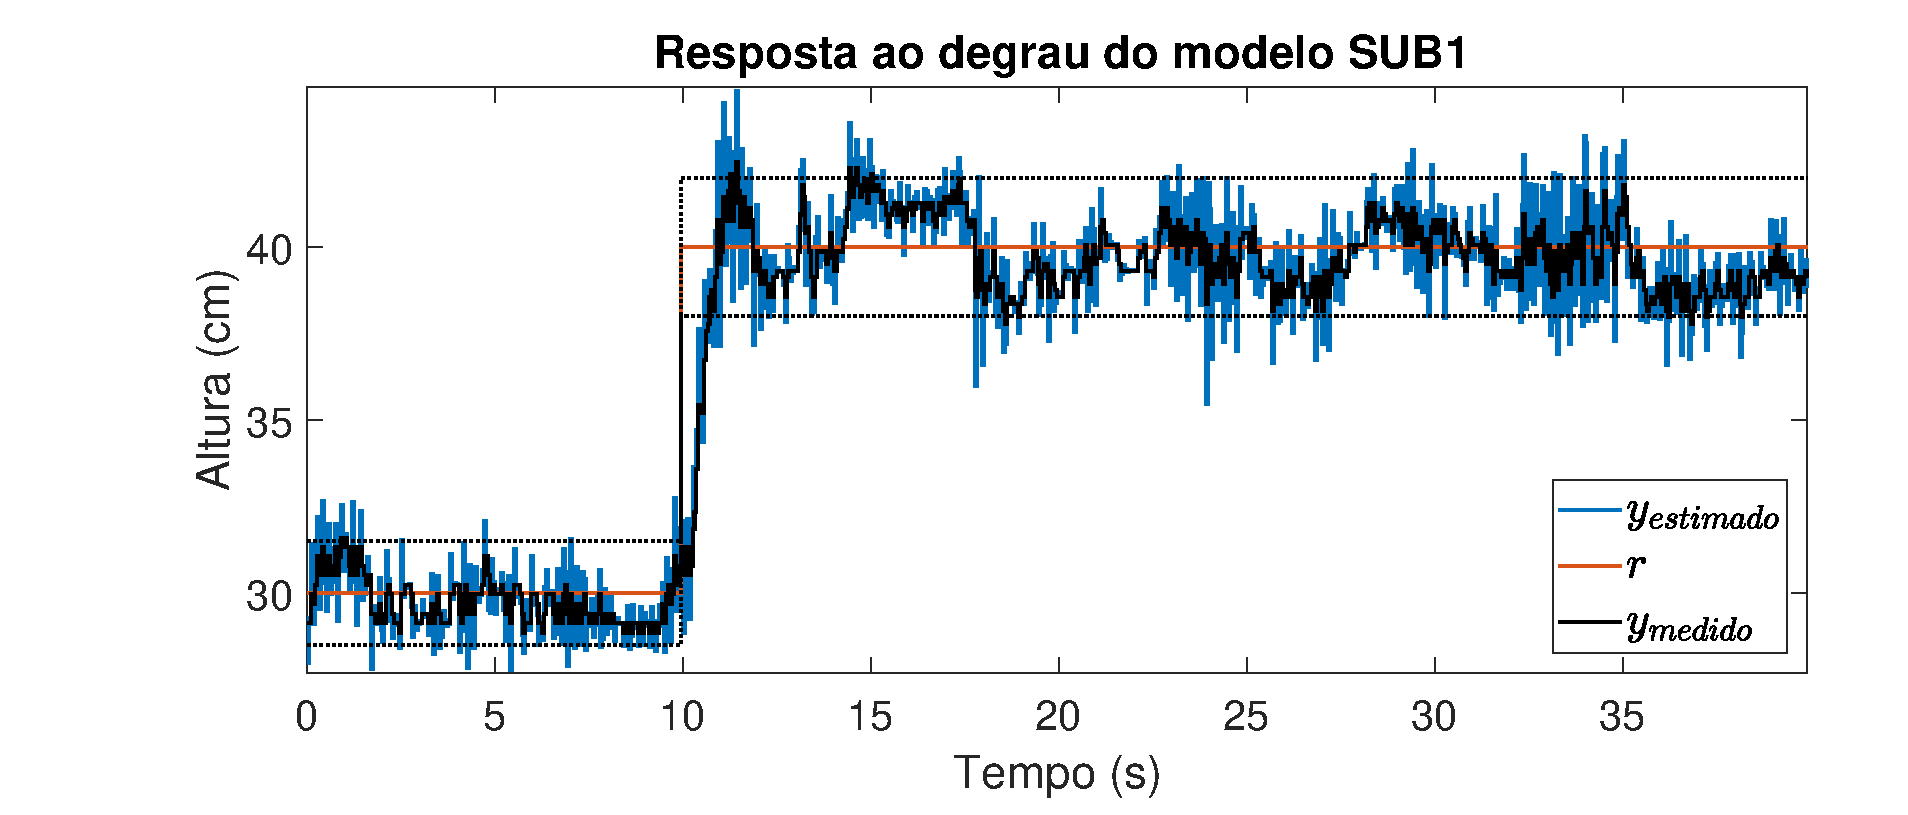
\includegraphics[width=1\linewidth]{steprsub1y}
		\subcaption[$y_{estimado}$ e $y_{medido}$ do modelo $SUB1$]{$y_{estimado}$ e $y_{medido}$ do modelo $SUB1$}
		\label{fig:steprsub1y}
	\end{subfigure}
	~ %add desired spacing between images, e. g. ~, \quad, \qquad, \hfill etc. 
	%(or a blank line to force the subfigure onto a new line)
	~
	\begin{subfigure}[t]{0.47\textwidth}
		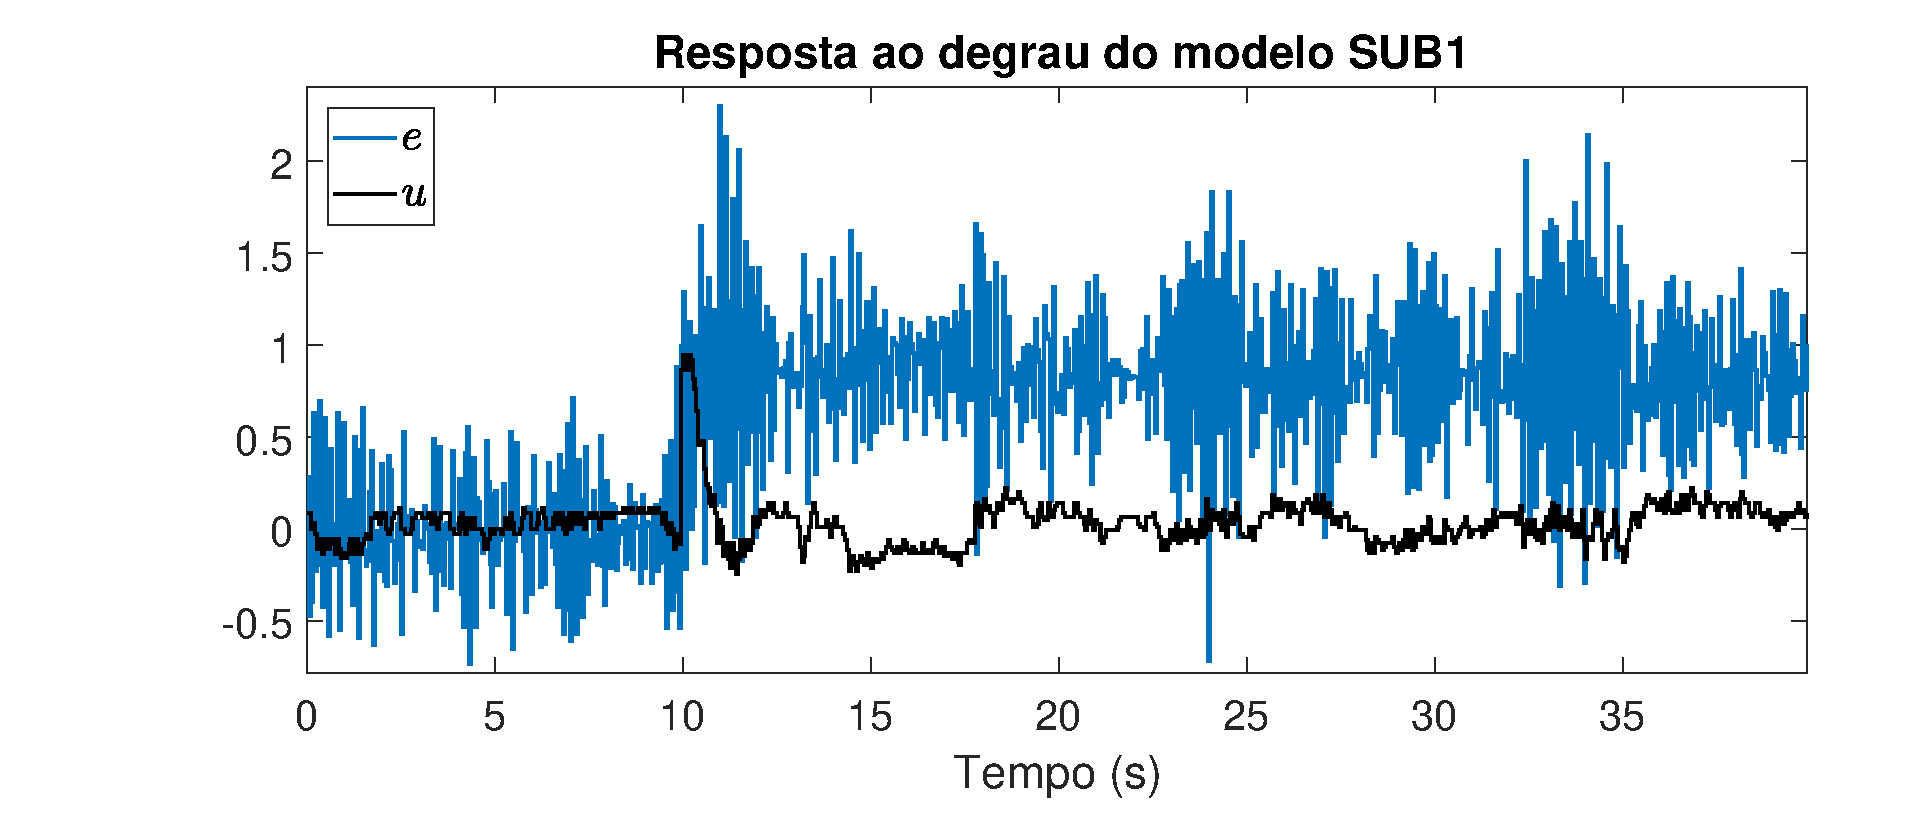
\includegraphics[width=1\linewidth]{steprsub1e}
		\subcaption[erro $e$ e sinal de controle $u$ do controlador $SUB1$]{erro $e$ e sinal de controle $u$ do controlador $SUB1$}
		\label{fig:steprsub1e}
	\end{subfigure}
	~ %add desired spacing between images, e. g. ~, \quad, \qquad, \hfill etc. 
	%(or a blank line to force the subfigure onto a new line)
	
	\caption{Resposta ao degrau do sistema usando o controlador $SUB1$}\label{fig:steprsub1}
\end{figure}

\begin{figure}[htb]
	\centering
	\begin{subfigure}[t]{0.48\textwidth}
		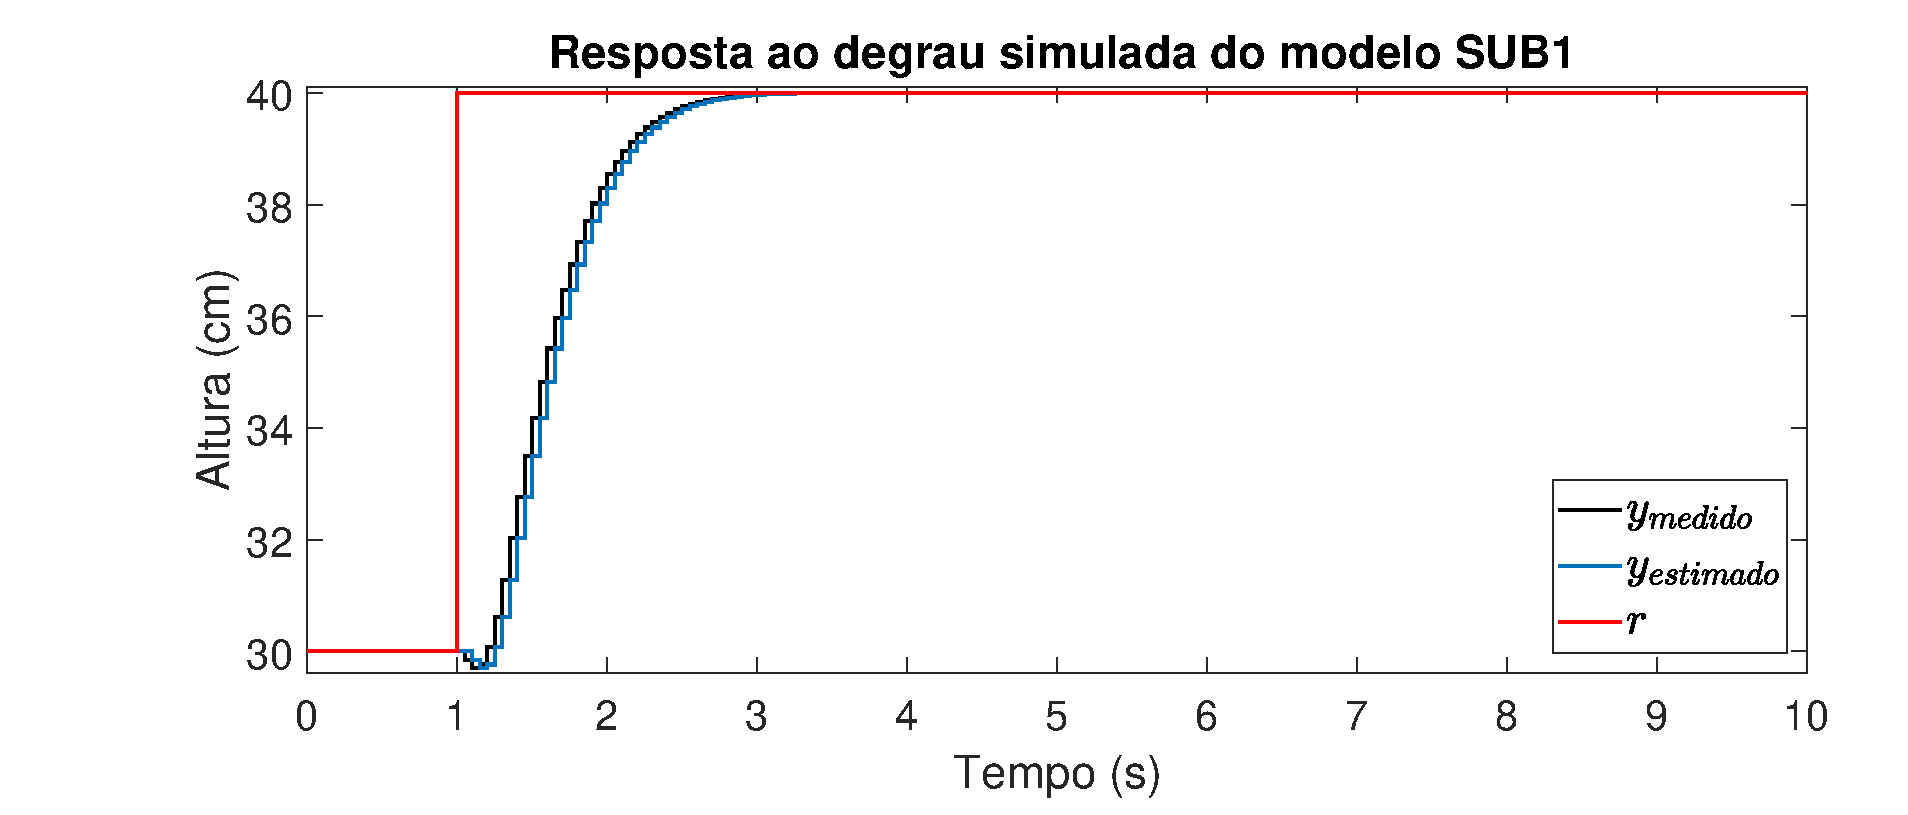
\includegraphics[width=1\linewidth]{pasta1_figuras/stepssub1y}
		\subcaption[$y_{estimado}$ e $y_{medido}$ do modelo $SUB1$]{$y_{estimado}$ e $y_{medido}$ do modelo $SUB1$}
		\label{fig:stepssub1y}
	\end{subfigure}
	~ %add desired spacing between images, e. g. ~, \quad, \qquad, \hfill etc. 
	%(or a blank line to force the subfigure onto a new line)
	\begin{subfigure}[t]{0.48\textwidth}
		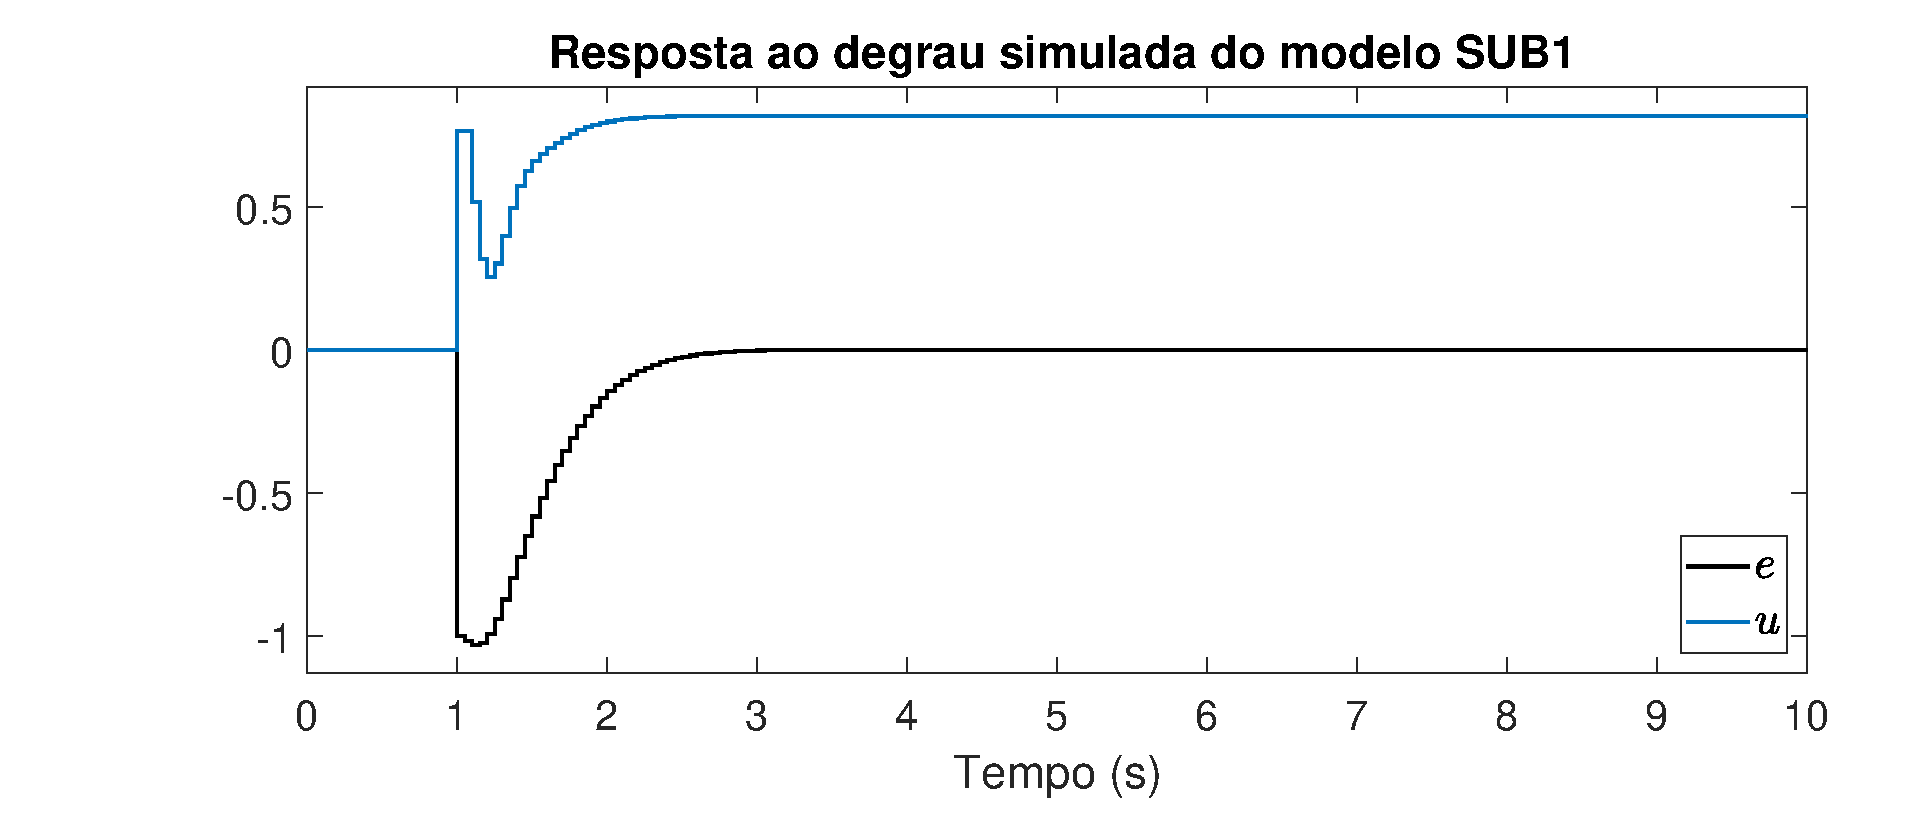
\includegraphics[width=1\linewidth]{pasta1_figuras/stepssub1e}
		\subcaption[erro $e$ e sinal de controle $u$ do controlador $SUB1$]{erro $e$ e sinal de controle $u$ do controlador $SUB1$}
		\label{fig:stepssub1e}
	\end{subfigure}
	~ %add desired spacing between images, e. g. ~, \quad, \qquad, \hfill etc. 
	%(or a blank line to force the subfigure onto a new line)
	
	\caption{Resposta ao degrau do sistema usando o controlador $SUB1$}\label{fig:stepssub1}
\end{figure}

Nos deparamos com uma grande diferença nas figuras \ref{fig:steprsub1y} e \ref{fig:stepssub1y}, a resposta simulada atende aos requisitos definidos na seção \ref{s:ctrlsub1} mas o sistema real não atende. Com um tempo de assentamento de 8 segundos muito maior que o tempo projetado. O sistema real também não atende ao requisito de máximo sobrevalor. 

\subsubsection{Modelo $ARX1$}
Testamos a resposta ao degrau do modelo $ARX1$ com o sistema real e com o modelo simulado e obtemos os seguintes gráficos:
\begin{figure}[htb]
	\centering
	\begin{subfigure}[t]{0.48\textwidth}
		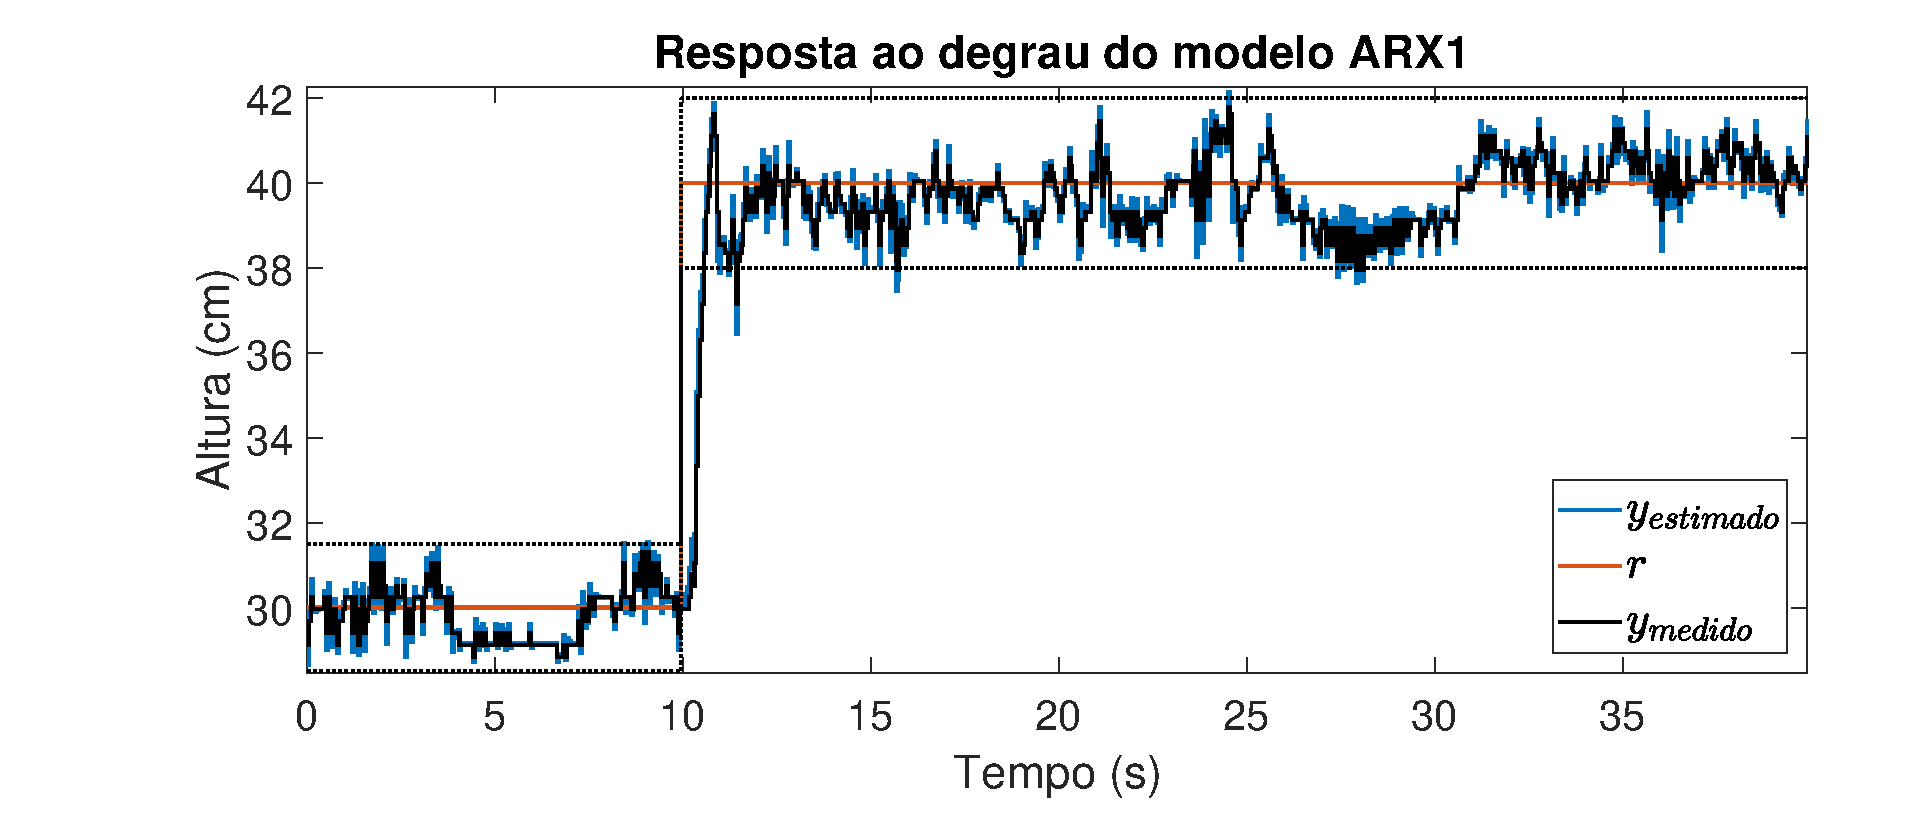
\includegraphics[width=1\linewidth]{steprarx1y}
		\caption[$y_{estimado}$ e $y_{medido}$ do modelo $ARX1$]{$y_{estimado}$ e $y_{medido}$ do modelo $ARX1$}
		\label{fig:steprarx1y}
	\end{subfigure}
	~ %add desired spacing between images, e. g. ~, \quad, \qquad, \hfill etc. 
	%(or a blank line to force the subfigure onto a new line)
	\begin{subfigure}[t]{0.48\textwidth}
		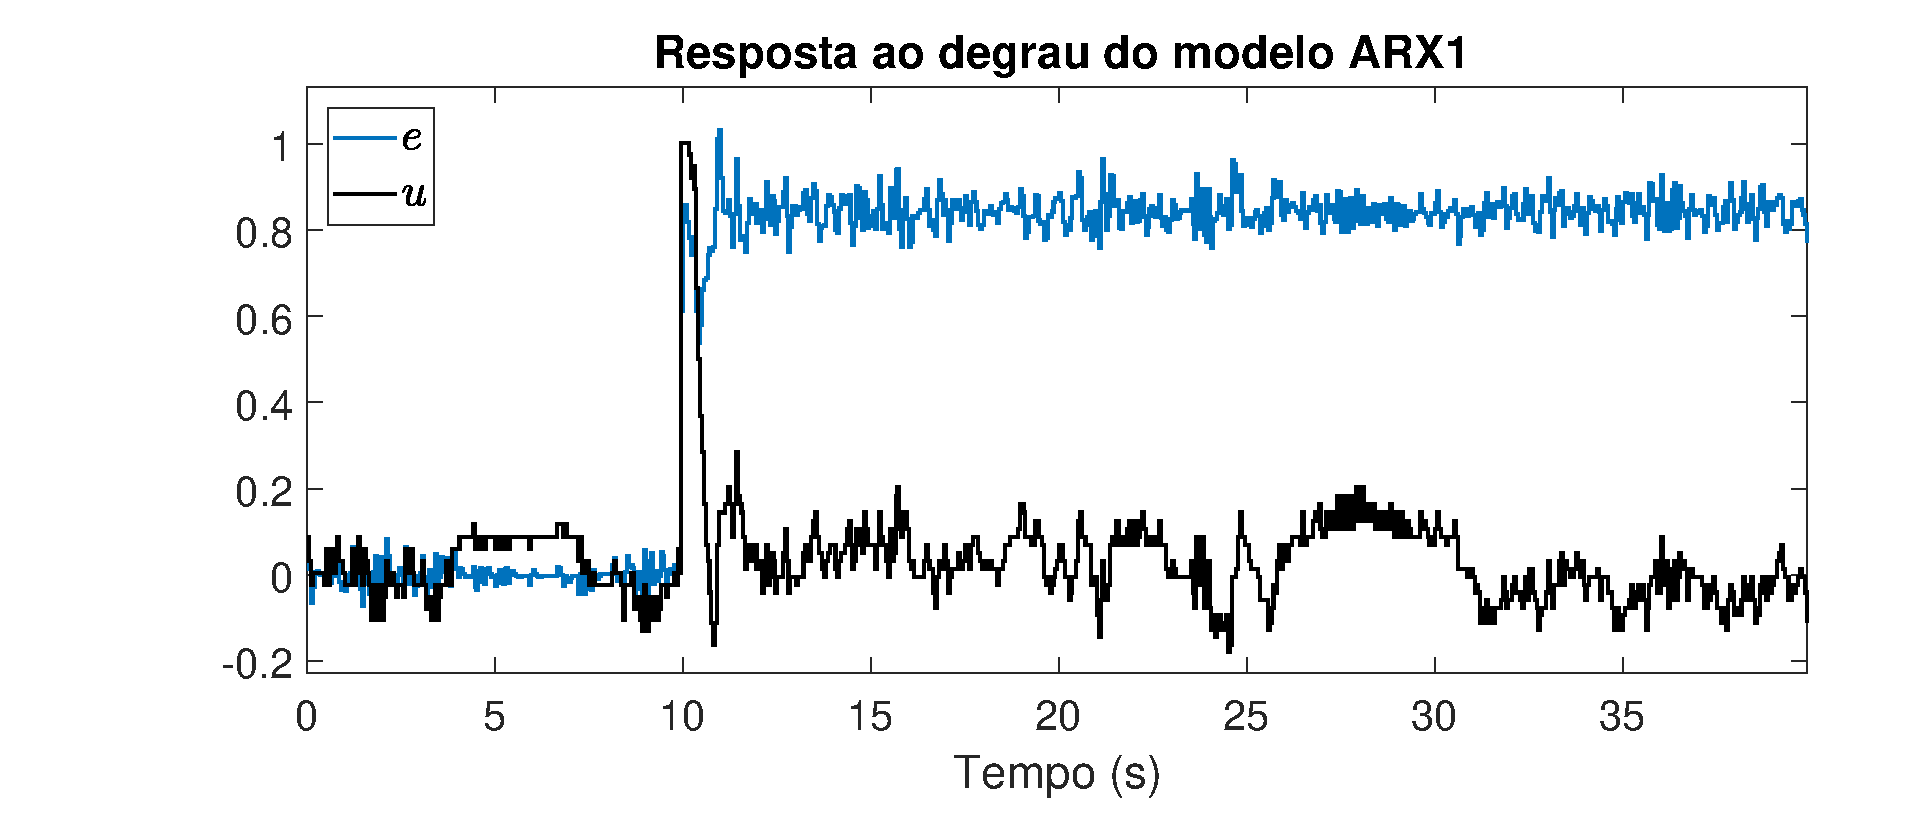
\includegraphics[width=1\linewidth]{steprarx1e}
		\caption[erro $e$ e sinal de controle $u$ do controlador $ARX1$]{erro $e$ e sinal de controle $u$ do controlador $ARX1$}
		\label{fig:steprarx1e}
	\end{subfigure}
	~ %add desired spacing between images, e. g. ~, \quad, \qquad, \hfill etc. 
	%(or a blank line to force the subfigure onto a new line)
	
	\caption{Resposta à perturbação externa do sistema com o controlador do modelo $ARX1$}\label{fig:steprarx1}
\end{figure}



Vemos na figuras \ref{fig:steprarx1y}


\subsubsection{Modelo $ARX2$}
Testamos a resposta ao degrau do modelo $ARX2$ com o sistema real e com o modelo simulado e obtemos os seguintes gráficos:
\begin{figure}[htb]
	\centering
	\begin{subfigure}[t]{0.48\textwidth}
		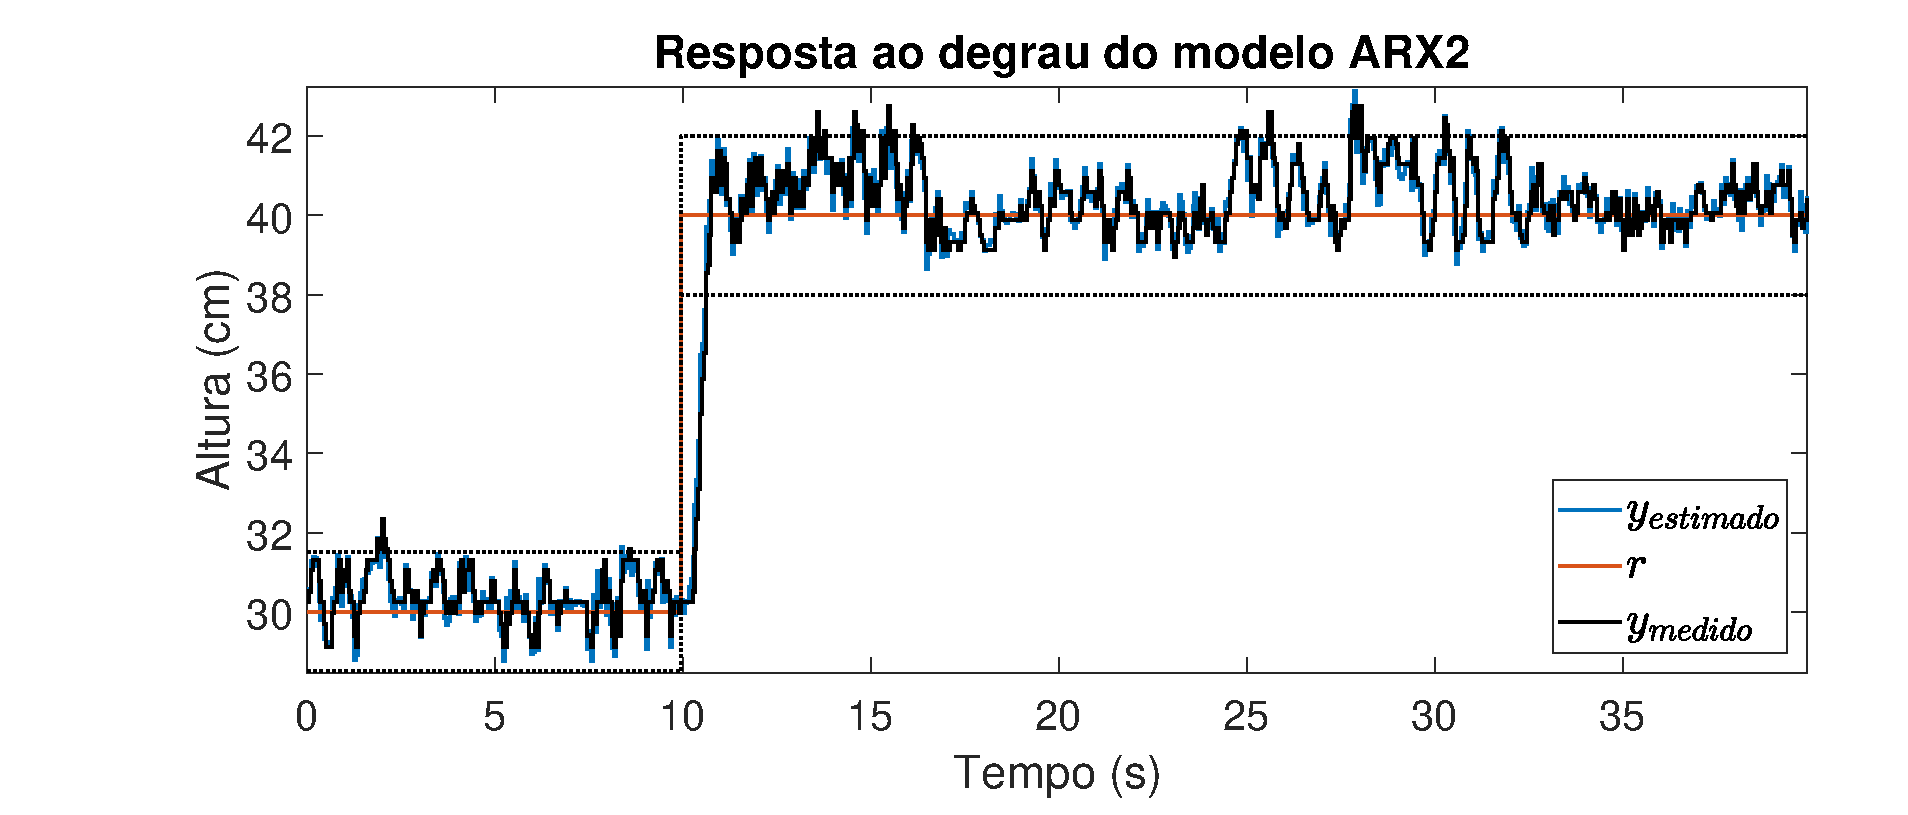
\includegraphics[width=1\linewidth]{steprarx2y}
		\caption[$y_{estimado}$ e $y_{medido}$ do modelo $ARX2$]{$y_{estimado}$ e $y_{medido}$ do modelo $ARX2$}
		\label{fig:steprarx2y}
	\end{subfigure}
	~ %add desired spacing between images, e. g. ~, \quad, \qquad, \hfill etc. 
	%(or a blank line to force the subfigure onto a new line)
	\begin{subfigure}[t]{0.48\textwidth}
		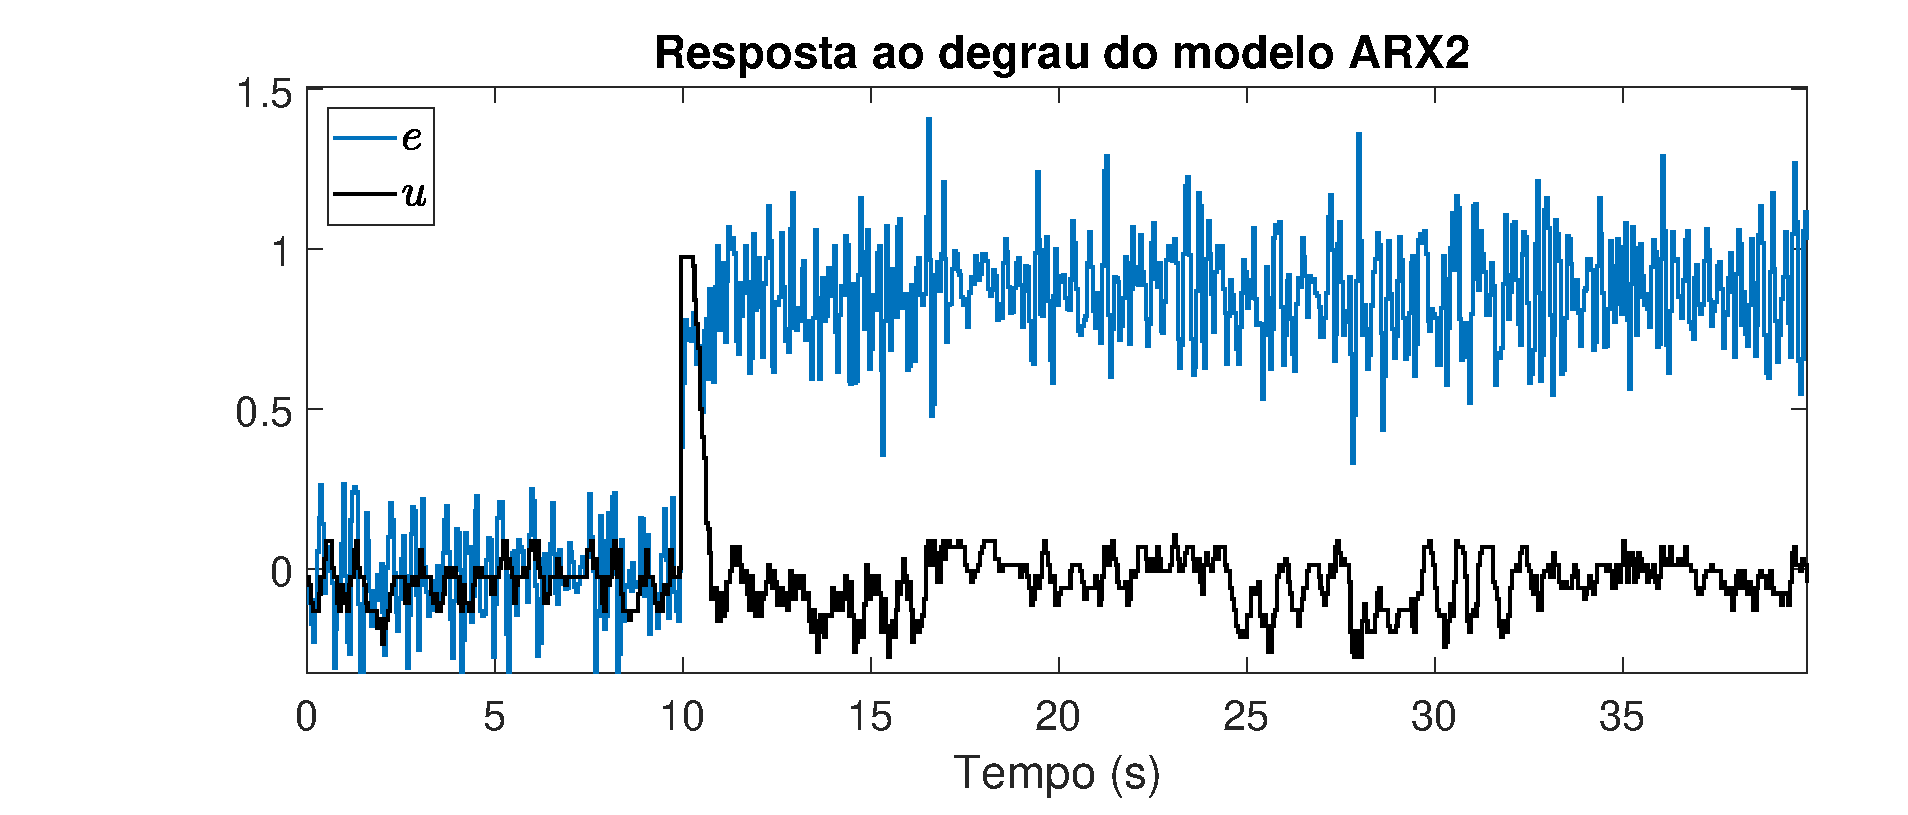
\includegraphics[width=1\linewidth]{steprarx2e}
		\caption[erro $e$ e sinal de controle $u$ do controlador $ARX2$]{erro $e$ e sinal de controle $u$ do controlador $ARX2$}
		\label{fig:steprarx2e}
	\end{subfigure}
	~ %add desired spacing between images, e. g. ~, \quad, \qquad, \hfill etc. 
	%(or a blank line to force the subfigure onto a new line)
	
	\caption{Resposta à perturbação externa do sistema com o controlador do modelo $ARX2$}\label{fig:steprarx2}
\end{figure}
Vemos na figuras \ref{fig:steprarx2y}

\subsection{Resultados da Resposta à escadaria}\label{rstair}

\subsubsection{Modelo $SUB1$}
Testamos a resposta à escadaria do modelo $SUB1$ com o sistema real e com o modelo simulado e obtemos os seguintes gráficos:
\begin{figure}[htb]
	\centering
	\begin{subfigure}[t]{0.48\textwidth}
		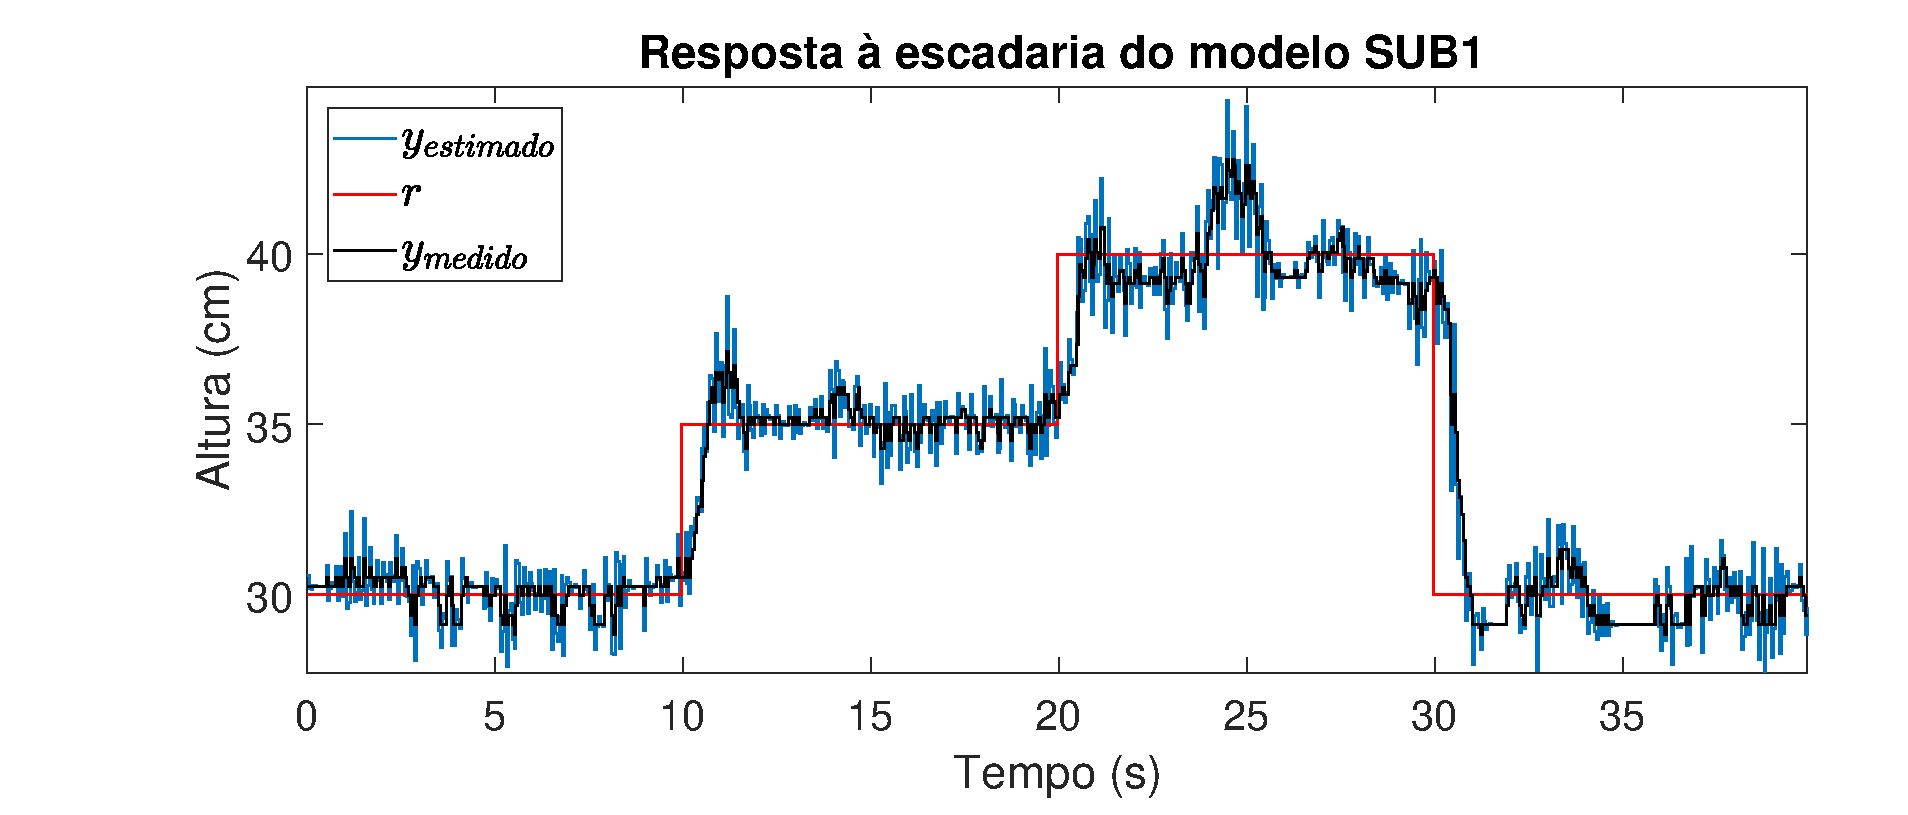
\includegraphics[width=1\linewidth]{stairrsub1y}
		\caption[$y_{estimado}$ e $y_{medido}$ do modelo $SUB1$]{$y_{estimado}$ e $y_{medido}$ do modelo $SUB1$}
		\label{fig:stairrsub1y}
	\end{subfigure}
	~ %add desired spacing between images, e. g. ~, \quad, \qquad, \hfill etc. 
	%(or a blank line to force the subfigure onto a new line)
	\begin{subfigure}[t]{0.48\textwidth}
		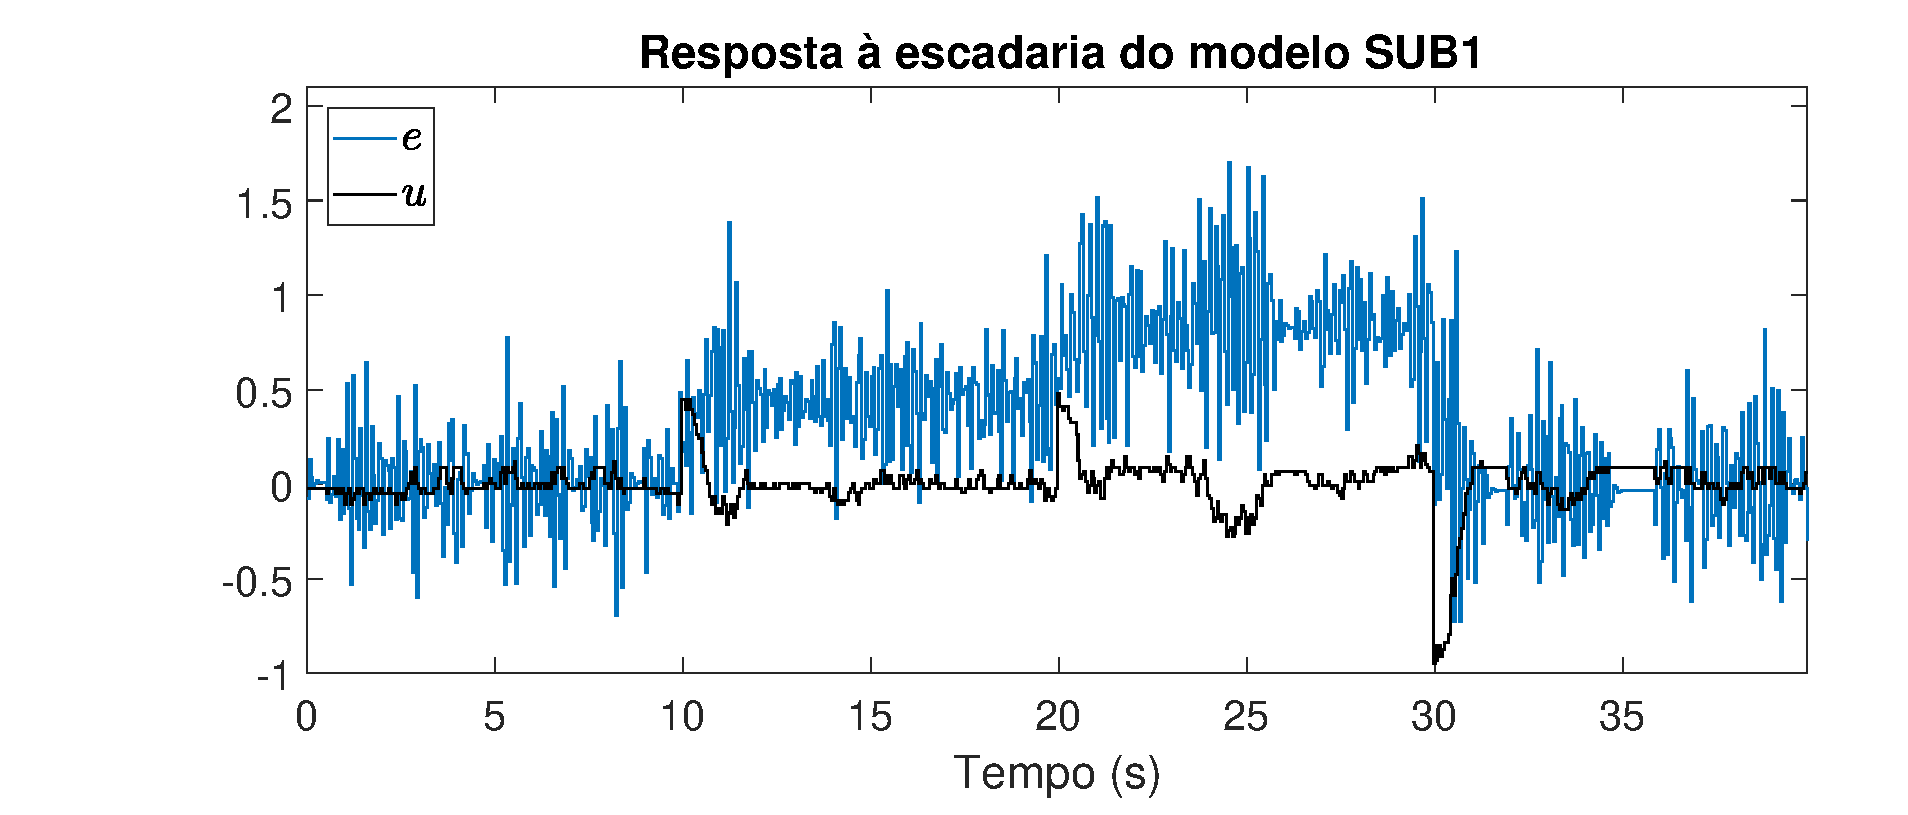
\includegraphics[width=1\linewidth]{stairrsub1e}
		\caption[erro $e$ e sinal de controle $u$ do controlador $SUB1$]{erro $e$ e sinal de controle $u$ do controlador $SUB1$}
		\label{fig:stairrsub1e}
	\end{subfigure}
	~ %add desired spacing between images, e. g. ~, \quad, \qquad, \hfill etc. 
	%(or a blank line to force the subfigure onto a new line)
	
	\caption{Resposta à perturbação externa do sistema com o controlador do modelo $SUB1$}\label{fig:stairrsub1}
\end{figure}

Vemos na figuras \ref{fig:stairsub1y}

\subsubsection{Modelo $ARX1$}
Testamos a resposta à escadaria do modelo $ARX1$ com o sistema real e com o modelo simulado e obtemos os seguintes gráficos:

\begin{figure}[htb]
	\centering
	\begin{subfigure}[t]{0.48\textwidth}
		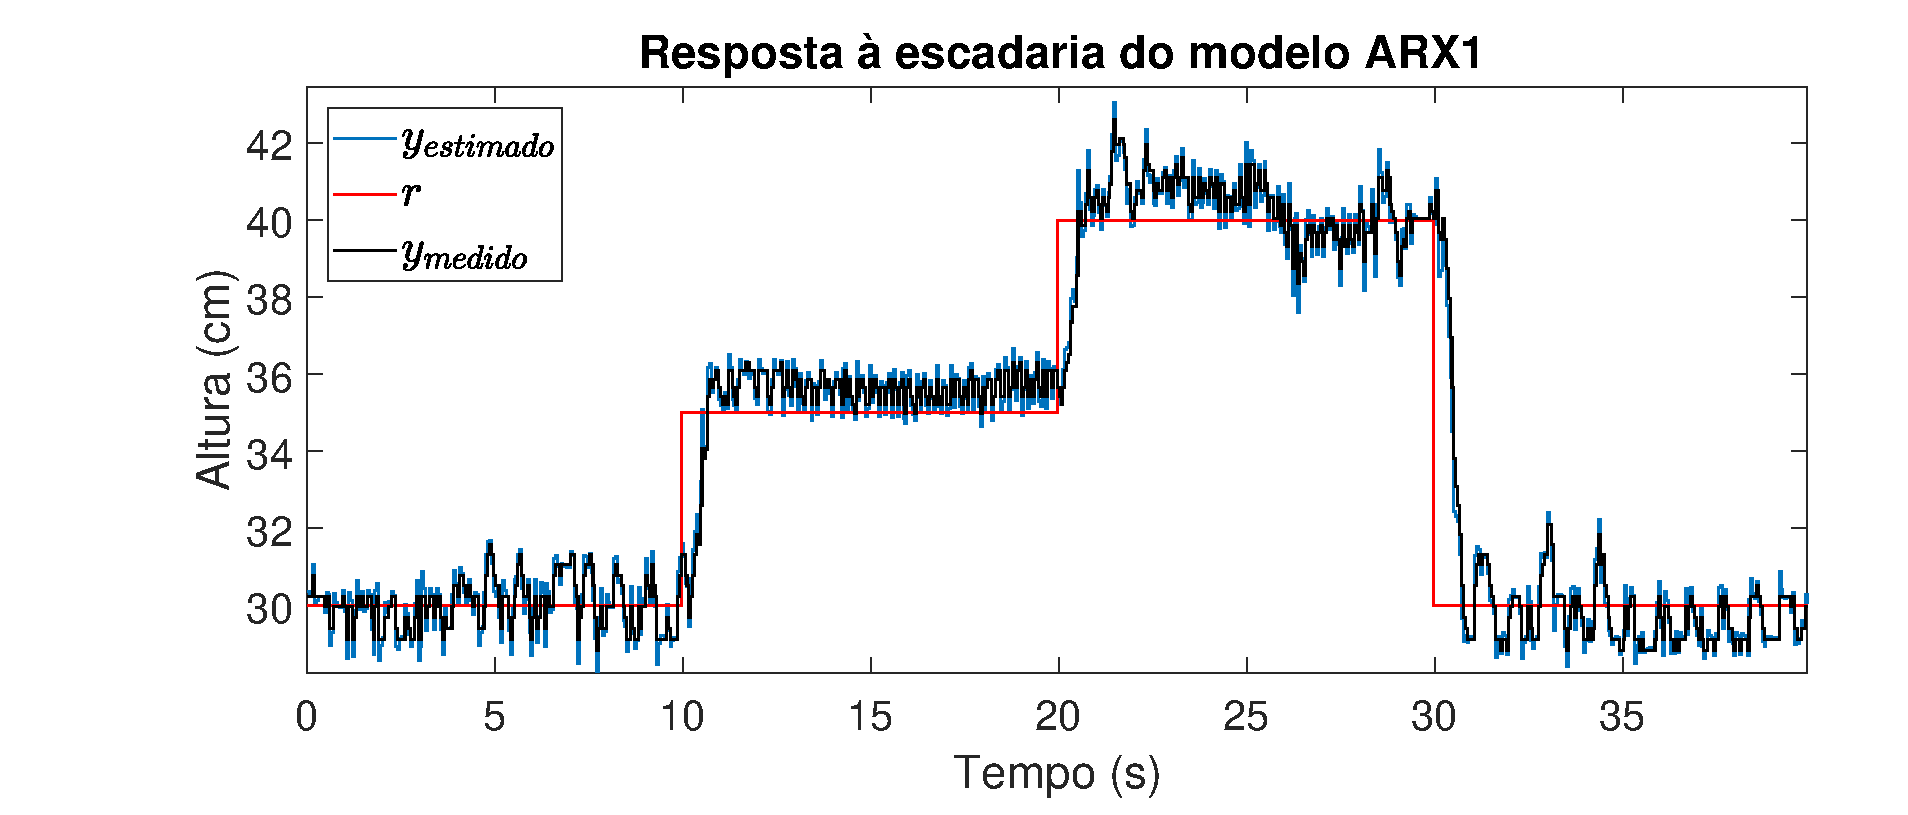
\includegraphics[width=1\linewidth]{stairrarx1y}
		\caption[$y_{estimado}$ e $y_{medido}$ do modelo $ARX1$]{$y_{estimado}$ e $y_{medido}$ do modelo $ARX1$}
		\label{fig:stairrarx1y}
	\end{subfigure}
	~ %add desired spacing between images, e. g. ~, \quad, \qquad, \hfill etc. 
	%(or a blank line to force the subfigure onto a new line)
	\begin{subfigure}[t]{0.48\textwidth}
		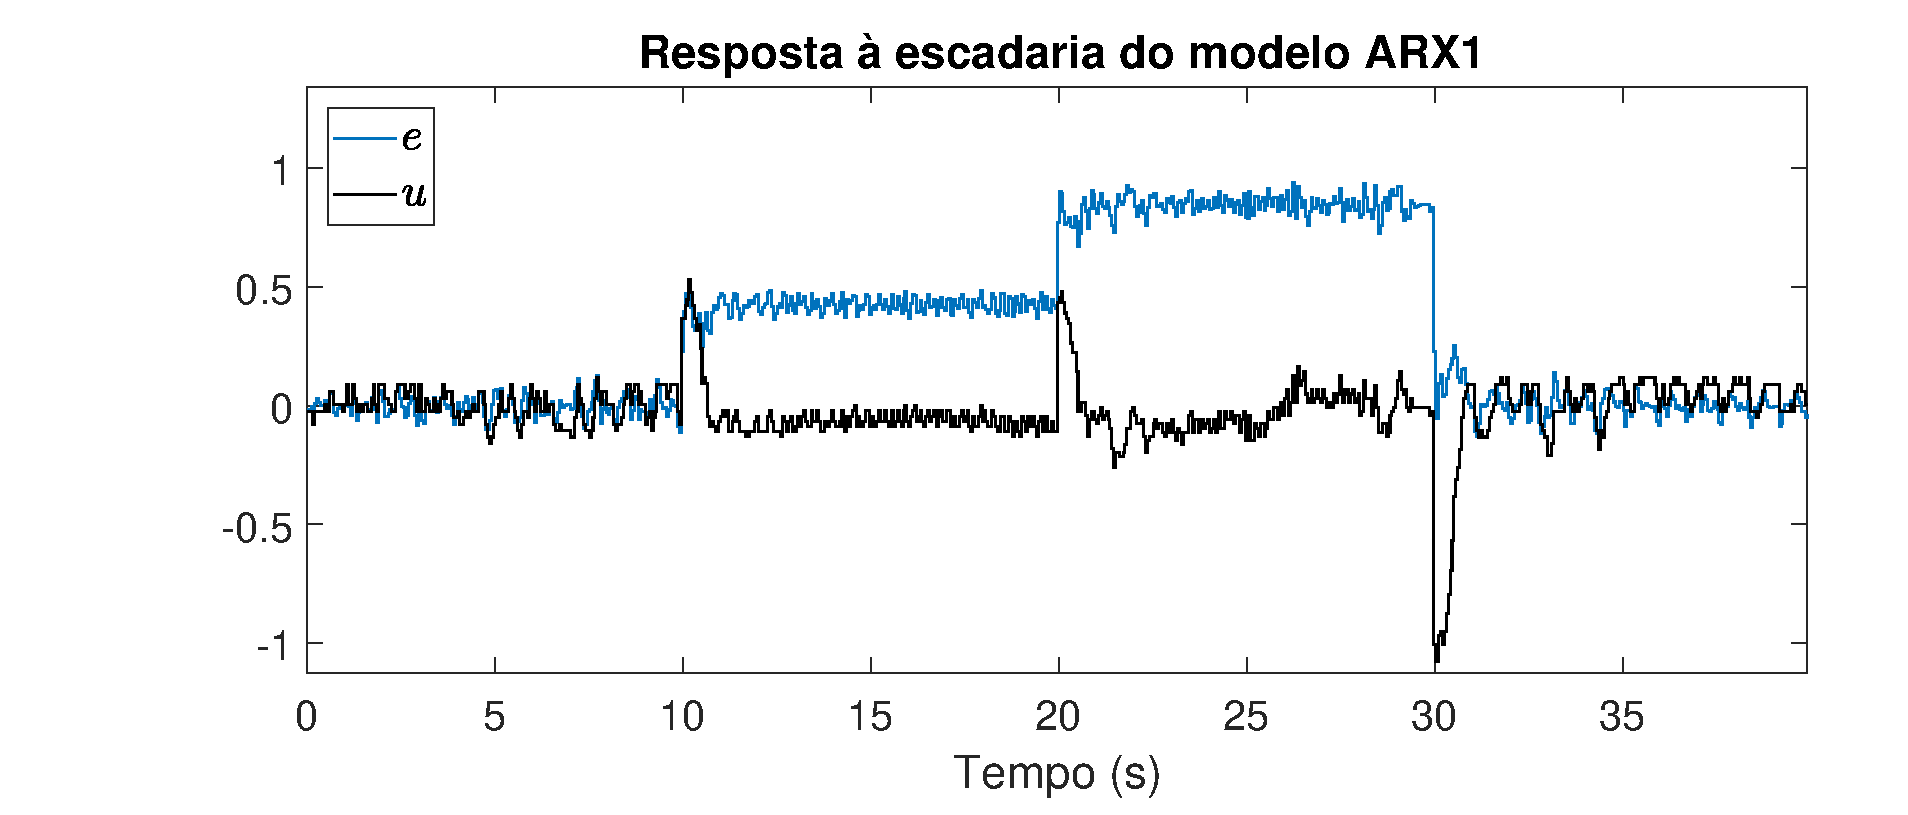
\includegraphics[width=1\linewidth]{stairrarx1e}
		\caption[erro $e$ e sinal de controle $u$ do controlador $ARX1$]{erro $e$ e sinal de controle $u$ do controlador $ARX1$}
		\label{fig:stairrarx1e}
	\end{subfigure}
	~ %add desired spacing between images, e. g. ~, \quad, \qquad, \hfill etc. 
	%(or a blank line to force the subfigure onto a new line)
	
	\caption{Resposta à perturbação externa do sistema com o controlador do modelo $ARX1$}\label{fig:stairrarx1}
\end{figure}

Vemos na figuras \ref{fig:stairarx1y}

\subsubsection{Modelo $ARX2$}
Testamos a resposta à escadaria do modelo $ARX2$ com o sistema real e com o modelo simulado e obtemos os seguintes gráficos:

\begin{figure}[htb]
	\centering
	\begin{subfigure}[t]{0.48\textwidth}
		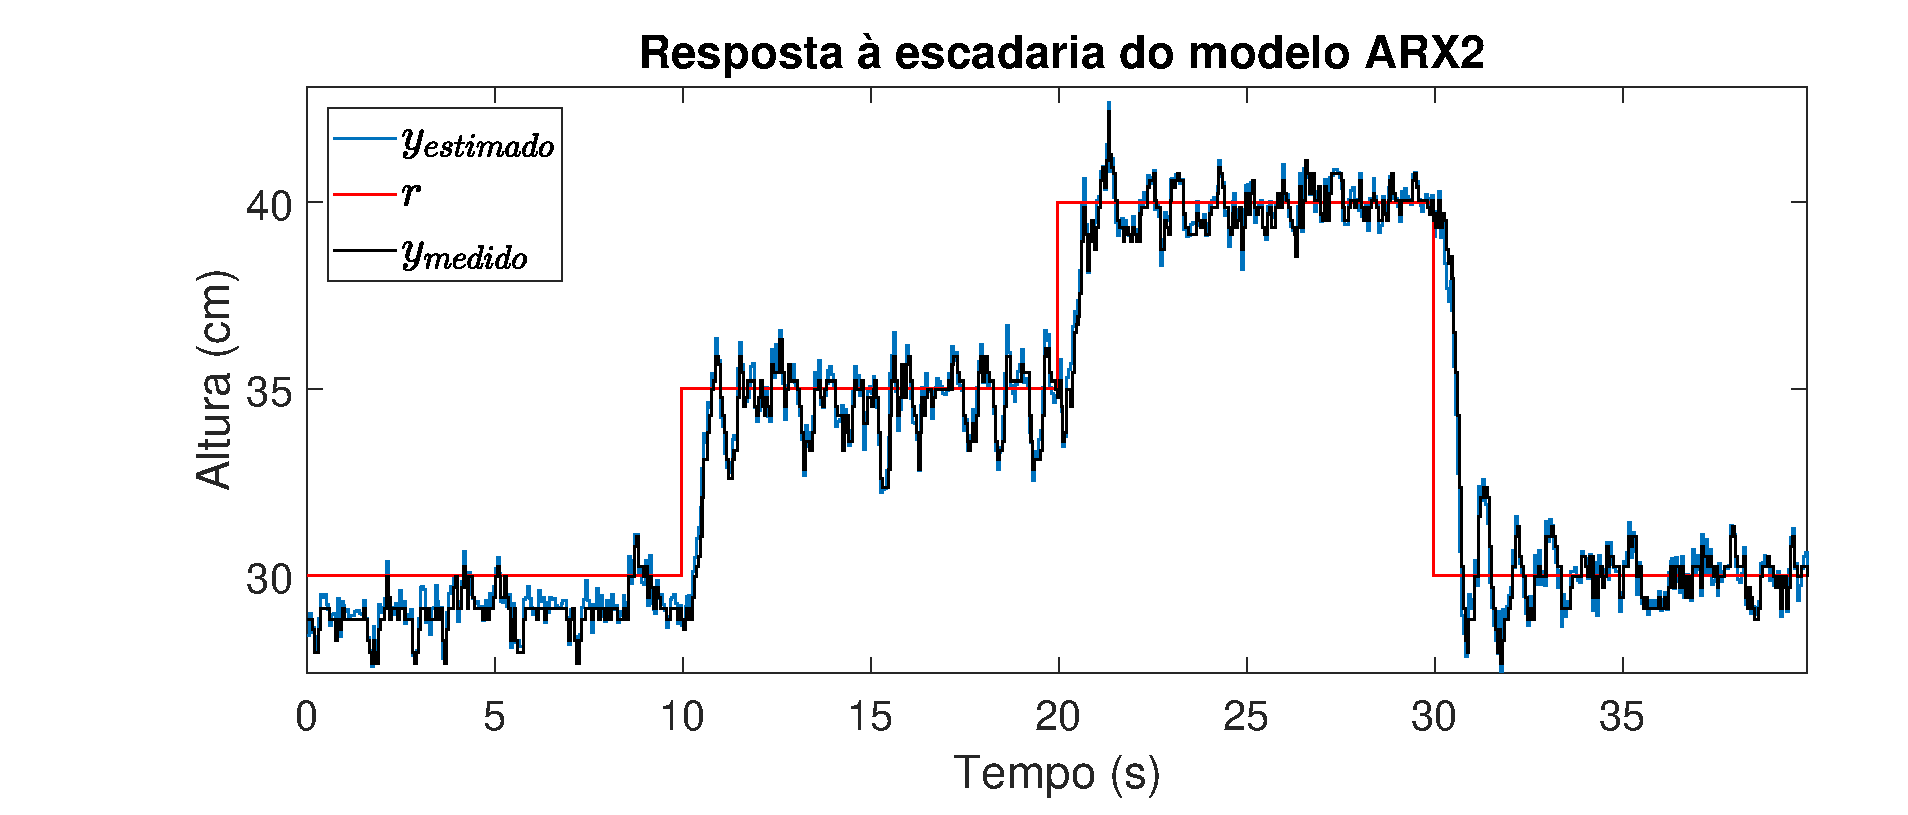
\includegraphics[width=1\linewidth]{stairrarx2y}
		\caption[$y_{estimado}$ e $y_{medido}$ do modelo $ARX2$]{$y_{estimado}$ e $y_{medido}$ do modelo $ARX2$}
		\label{fig:stairrarx2y}
	\end{subfigure}
	~ %add desired spacing between images, e. g. ~, \quad, \qquad, \hfill etc. 
	%(or a blank line to force the subfigure onto a new line)
	\begin{subfigure}[t]{0.48\textwidth}
		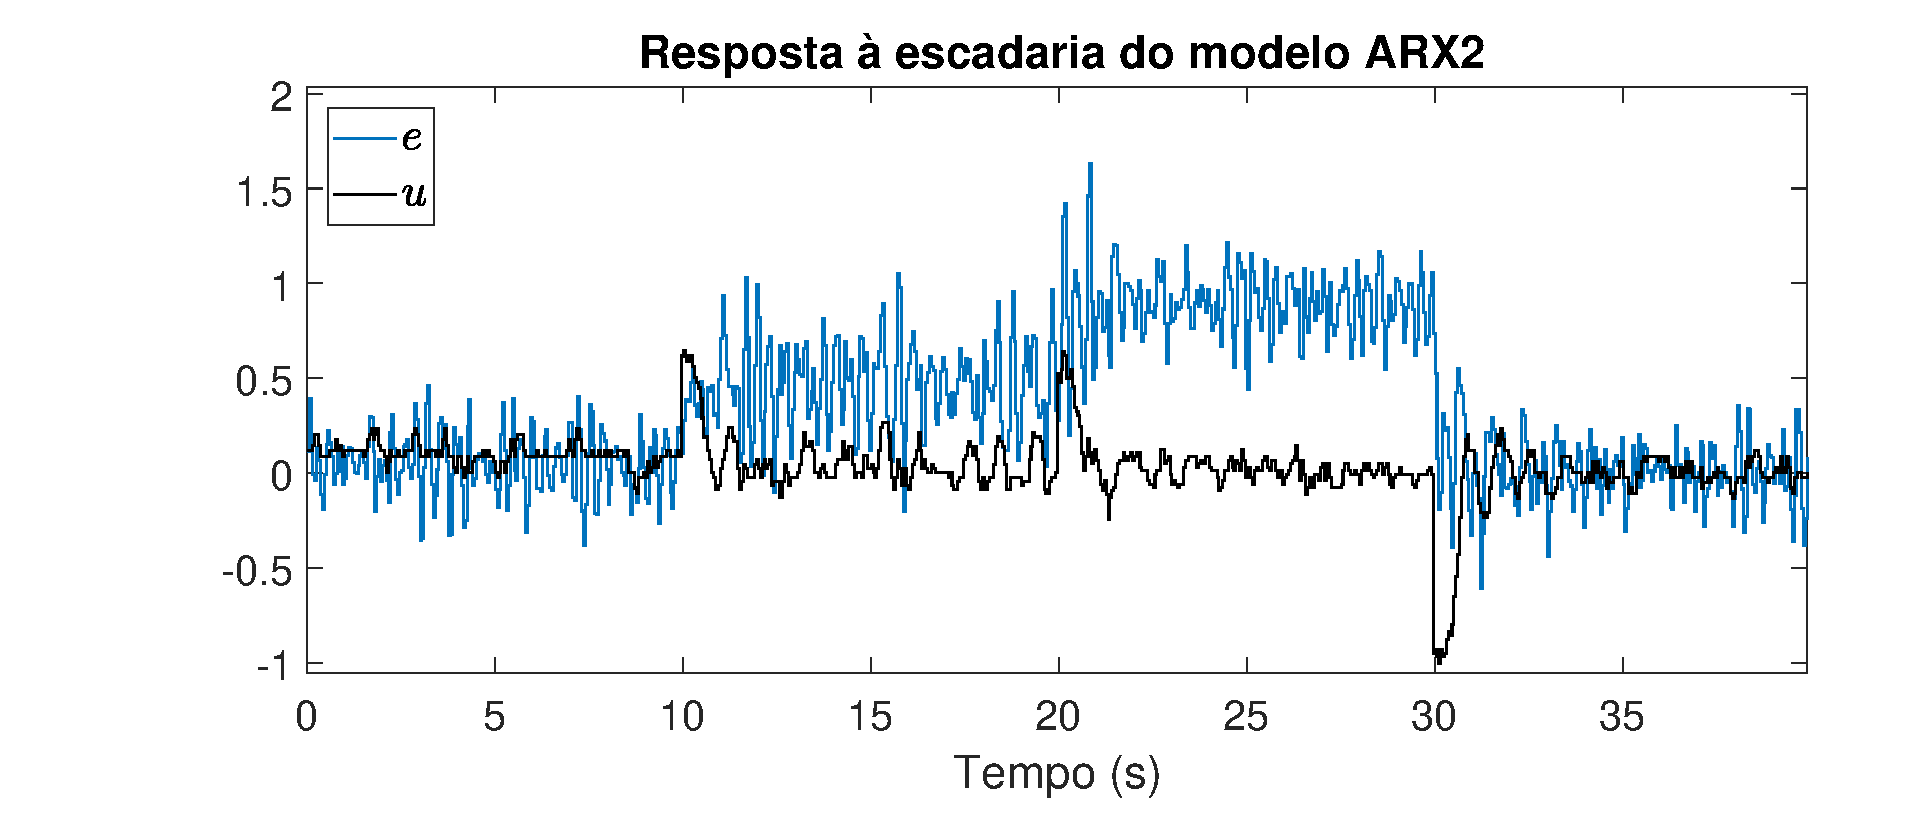
\includegraphics[width=1\linewidth]{stairrarx2e}
		\caption[erro $e$ e sinal de controle $u$ do controlador $ARX2$]{erro $e$ e sinal de controle $u$ do controlador $ARX2$}
		\label{fig:stairrarx2e}
	\end{subfigure}
	~ %add desired spacing between images, e. g. ~, \quad, \qquad, \hfill etc. 
	%(or a blank line to force the subfigure onto a new line)
	
	\caption{Resposta à perturbação externa do sistema com o controlador do modelo $ARX2$}\label{fig:stairrarx2}
\end{figure}

Vemos na figuras \ref{fig:stairarx2y}

\subsubsection{Erro do Estimador} \label{erroest}

\begin{figure}[htb]
	\centering
	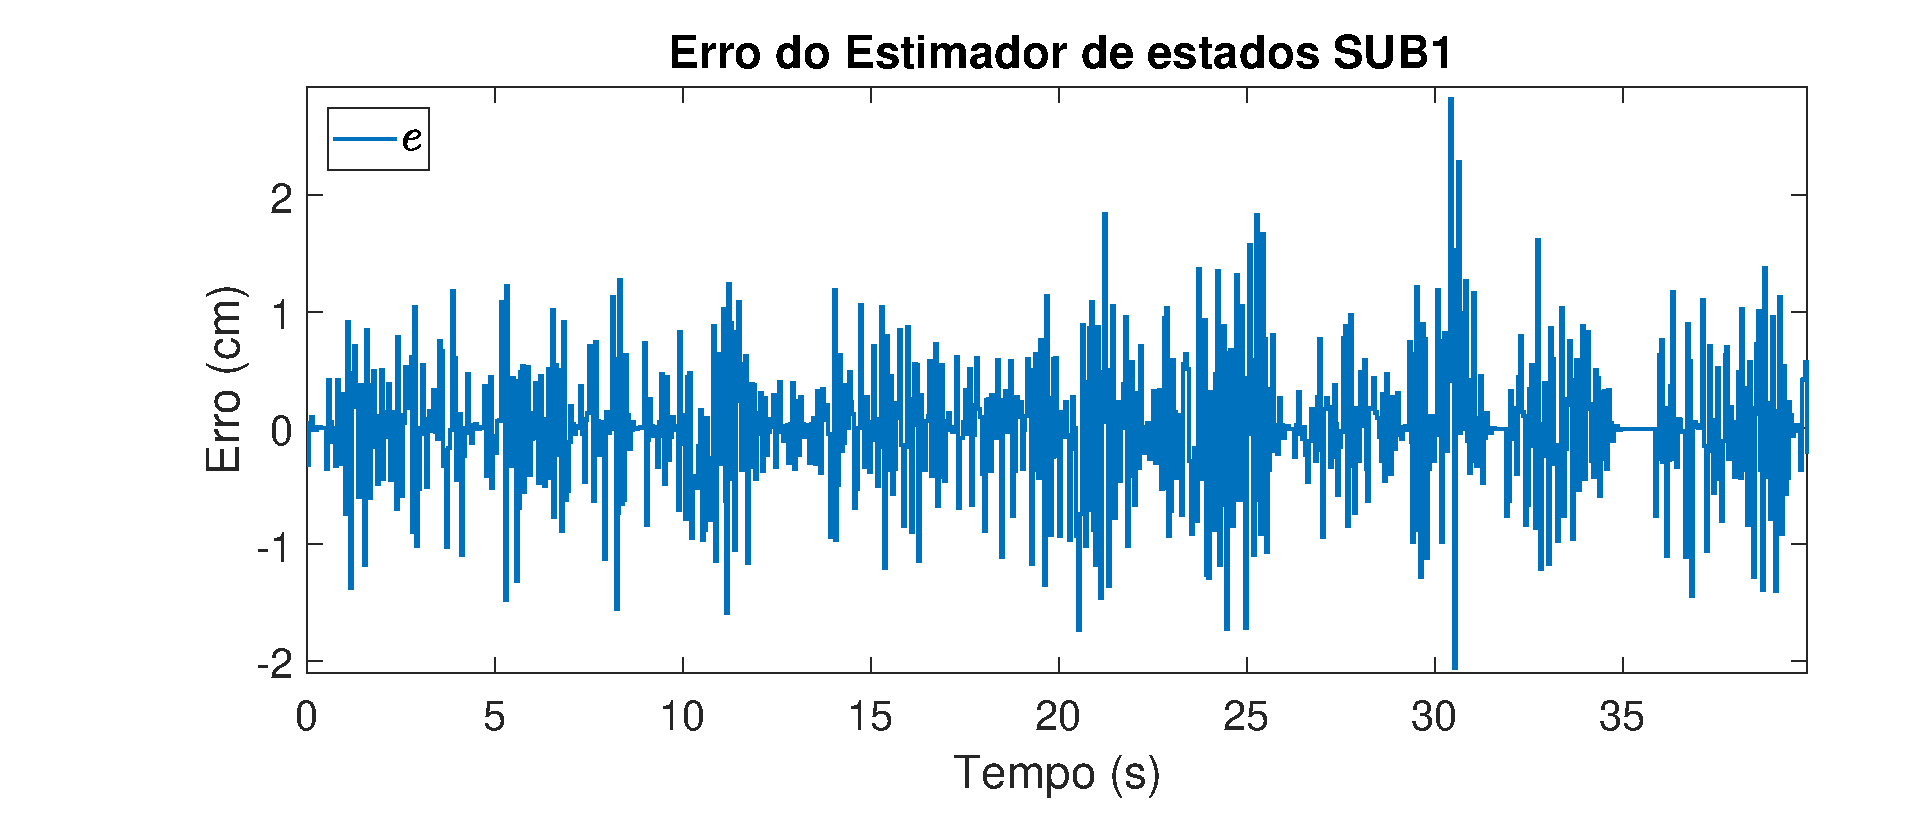
\includegraphics[width=1\linewidth]{errosub1}
	\caption[Erro do estimador do modelo $SUB1$ na resposta à escadaria]{Erro do estimador do modelo $SUB1$ na resposta à escadaria}
	\label{fig:errosub1}
\end{figure}

\begin{figure}[htb]
	\centering
	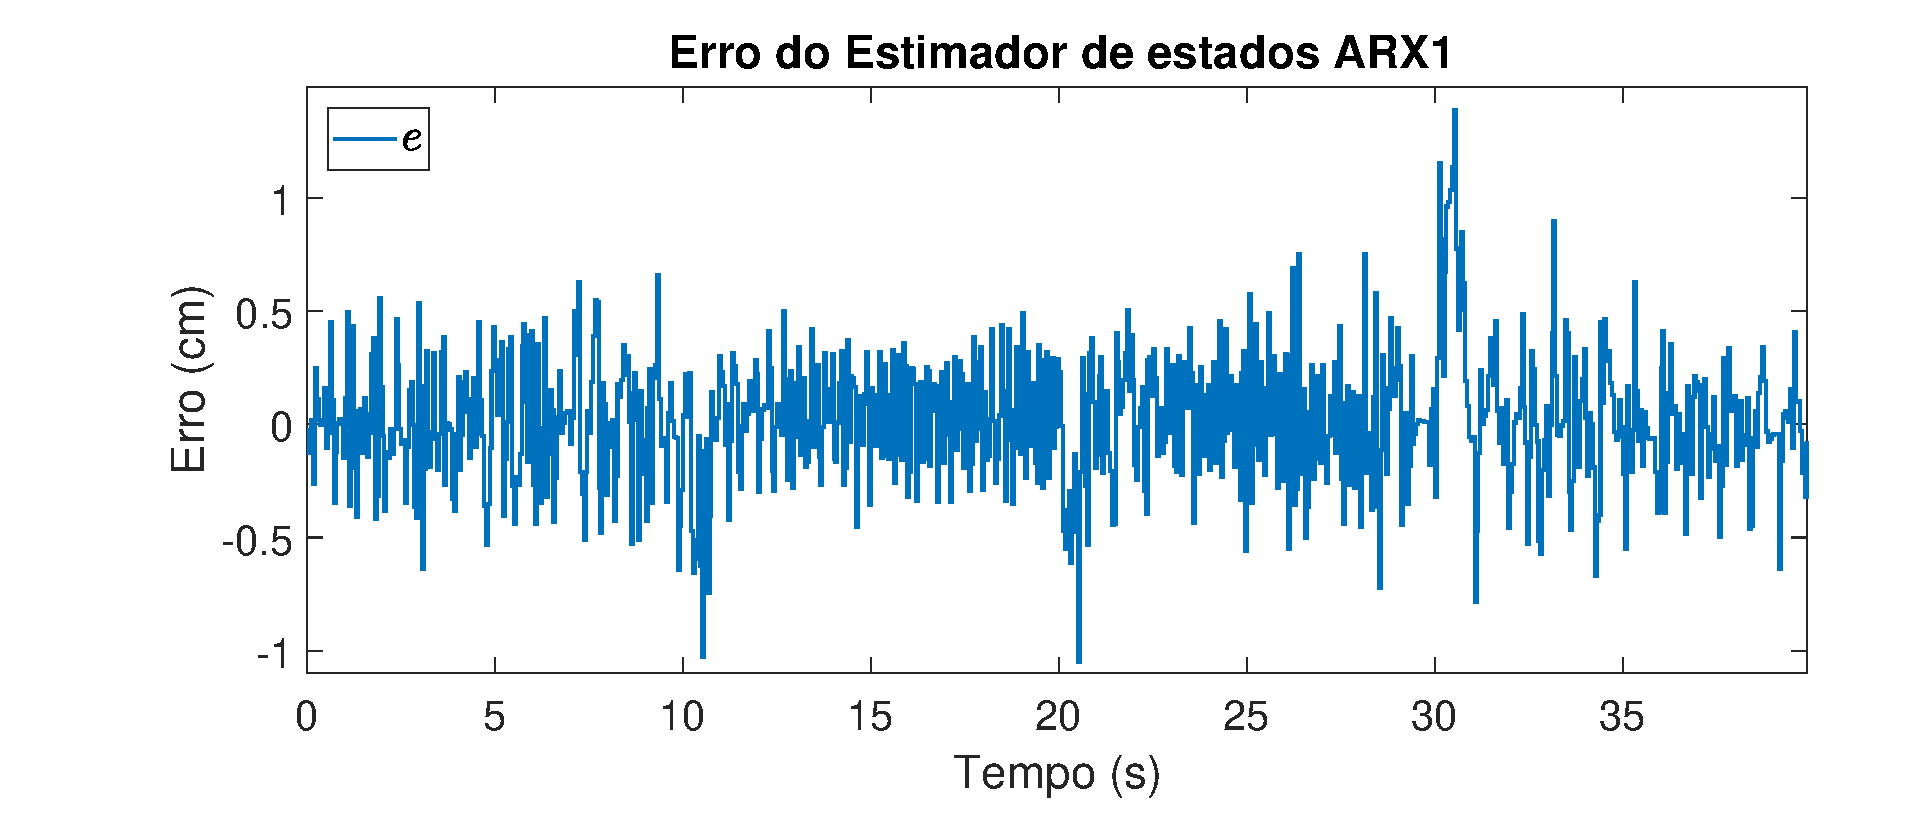
\includegraphics[width=1\linewidth]{erroarx1}
	\caption[Erro do estimador do modelo $ARX1$ na resposta à escadaria]{Erro do estimador do modelo $ARX1$ na resposta à escadaria}
	\label{fig:erroarx1}
\end{figure}

\begin{figure}[htb]
	\centering
	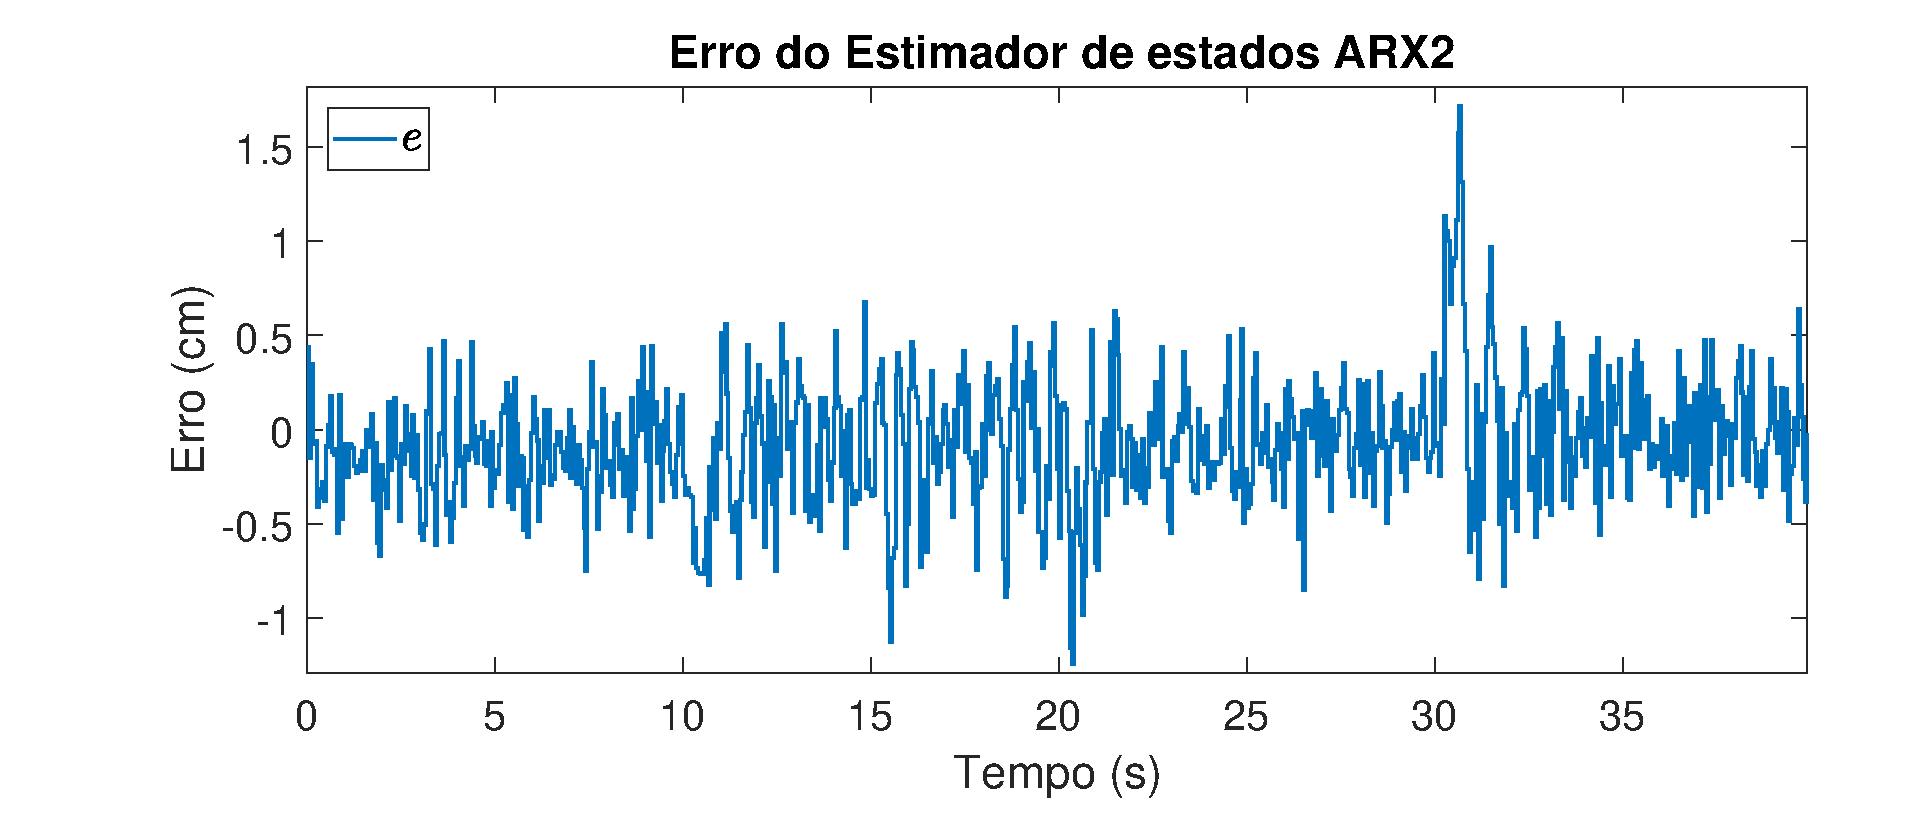
\includegraphics[width=1\linewidth]{erroarx2}
	\caption[Erro do estimador do modelo $ARX2$ na resposta à escadaria]{Erro do estimador do modelo $ARX2$ na resposta à escadaria}
	\label{fig:erroarx2}
\end{figure}


\subsection{Resultados do Teste de Robustez à mudança de Parâmetros}\label{rmp}

\subsubsection{Modelo $SUB1$}
Testamos a robustez do modelo $SUB1$ à mudança de parâmetros com o sistema real e obtemos os seguintes gráficos:
\begin{figure}[htb]
	\centering
	\begin{subfigure}[t]{0.48\textwidth}
		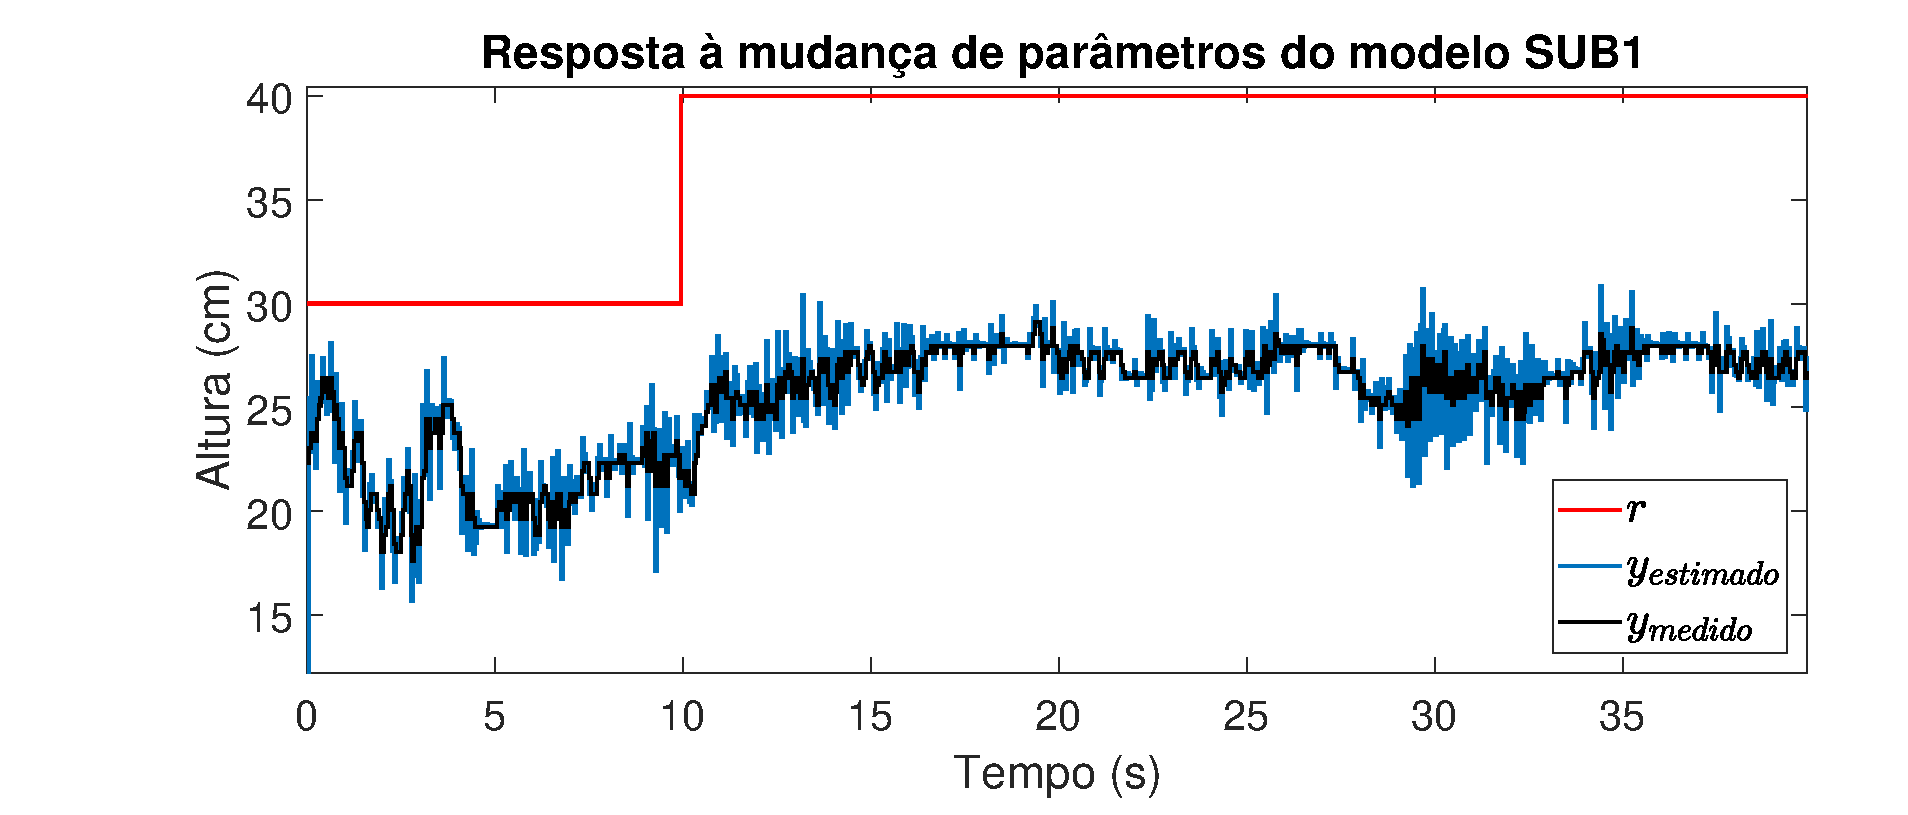
\includegraphics[width=1\linewidth]{mprsub1y}
		\caption[$y_{estimado}$ e $y_{medido}$ do modelo $SUB1$]{$y_{estimado}$ e $y_{medido}$ do modelo $SUB1$}
		\label{fig:mprsub1y}
	\end{subfigure}
	~ %add desired spacing between images, e. g. ~, \quad, \qquad, \hfill etc. 
	%(or a blank line to force the subfigure onto a new line)
	\begin{subfigure}[t]{0.48\textwidth}
		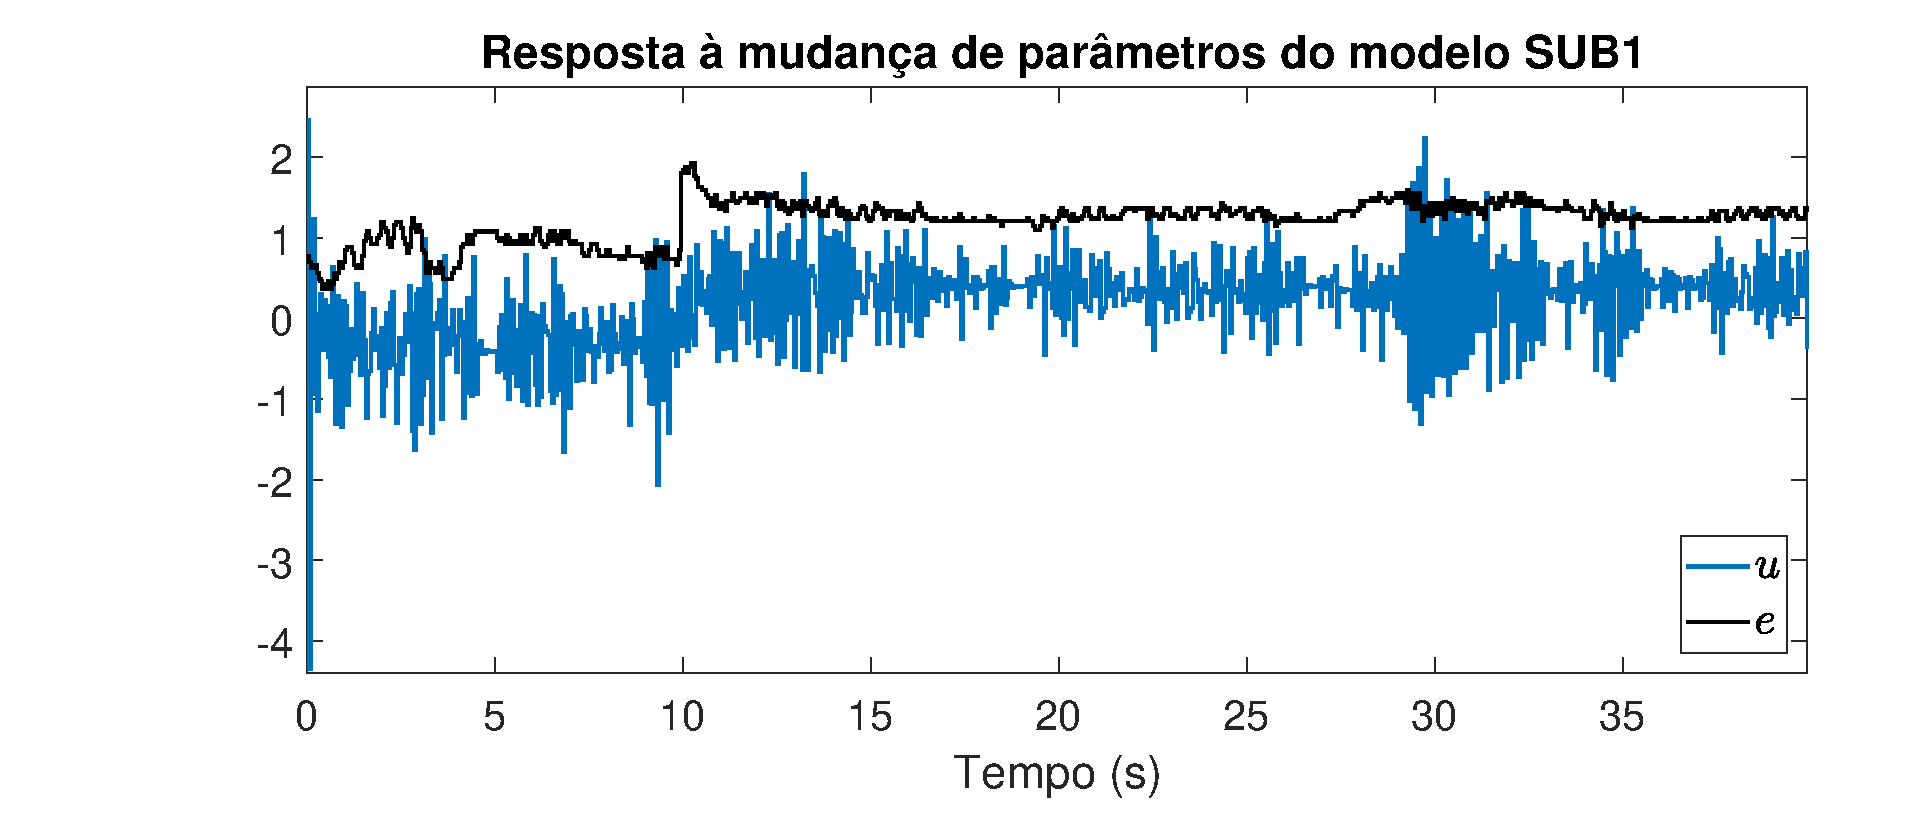
\includegraphics[width=1\linewidth]{mprsub1e}
		\caption[erro $e$ e sinal de controle $u$ do controlador $SUB1$]{erro $e$ e sinal de controle $u$ do controlador $SUB1$}
		\label{fig:mprsub1e}
	\end{subfigure}
	~ %add desired spacing between images, e. g. ~, \quad, \qquad, \hfill etc. 
	%(or a blank line to force the subfigure onto a new line)
	
	\caption{Resposta à perturbação externa do sistema com o controlador do modelo $SUB1$}\label{fig:mprsub1}
\end{figure}

Vemos na figuras \ref{fig:mprsub1y}

\subsubsection{Modelo $ARX1$}
Testamos a robustez do modelo $ARX1$ à mudança de parâmetros com o sistema real e obtemos os seguintes gráficos:
\begin{figure}[htb]
	\centering
	\begin{subfigure}[t]{0.48\textwidth}
		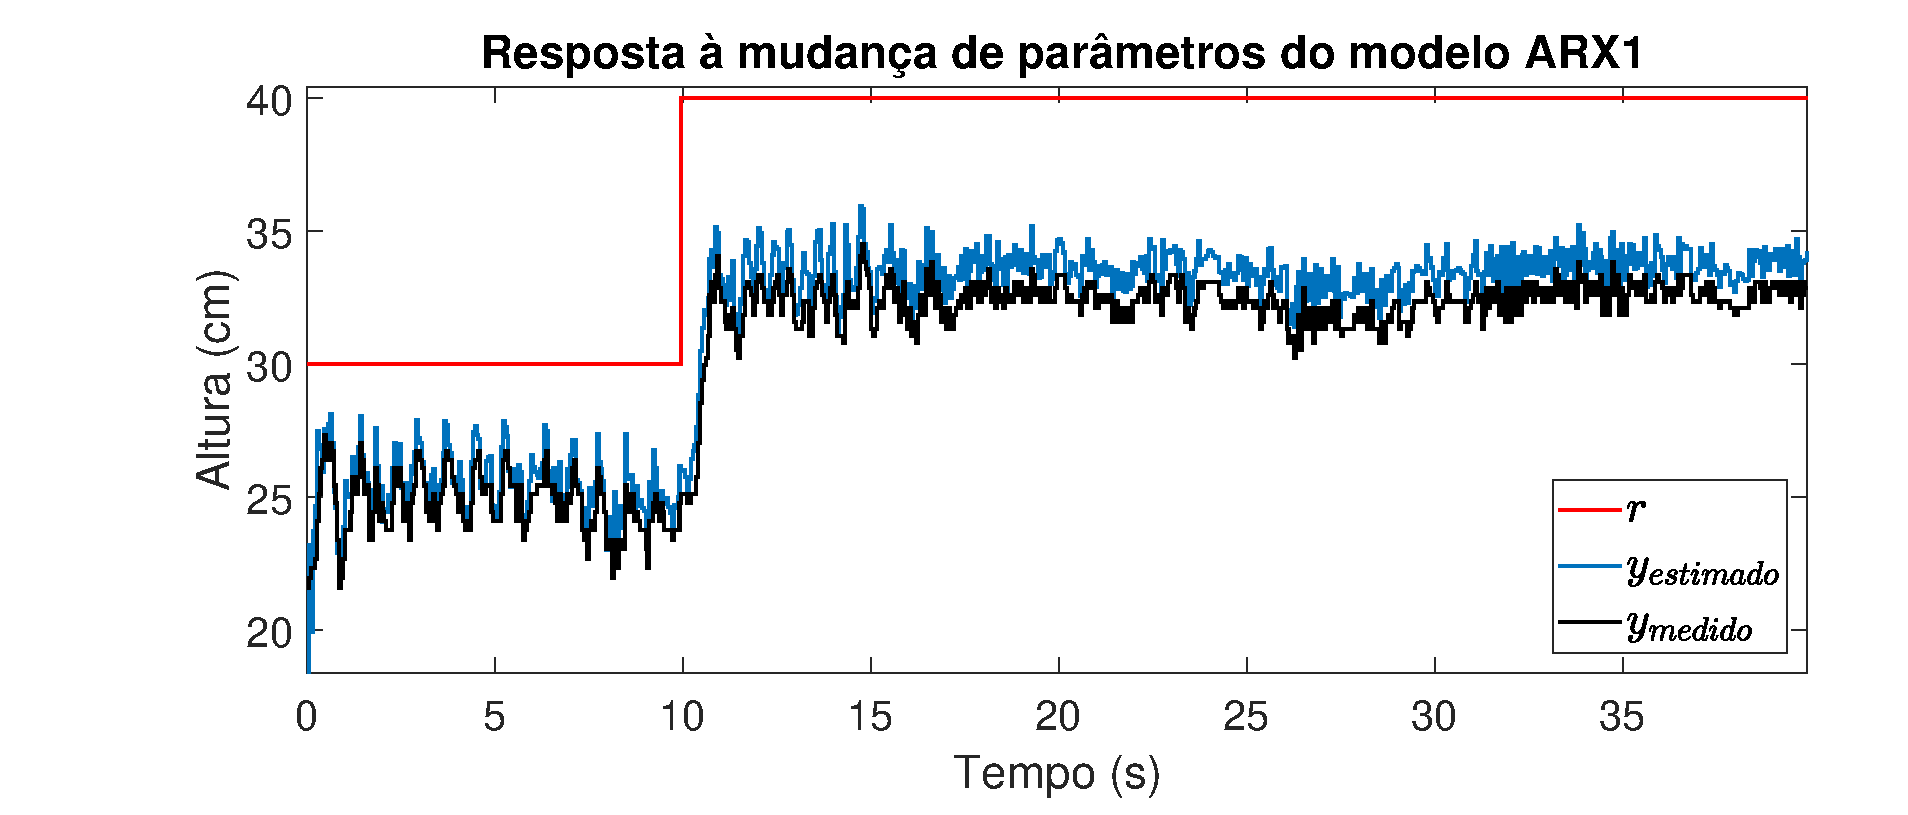
\includegraphics[width=1\linewidth]{mprarx1y}
		\caption[$y_{estimado}$ e $y_{medido}$ do modelo $ARX1$]{$y_{estimado}$ e $y_{medido}$ do modelo $ARX1$}
		\label{fig:mprarx1y}
	\end{subfigure}
	~ %add desired spacing between images, e. g. ~, \quad, \qquad, \hfill etc. 
	%(or a blank line to force the subfigure onto a new line)
	\begin{subfigure}[t]{0.48\textwidth}
		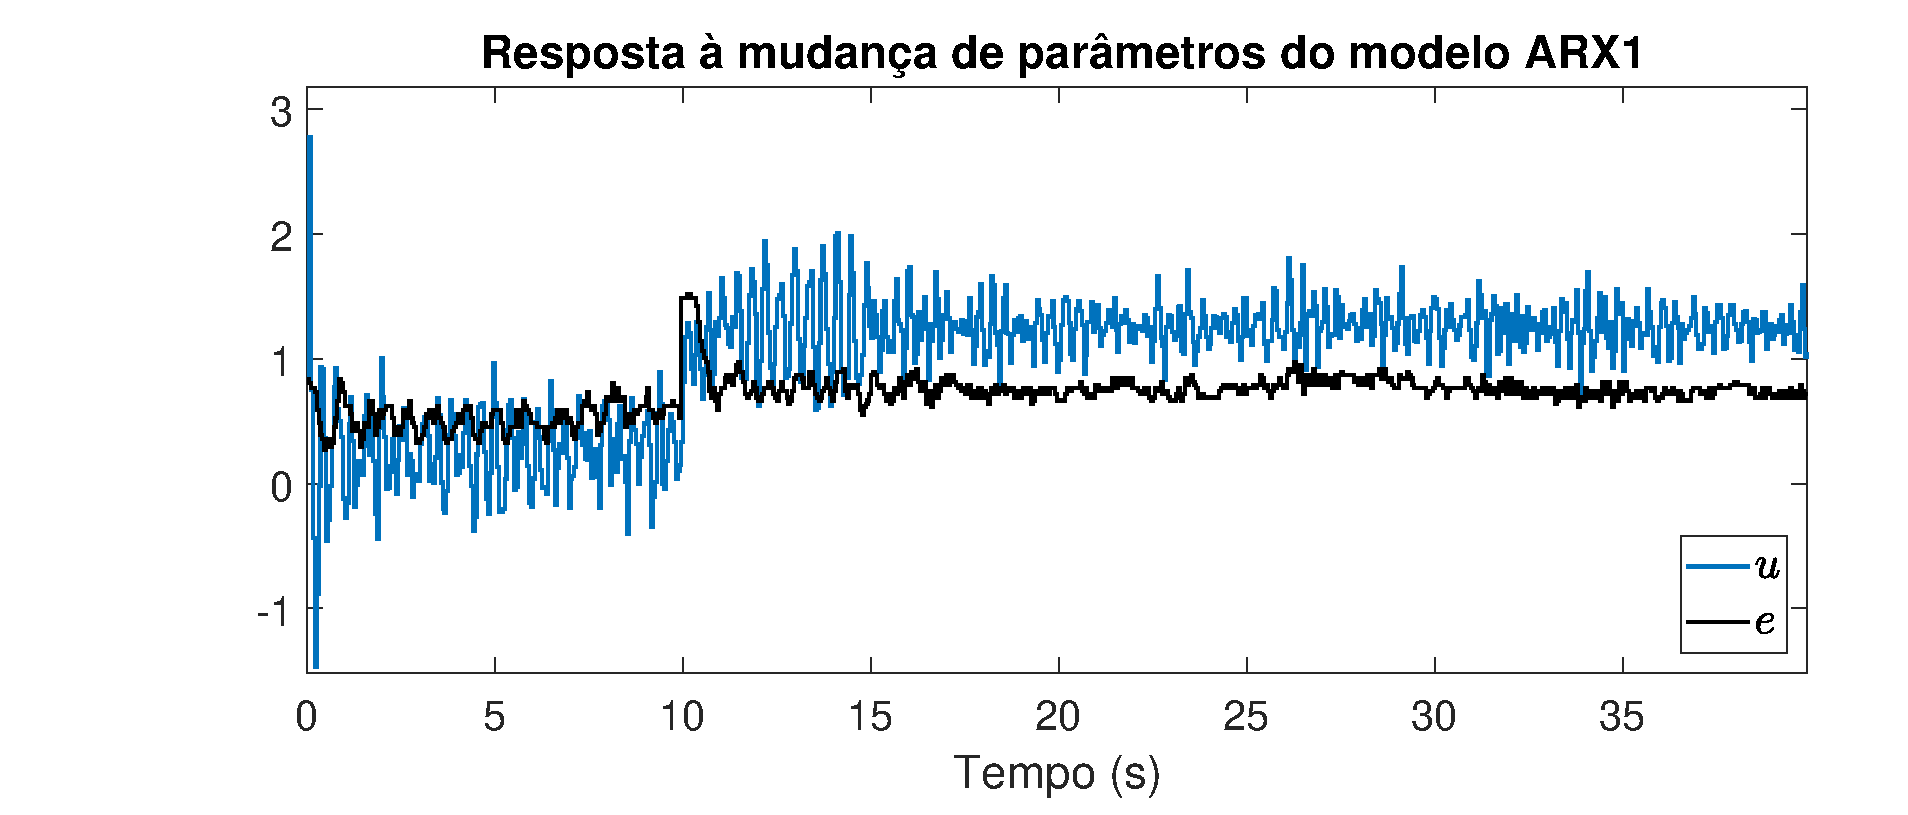
\includegraphics[width=1\linewidth]{mprarx1e}
		\caption[erro $e$ e sinal de controle $u$ do controlador $ARX1$]{erro $e$ e sinal de controle $u$ do controlador $ARX1$}
		\label{fig:mprarx1e}
	\end{subfigure}
	~ %add desired spacing between images, e. g. ~, \quad, \qquad, \hfill etc. 
	%(or a blank line to force the subfigure onto a new line)
	
	\caption{Resposta à perturbação externa do sistema com o controlador do modelo $ARX1$}\label{fig:mprarx1}
\end{figure}
Vemos na figuras \ref{fig:mprarx1y}

\subsubsection{Modelo $ARX2$}
Testamos a robustez do modelo $ARX2$ à mudança de parâmetros com o sistema real e obtemos os seguintes gráficos:
\begin{figure}[htb]
	\centering
	\begin{subfigure}[t]{0.48\textwidth}
		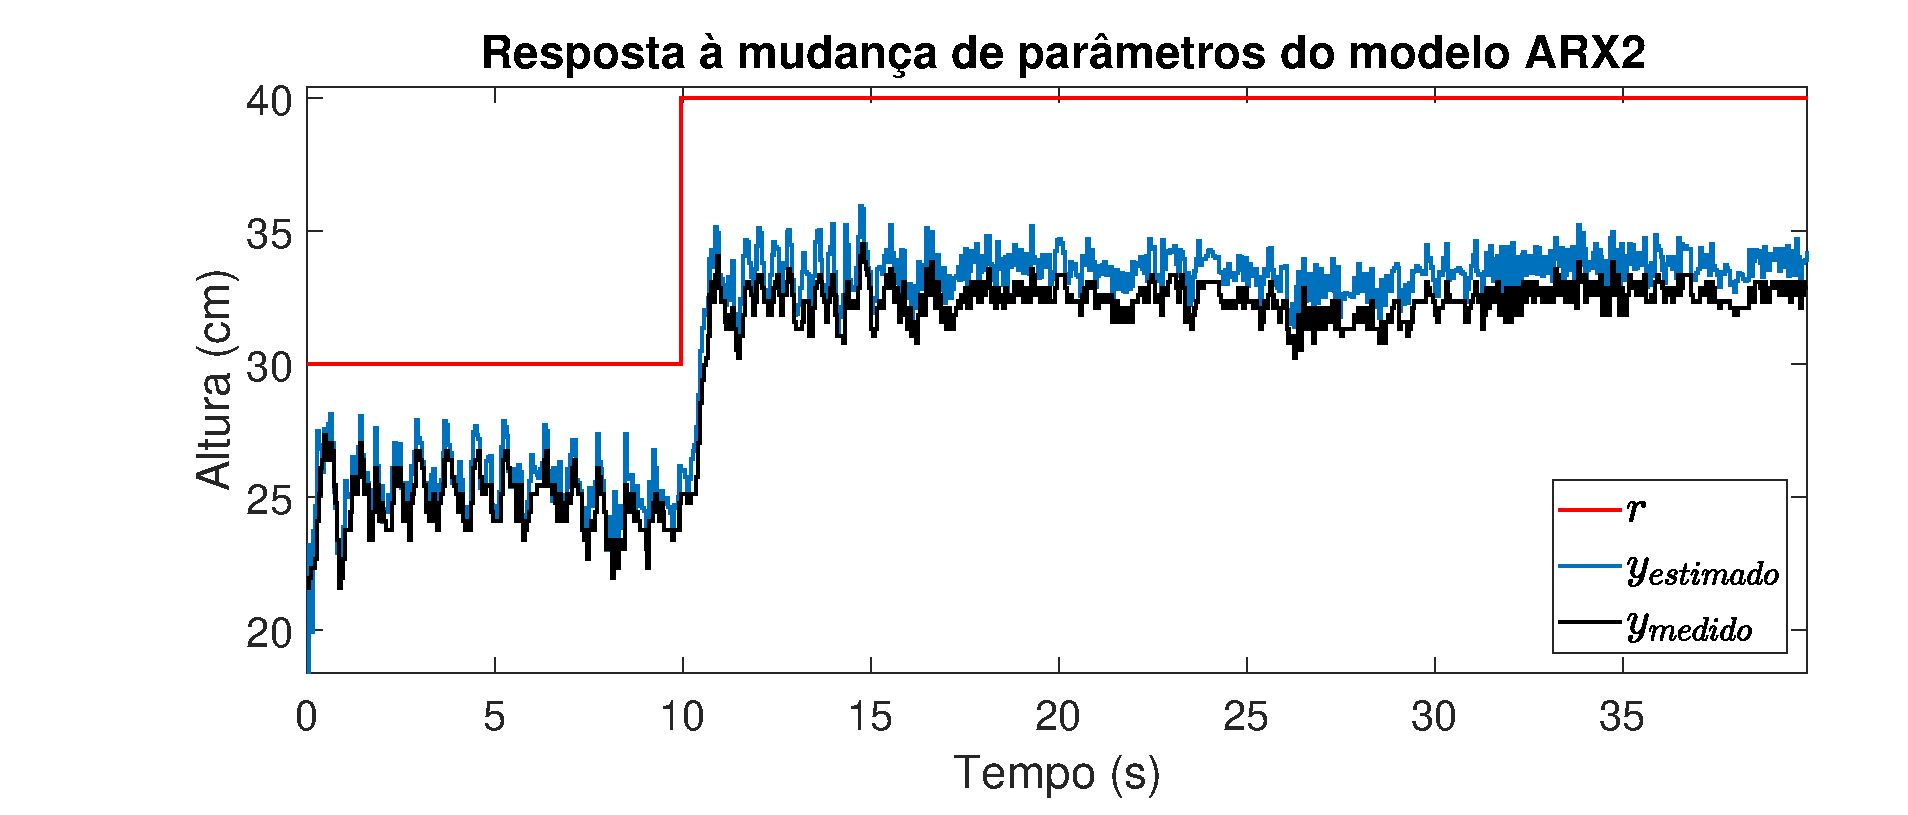
\includegraphics[width=1\linewidth]{mprarx2y}
		\caption[$y_{estimado}$ e $y_{medido}$ do modelo $ARX2$]{$y_{estimado}$ e $y_{medido}$ do modelo $ARX2$}
		\label{fig:mprarx2y}
	\end{subfigure}
	~ %add desired spacing between images, e. g. ~, \quad, \qquad, \hfill etc. 
	%(or a blank line to force the subfigure onto a new line)
	\begin{subfigure}[t]{0.48\textwidth}
		\includegraphics[width=1\linewidth]{mprarx2e}
		\caption[erro $e$ e sinal de controle $u$ do controlador $ARX2$]{erro $e$ e sinal de controle $u$ do controlador $ARX2$}
		\label{fig:mprarx2e}
	\end{subfigure}
	~ %add desired spacing between images, e. g. ~, \quad, \qquad, \hfill etc. 
	%(or a blank line to force the subfigure onto a new line)
	
	\caption{Resposta à perturbação externa do sistema com o controlador do modelo $ARX2$}\label{fig:mprarx2}
\end{figure}

Vemos na figuras \ref{fig:mprarx2y}

\subsection{Resultados do Teste de Robustez à perturbação externa}\label{rpe}

\subsubsection{Modelo $SUB1$}
Testamos a robustez do modelo $SUB1$ à perturbação externa com o sistema real e o modelo simulado e obtemos os seguintes gráficos:

\begin{figure}[htb]
	\centering
	\begin{subfigure}[t]{0.48\textwidth}
		\includegraphics[width=1\linewidth]{pextrsub1y}
		\caption[$y_{estimado}$ e $y_{medido}$ do modelo $SUB1$]{$y_{estimado}$ e $y_{medido}$ do modelo $SUB1$}
		\label{fig:pextrsub1y}
	\end{subfigure}
	~ %add desired spacing between images, e. g. ~, \quad, \qquad, \hfill etc. 
	%(or a blank line to force the subfigure onto a new line)
	\begin{subfigure}[t]{0.48\textwidth}
		\includegraphics[width=1\linewidth]{pextrsub1e}
		\caption[erro $e$ e sinal de controle $u$ do controlador $SUB1$]{erro $e$ e sinal de controle $u$ do controlador $SUB1$}
		\label{fig:pextrsub1e}
	\end{subfigure}
	~ %add desired spacing between images, e. g. ~, \quad, \qquad, \hfill etc. 
	%(or a blank line to force the subfigure onto a new line)
	
	\caption{Resposta à perturbação externa do sistema com o controlador do modelo $SUB1$}\label{fig:pextrsub1}
\end{figure}

Vemos na figuras \ref{fig:pextrsub1y}

\subsubsection{Modelo $ARX1$}
Testamos a robustez do modelo $ARX1$ à perturbação externa com o sistema real e o modelo simulado e obtemos os seguintes gráficos:
\begin{figure}[htb]
	\centering
	\begin{subfigure}[t]{0.48\textwidth}
		\includegraphics[width=1\linewidth]{pextrarx1y}
		\caption[$y_{estimado}$ e $y_{medido}$ do modelo $ARX1$]{$y_{estimado}$ e $y_{medido}$ do modelo $ARX1$}
		\label{fig:pextrarx1y}
	\end{subfigure}
	~ %add desired spacing between images, e. g. ~, \quad, \qquad, \hfill etc. 
	%(or a blank line to force the subfigure onto a new line)
	\begin{subfigure}[t]{0.48\textwidth}
		\includegraphics[width=1\linewidth]{pextrarx1e}
		\caption[erro $e$ e sinal de controle $u$ do controlador $SUB1$]{erro $e$ e sinal de controle $u$ do controlador $SUB1$}
		\label{fig:pextrarx1e}
	\end{subfigure}
	~ %add desired spacing between images, e. g. ~, \quad, \qquad, \hfill etc. 
	%(or a blank line to force the subfigure onto a new line)
	
	\caption{Resposta à perturbação externa do sistema com o controlador do modelo $ARX1$}\label{fig:pextrarx1}
\end{figure}

Vemos na figuras \ref{fig:pextrarx1y}

\subsubsection{Modelo $ARX2$}
Testamos a robustez do modelo $ARX2$ à perturbação externa com o sistema real e o modelo simulado e obtemos os seguintes gráficos:
\begin{figure}[htb]
	\centering
	\begin{subfigure}[t]{0.48\textwidth}
		\includegraphics[width=1\linewidth]{pextrarx2y}
		\caption[$y_{estimado}$ e $y_{medido}$ do modelo $ARX2$]{$y_{estimado}$ e $y_{medido}$ do modelo $ARX2$}
		\label{fig:pextrarx2y}
	\end{subfigure}
	~ %add desired spacing between images, e. g. ~, \quad, \qquad, \hfill etc. 
	%(or a blank line to force the subfigure onto a new line)
	\begin{subfigure}[t]{0.48\textwidth}
		\includegraphics[width=1\linewidth]{pextrarx2e}
		\caption[erro $e$ e sinal de controle $u$ do controlador $SUB1$]{erro $e$ e sinal de controle $u$ do controlador $SUB1$}
		\label{fig:pextrarx2e}
	\end{subfigure}
	~ %add desired spacing between images, e. g. ~, \quad, \qquad, \hfill etc. 
	%(or a blank line to force the subfigure onto a new line)
	
	\caption{Resposta à perturbação externa do sistema com o controlador do modelo $ARX2$}\label{fig:pextrarx2}
\end{figure}

Vemos na figuras \ref{fig:pextrarx2y}


\section{Discussão}

Ao analisar as respostas obtidas dos experimentos devemos levar em conta o quão ruidoso é o sensor. Apesar de aplicar um filtro na saída ele ainda produz valores que apresentam um alto valor de ruído que em conjunto com o giro da bola devido a força do vento fazem com que a leitura do sensor tenha erros que influenciam nos resultados.


Nas figuras \ref{fig:steprsub1y}, \ref{fig:steprarx1y} e \ref{fig:steprarx2y} vemos em preto a saída controlada do sistema, as linhas tracejadas em preto determinam as linhas de $\pm5\%$ da referência. Com isso medimos o tempo de assentamento para eles, 8 segundos, 6 segundos, e 6 segundos, respectivamente. Nos três casos muito além do projetado na seção \ref{s:ctrl}. Isso acontece porque passamos de um modelo idealizado do sistema para o sistema real. Apesar de termos obtido um modelo adequado para representar o sistema na simulação, o controlador gerado para ele não atende as especificações quando aplicado no sistema real. É interessante notar aqui que o estimador do modelo $SUB1$ apresenta um erro maior que o estimador dos modelos $ARX1$ e $ARX2$, isso acontece porque o método dos mínimos quadrados é um método que minimiza o resíduo, e vemos isso ser passado adiante para o estimador.


Nas figuras \ref{fig:steprsub1e}, \ref{fig:steprarx1e} e \ref{fig:steprarx2e}, vemos que o sinal de controle está trabalhando para manter o erro o menor possível, apesar de não manter erro zero.


Com a seção \ref{rstair} vemos que os controladores projetados são capazes de seguir a referência dada e trabalham para reduzir o erro. Mas nas seções \ref{rmp} e \ref{rpe} fica claro que nenhum dos controladores projetados tem capacidade para reagir à mudança de parâmetros e rejeitar perturbações externas. 


Na seção \ref{s4:val} mostramos que os 3 modelos, $SUB1$, $ARX1$ e $ARX2$, identificados à partir do sistema real são adequados para representar o sistema. O modelo $ARXsim$ identificado a partir do simulador, que continha dados experimentais do sistema sobre a velocidade do vento para diferentes PWM aplicados no motor, não apresentava as características do sistema, o que fica aparente comparando as figuras \ref{fig:sinalprbsid} e \ref{fig:sinalprbsidsimul} que mostram as diferenças entre a resposta ao sinal PRBS entre os dois. O modelo $ARXsim$ também apresenta uma resposta ao degrau, figura \ref{fig:respostadegrauarxsim}, discrepante da observada no sistema real e da observada nos outros modelos obtidos.


Essa diferença nos mostra a necessidade da identificação de um sistema usando métodos caixa-preta. Apesar de termos conseguido modelar o sistema de forma matematicamente sólida, o desempenho do modelo obtido é divergente do sistema real. Enquanto que os modelos obtidos utilizando métodos de identificação caixa-preta conseguiram gerar modelos do sistema satisfatórios. 


Na seção \ref{s:ctrl} projetamos um controlador por realimentação de estados para cada um dos modelos obtidos capaz de atender as especificações de tempo de assentamento e máximo sobrevalor definidas. Mas, devido a necessidade de criar um observador de estados na seção \ref{s5:est}, vimos que a forma como o sistema modelado atende aos requisitos mudou, mesmo se mantendo dentro dos requisitos definidos. No entanto, ao aplicar esse controlador no sistema, vemos que a resposta não está atendendo aos requisitos estabelecidos. Projetamos ainda um controlador para o modelo obtido do simulador, identificado por caixa-cinza, e ao aplicarmos no sistema real a resposta foi instável, reforçando a necessidade de obter modelos por identificação caixa-preta.


Vemos que os estimadores dos dois modelos ARX ao serem aplicados no sistema tem um bom desempenho, figuras \ref{fig:erroarx1} e \ref{fig:erroarx2}, permanecendo abaixo de 1 cm de diferença com algumas exceções, que atribuímos ao ruído do sensor. O estimador do modelo $SUB1$ não apresenta bom desempenho mostrando erros superiores a 1cm com frequência.









\chapter{Conclusão} \label{cap7}

\section{Considerações Finais}
Durante a execução deste trabalho foi construída uma plataforma de experimentos de túnel de vento vertical, atuada por uma turbina de avião RC onde a altura de uma bola é controlado pela força do vento. Foram aplicados métodos de identificação caixa preta para extrair 3 modelos diferentes do sistema e um método de identificação caixa cinza.

\section{Trabalhos Futuros}
Refazer o código de atuação do motor no sistema


% Fim Capítulo


% FOI RENOMEADO O ARQUIVO: main_tcc.bbl para main_tcc.bbl_OLD
%\bibliographystyle{IEEEtranN} % Ordem de citação
\bibliographystyle{humannat} % Ordem alfabética
%\bibliographystyle{dinat}    % Ordem alfabética
%\bibliographystyle{plainnat} % Ordem alfabética
%\bibliographystyle{apa}      % Ordem alfabética

\bibliography{referencias}

\appendix

%\chapter{TITULO APÊNDICE} \label{apendice:a}




\end{document}
